\documentclass[10pt,conference]{IEEEtran}
% Preamble of the report, loaded directly after \documentclass[10pt,conference]{IEEEtran}.
% The preamble also loads common/numbers.tex, which holds the data-set and baseline numbers as macros.
% The preamble deliberately omits hyperref, so the PDF carries no link annotations.

\usepackage[T1]{fontenc}
\usepackage{amsmath}
\usepackage{amssymb}
\usepackage{graphicx}
\usepackage{booktabs}
\usepackage{array}
\usepackage{multirow}
\usepackage{subcaption}
\usepackage{cite}              % sorted, compressed numerical citations

% Pseudocode: numbered lines, "Input:" and "Output:" headers, "for each ... do".
\usepackage{algorithm}
\usepackage{algpseudocode}
\algrenewcommand\algorithmicrequire{\textbf{Input:}}
\algrenewcommand\algorithmicensure{\textbf{Output:}}
\algrenewcommand\algorithmicforall{\textbf{for each}}

% Numbers generated by code/common/make_report_numbers.py.
% Generated by code/common/make_report_numbers.py. Do not edit by hand.
\newcommand{\nFile}{257,673}
\newcommand{\nDev}{206,139}
\newcommand{\nGen}{51,534}
\newcommand{\nNumeric}{39}
\newcommand{\nNominal}{three}
\newcommand{\nServiceMissing}{141,321}
\newcommand{\pServiceMissing}{54.8}
\newcommand{\pServiceByProtoMin}{25.7}
\newcommand{\pServiceByStateMin}{46.2}
\newcommand{\nProto}{133}
\newcommand{\nServiceCard}{13}
\newcommand{\nStateCard}{11}
\newcommand{\nProtoRare}{118}
\newcommand{\nProtoRareRows}{12,211}
\newcommand{\pProtoRareRows}{5.9}
\newcommand{\nProtoGrouped}{16}
\newcommand{\pProtoTop}{89.8}
\newcommand{\protoThreshold}{150}
\newcommand{\nFtpOut}{20}
\newcommand{\pFtpAgree}{99.997}
\newcommand{\nDup}{80,371}
\newcommand{\pDup}{39.0}
\newcommand{\nConflictVec}{2,275}
\newcommand{\nConflictRows}{32,100}
\newcommand{\pConflictRows}{15.6}
\newcommand{\pCeiling}{91.6}
\newcommand{\pFoldDup}{44.0}
\newcommand{\nCorr}{18}
\newcommand{\nLogged}{25}
\newcommand{\skewMin}{1.64}
\newcommand{\skewMax}{78.8}
\newcommand{\skewAfter}{5.38}
\newcommand{\scaleMin}{0.0043}
\newcommand{\scaleMax}{745,371}
\newcommand{\nOutlierFeatures}{16}
\newcommand{\pOutlierMax}{22.3}
\newcommand{\nClassMax}{93,000}
\newcommand{\nClassMin}{174}
\newcommand{\ratioImbalance}{534}
\newcommand{\pMajorityAccuracy}{36.1}
\newcommand{\majorityMacroF}{0.053}
\newcommand{\nWormsDev}{139}
\newcommand{\nWormsFold}{28}
\newcommand{\masterSeed}{1072417991}
\newcommand{\cpuModel}{AMD Ryzen AI 9 HX 370}
\newcommand{\logicalCores}{24}
\newcommand{\ramGB}{27}
\newcommand{\numbaThreads}{20}
\newcommand{\numbaVersion}{0.68.0}
\newcommand{\numpyVersion}{2.5.3}
\newcommand{\scipyVersion}{1.18.1}
\newcommand{\maxBins}{65,535}
\newcommand{\BlKnnAccuracyMean}{0.799}
\newcommand{\BlKnnAccuracyStd}{0.001}
\newcommand{\BlKnnAccuracyG}{0.802}
\newcommand{\BlKnnMacroFMean}{0.523}
\newcommand{\BlKnnMacroFStd}{0.010}
\newcommand{\BlKnnMacroFG}{0.516}
\newcommand{\BlKnnWeightedFMean}{0.797}
\newcommand{\BlKnnWeightedFStd}{0.001}
\newcommand{\BlKnnWeightedFG}{0.800}
\newcommand{\BlKnnBalAccMean}{0.506}
\newcommand{\BlKnnBalAccStd}{0.009}
\newcommand{\BlKnnBalAccG}{0.502}
\newcommand{\BlKnnPrepMean}{0.1}
\newcommand{\BlKnnPrepG}{0.2}
\newcommand{\BlKnnFitMean}{0.0}
\newcommand{\BlKnnFitG}{0.0}
\newcommand{\BlKnnPredictMean}{12.8}
\newcommand{\BlKnnPredictG}{20.7}
\newcommand{\BlKnnCwAccuracyMean}{0.800}
\newcommand{\BlKnnCwAccuracyStd}{0.002}
\newcommand{\BlKnnCwAccuracyG}{0.803}
\newcommand{\BlKnnCwMacroFMean}{0.528}
\newcommand{\BlKnnCwMacroFStd}{0.005}
\newcommand{\BlKnnCwMacroFG}{0.529}
\newcommand{\BlKnnCwWeightedFMean}{0.801}
\newcommand{\BlKnnCwWeightedFStd}{0.002}
\newcommand{\BlKnnCwWeightedFG}{0.804}
\newcommand{\BlKnnCwBalAccMean}{0.533}
\newcommand{\BlKnnCwBalAccStd}{0.008}
\newcommand{\BlKnnCwBalAccG}{0.530}
\newcommand{\BlKnnCwPrepMean}{0.1}
\newcommand{\BlKnnCwPrepG}{0.2}
\newcommand{\BlKnnCwFitMean}{0.0}
\newcommand{\BlKnnCwFitG}{0.0}
\newcommand{\BlKnnCwPredictMean}{13.6}
\newcommand{\BlKnnCwPredictG}{22.1}
\newcommand{\BlTreeAccuracyMean}{0.812}
\newcommand{\BlTreeAccuracyStd}{0.002}
\newcommand{\BlTreeAccuracyG}{0.816}
\newcommand{\BlTreeMacroFMean}{0.580}
\newcommand{\BlTreeMacroFStd}{0.010}
\newcommand{\BlTreeMacroFG}{0.572}
\newcommand{\BlTreeWeightedFMean}{0.806}
\newcommand{\BlTreeWeightedFStd}{0.002}
\newcommand{\BlTreeWeightedFG}{0.810}
\newcommand{\BlTreeBalAccMean}{0.566}
\newcommand{\BlTreeBalAccStd}{0.012}
\newcommand{\BlTreeBalAccG}{0.552}
\newcommand{\BlTreePrepMean}{0.1}
\newcommand{\BlTreePrepG}{0.1}
\newcommand{\BlTreeFitMean}{2.4}
\newcommand{\BlTreeFitG}{3.7}
\newcommand{\BlTreePredictMean}{0.0}
\newcommand{\BlTreePredictG}{0.0}
\newcommand{\BlTreeBalancedAccuracyMean}{0.744}
\newcommand{\BlTreeBalancedAccuracyStd}{0.007}
\newcommand{\BlTreeBalancedAccuracyG}{0.747}
\newcommand{\BlTreeBalancedMacroFMean}{0.569}
\newcommand{\BlTreeBalancedMacroFStd}{0.006}
\newcommand{\BlTreeBalancedMacroFG}{0.570}
\newcommand{\BlTreeBalancedWeightedFMean}{0.777}
\newcommand{\BlTreeBalancedWeightedFStd}{0.004}
\newcommand{\BlTreeBalancedWeightedFG}{0.777}
\newcommand{\BlTreeBalancedBalAccMean}{0.666}
\newcommand{\BlTreeBalancedBalAccStd}{0.013}
\newcommand{\BlTreeBalancedBalAccG}{0.666}
\newcommand{\BlTreeBalancedPrepMean}{0.1}
\newcommand{\BlTreeBalancedPrepG}{0.1}
\newcommand{\BlTreeBalancedFitMean}{1.9}
\newcommand{\BlTreeBalancedFitG}{2.8}
\newcommand{\BlTreeBalancedPredictMean}{0.0}
\newcommand{\BlTreeBalancedPredictG}{0.0}
\newcommand{\BlKnnK}{five}
\newcommand{\BlKnnMetric}{Manhattan}
\newcommand{\BlKnnWeights}{distance}
\newcommand{\BlKnnPower}{0}
\newcommand{\BlKnnTune}{0.520}
\newcommand{\BlKnnCwK}{15}
\newcommand{\BlKnnCwMetric}{Manhattan}
\newcommand{\BlKnnCwWeights}{distance}
\newcommand{\BlKnnCwPower}{0.25}
\newcommand{\BlKnnCwTune}{0.530}
\newcommand{\BlTreeCriterion}{entropy}
\newcommand{\BlTreeDepth}{25}
\newcommand{\BlTreeLeaf}{one}
\newcommand{\BlTreeClass}{none}
\newcommand{\BlTreeTune}{0.580}
\newcommand{\BlTreeBalancedCriterion}{entropy}
\newcommand{\BlTreeBalancedDepth}{15}
\newcommand{\BlTreeBalancedLeaf}{five}
\newcommand{\BlTreeBalancedClass}{balanced}
\newcommand{\BlTreeBalancedTune}{0.575}
\newcommand{\BlKnnFNormal}{0.916}
\newcommand{\BlKnnRNormal}{0.930}
\newcommand{\BlKnnPNormal}{0.902}
\newcommand{\BlKnnFRecon}{0.715}
\newcommand{\BlKnnRRecon}{0.733}
\newcommand{\BlKnnPRecon}{0.698}
\newcommand{\BlKnnFBackdoor}{0.096}
\newcommand{\BlKnnRBackdoor}{0.077}
\newcommand{\BlKnnPBackdoor}{0.128}
\newcommand{\BlKnnFDoS}{0.393}
\newcommand{\BlKnnRDoS}{0.450}
\newcommand{\BlKnnPDoS}{0.349}
\newcommand{\BlKnnFExploits}{0.680}
\newcommand{\BlKnnRExploits}{0.684}
\newcommand{\BlKnnPExploits}{0.676}
\newcommand{\BlKnnFAnalysis}{0.170}
\newcommand{\BlKnnRAnalysis}{0.107}
\newcommand{\BlKnnPAnalysis}{0.422}
\newcommand{\BlKnnFFuzzers}{0.610}
\newcommand{\BlKnnRFuzzers}{0.554}
\newcommand{\BlKnnPFuzzers}{0.679}
\newcommand{\BlKnnFWorms}{0.130}
\newcommand{\BlKnnRWorms}{0.086}
\newcommand{\BlKnnPWorms}{0.273}
\newcommand{\BlKnnFShellcode}{0.462}
\newcommand{\BlKnnRShellcode}{0.417}
\newcommand{\BlKnnPShellcode}{0.516}
\newcommand{\BlKnnFGeneric}{0.987}
\newcommand{\BlKnnRGeneric}{0.977}
\newcommand{\BlKnnPGeneric}{0.996}
\newcommand{\BlKnnDoSAsExploits}{1,452}
\newcommand{\BlKnnExploitsAsDoS}{1,858}
\newcommand{\BlKnnNormalAsFuzzers}{980}
\newcommand{\BlKnnFuzzersAsNormal}{1,431}
\newcommand{\BlKnnWormsHit}{three}
\newcommand{\BlKnnWormsSupport}{35}
\newcommand{\BlKnnCwFNormal}{0.917}
\newcommand{\BlKnnCwRNormal}{0.913}
\newcommand{\BlKnnCwPNormal}{0.922}
\newcommand{\BlKnnCwFRecon}{0.738}
\newcommand{\BlKnnCwRRecon}{0.759}
\newcommand{\BlKnnCwPRecon}{0.717}
\newcommand{\BlKnnCwFBackdoor}{0.058}
\newcommand{\BlKnnCwRBackdoor}{0.049}
\newcommand{\BlKnnCwPBackdoor}{0.070}
\newcommand{\BlKnnCwFDoS}{0.381}
\newcommand{\BlKnnCwRDoS}{0.427}
\newcommand{\BlKnnCwPDoS}{0.343}
\newcommand{\BlKnnCwFExploits}{0.690}
\newcommand{\BlKnnCwRExploits}{0.692}
\newcommand{\BlKnnCwPExploits}{0.687}
\newcommand{\BlKnnCwFAnalysis}{0.155}
\newcommand{\BlKnnCwRAnalysis}{0.110}
\newcommand{\BlKnnCwPAnalysis}{0.262}
\newcommand{\BlKnnCwFFuzzers}{0.628}
\newcommand{\BlKnnCwRFuzzers}{0.616}
\newcommand{\BlKnnCwPFuzzers}{0.641}
\newcommand{\BlKnnCwFWorms}{0.254}
\newcommand{\BlKnnCwRWorms}{0.229}
\newcommand{\BlKnnCwPWorms}{0.286}
\newcommand{\BlKnnCwFShellcode}{0.483}
\newcommand{\BlKnnCwRShellcode}{0.533}
\newcommand{\BlKnnCwPShellcode}{0.442}
\newcommand{\BlKnnCwFGeneric}{0.987}
\newcommand{\BlKnnCwRGeneric}{0.976}
\newcommand{\BlKnnCwPGeneric}{0.998}
\newcommand{\BlKnnCwDoSAsExploits}{1,608}
\newcommand{\BlKnnCwExploitsAsDoS}{1,799}
\newcommand{\BlKnnCwNormalAsFuzzers}{1,249}
\newcommand{\BlKnnCwFuzzersAsNormal}{1,090}
\newcommand{\BlKnnCwWormsHit}{eight}
\newcommand{\BlKnnCwWormsSupport}{35}
\newcommand{\BlTreeFNormal}{0.924}
\newcommand{\BlTreeRNormal}{0.939}
\newcommand{\BlTreePNormal}{0.910}
\newcommand{\BlTreeFRecon}{0.823}
\newcommand{\BlTreeRRecon}{0.760}
\newcommand{\BlTreePRecon}{0.896}
\newcommand{\BlTreeFBackdoor}{0.180}
\newcommand{\BlTreeRBackdoor}{0.109}
\newcommand{\BlTreePBackdoor}{0.505}
\newcommand{\BlTreeFDoS}{0.321}
\newcommand{\BlTreeRDoS}{0.306}
\newcommand{\BlTreePDoS}{0.336}
\newcommand{\BlTreeFExploits}{0.699}
\newcommand{\BlTreeRExploits}{0.772}
\newcommand{\BlTreePExploits}{0.639}
\newcommand{\BlTreeFAnalysis}{0.162}
\newcommand{\BlTreeRAnalysis}{0.095}
\newcommand{\BlTreePAnalysis}{0.543}
\newcommand{\BlTreeFFuzzers}{0.617}
\newcommand{\BlTreeRFuzzers}{0.565}
\newcommand{\BlTreePFuzzers}{0.679}
\newcommand{\BlTreeFWorms}{0.417}
\newcommand{\BlTreeRWorms}{0.429}
\newcommand{\BlTreePWorms}{0.405}
\newcommand{\BlTreeFShellcode}{0.591}
\newcommand{\BlTreeRShellcode}{0.556}
\newcommand{\BlTreePShellcode}{0.629}
\newcommand{\BlTreeFGeneric}{0.987}
\newcommand{\BlTreeRGeneric}{0.984}
\newcommand{\BlTreePGeneric}{0.989}
\newcommand{\BlTreeDoSAsExploits}{2,120}
\newcommand{\BlTreeExploitsAsDoS}{1,367}
\newcommand{\BlTreeNormalAsFuzzers}{924}
\newcommand{\BlTreeFuzzersAsNormal}{1,450}
\newcommand{\BlTreeWormsHit}{15}
\newcommand{\BlTreeWormsSupport}{35}
\newcommand{\BlTreeBalancedFNormal}{0.846}
\newcommand{\BlTreeBalancedRNormal}{0.740}
\newcommand{\BlTreeBalancedPNormal}{0.987}
\newcommand{\BlTreeBalancedFRecon}{0.819}
\newcommand{\BlTreeBalancedRRecon}{0.820}
\newcommand{\BlTreeBalancedPRecon}{0.818}
\newcommand{\BlTreeBalancedFBackdoor}{0.103}
\newcommand{\BlTreeBalancedRBackdoor}{0.315}
\newcommand{\BlTreeBalancedPBackdoor}{0.062}
\newcommand{\BlTreeBalancedFDoS}{0.438}
\newcommand{\BlTreeBalancedRDoS}{0.571}
\newcommand{\BlTreeBalancedPDoS}{0.355}
\newcommand{\BlTreeBalancedFExploits}{0.637}
\newcommand{\BlTreeBalancedRExploits}{0.504}
\newcommand{\BlTreeBalancedPExploits}{0.865}
\newcommand{\BlTreeBalancedFAnalysis}{0.115}
\newcommand{\BlTreeBalancedRAnalysis}{0.224}
\newcommand{\BlTreeBalancedPAnalysis}{0.078}
\newcommand{\BlTreeBalancedFFuzzers}{0.612}
\newcommand{\BlTreeBalancedRFuzzers}{0.820}
\newcommand{\BlTreeBalancedPFuzzers}{0.488}
\newcommand{\BlTreeBalancedFWorms}{0.577}
\newcommand{\BlTreeBalancedRWorms}{0.800}
\newcommand{\BlTreeBalancedPWorms}{0.452}
\newcommand{\BlTreeBalancedFShellcode}{0.568}
\newcommand{\BlTreeBalancedRShellcode}{0.887}
\newcommand{\BlTreeBalancedPShellcode}{0.418}
\newcommand{\BlTreeBalancedFGeneric}{0.988}
\newcommand{\BlTreeBalancedRGeneric}{0.980}
\newcommand{\BlTreeBalancedPGeneric}{0.997}
\newcommand{\BlTreeBalancedDoSAsExploits}{308}
\newcommand{\BlTreeBalancedExploitsAsDoS}{2,310}
\newcommand{\BlTreeBalancedNormalAsFuzzers}{3,986}
\newcommand{\BlTreeBalancedFuzzersAsNormal}{140}
\newcommand{\BlTreeBalancedWormsHit}{28}
\newcommand{\BlTreeBalancedWormsSupport}{35}
\newcommand{\StTreeKnnAccuracyDiff}{0.012}
\newcommand{\StTreeKnnAccuracyAbsDiff}{0.012}
\newcommand{\StTreeKnnAccuracyDz}{6.6}
\newcommand{\StTreeKnnAccuracyWil}{$p < 0.001$}
\newcommand{\StTreeKnnAccuracyCor}{$p < 0.001$}
\newcommand{\StTreeKnnMacroFDiff}{0.057}
\newcommand{\StTreeKnnMacroFAbsDiff}{0.057}
\newcommand{\StTreeKnnMacroFDz}{4.9}
\newcommand{\StTreeKnnMacroFWil}{$p < 0.001$}
\newcommand{\StTreeKnnMacroFCor}{$p < 0.001$}
\newcommand{\StTreeKnnWeightedFDiff}{0.009}
\newcommand{\StTreeKnnWeightedFAbsDiff}{0.009}
\newcommand{\StTreeKnnWeightedFDz}{5.0}
\newcommand{\StTreeKnnWeightedFWil}{$p < 0.001$}
\newcommand{\StTreeKnnWeightedFCor}{$p < 0.001$}
\newcommand{\StTreeKnnBalAccDiff}{0.060}
\newcommand{\StTreeKnnBalAccAbsDiff}{0.060}
\newcommand{\StTreeKnnBalAccDz}{4.6}
\newcommand{\StTreeKnnBalAccWil}{$p < 0.001$}
\newcommand{\StTreeKnnBalAccCor}{$p < 0.001$}
\newcommand{\StTreeKnnCwAccuracyDiff}{0.011}
\newcommand{\StTreeKnnCwAccuracyAbsDiff}{0.011}
\newcommand{\StTreeKnnCwAccuracyDz}{6.7}
\newcommand{\StTreeKnnCwAccuracyWil}{$p < 0.001$}
\newcommand{\StTreeKnnCwAccuracyCor}{$p < 0.001$}
\newcommand{\StTreeKnnCwMacroFDiff}{0.052}
\newcommand{\StTreeKnnCwMacroFAbsDiff}{0.052}
\newcommand{\StTreeKnnCwMacroFDz}{5.7}
\newcommand{\StTreeKnnCwMacroFWil}{$p < 0.001$}
\newcommand{\StTreeKnnCwMacroFCor}{$p < 0.001$}
\newcommand{\StTreeKnnCwWeightedFDiff}{0.005}
\newcommand{\StTreeKnnCwWeightedFAbsDiff}{0.005}
\newcommand{\StTreeKnnCwWeightedFDz}{3.0}
\newcommand{\StTreeKnnCwWeightedFWil}{$p < 0.001$}
\newcommand{\StTreeKnnCwWeightedFCor}{$p < 0.001$}
\newcommand{\StTreeKnnCwBalAccDiff}{0.033}
\newcommand{\StTreeKnnCwBalAccAbsDiff}{0.033}
\newcommand{\StTreeKnnCwBalAccDz}{2.8}
\newcommand{\StTreeKnnCwBalAccWil}{$p < 0.001$}
\newcommand{\StTreeKnnCwBalAccCor}{$p < 0.001$}
\newcommand{\StKnnCwKnnAccuracyDiff}{0.001}
\newcommand{\StKnnCwKnnAccuracyAbsDiff}{0.001}
\newcommand{\StKnnCwKnnAccuracyDz}{0.6}
\newcommand{\StKnnCwKnnAccuracyWil}{$p = 0.030$}
\newcommand{\StKnnCwKnnAccuracyCor}{$p = 0.276$}
\newcommand{\StKnnCwKnnMacroFDiff}{0.005}
\newcommand{\StKnnCwKnnMacroFAbsDiff}{0.005}
\newcommand{\StKnnCwKnnMacroFDz}{0.7}
\newcommand{\StKnnCwKnnMacroFWil}{$p = 0.012$}
\newcommand{\StKnnCwKnnMacroFCor}{$p = 0.253$}
\newcommand{\StKnnCwKnnWeightedFDiff}{0.004}
\newcommand{\StKnnCwKnnWeightedFAbsDiff}{0.004}
\newcommand{\StKnnCwKnnWeightedFDz}{3.3}
\newcommand{\StKnnCwKnnWeightedFWil}{$p < 0.001$}
\newcommand{\StKnnCwKnnWeightedFCor}{$p < 0.001$}
\newcommand{\StKnnCwKnnBalAccDiff}{0.027}
\newcommand{\StKnnCwKnnBalAccAbsDiff}{0.027}
\newcommand{\StKnnCwKnnBalAccDz}{5.6}
\newcommand{\StKnnCwKnnBalAccWil}{$p < 0.001$}
\newcommand{\StKnnCwKnnBalAccCor}{$p < 0.001$}
\newcommand{\StTreeBalancedKnnAccuracyDiff}{-0.055}
\newcommand{\StTreeBalancedKnnAccuracyAbsDiff}{0.055}
\newcommand{\StTreeBalancedKnnAccuracyDz}{-8.9}
\newcommand{\StTreeBalancedKnnAccuracyWil}{$p < 0.001$}
\newcommand{\StTreeBalancedKnnAccuracyCor}{$p < 0.001$}
\newcommand{\StTreeBalancedKnnMacroFDiff}{0.047}
\newcommand{\StTreeBalancedKnnMacroFAbsDiff}{0.047}
\newcommand{\StTreeBalancedKnnMacroFDz}{4.1}
\newcommand{\StTreeBalancedKnnMacroFWil}{$p < 0.001$}
\newcommand{\StTreeBalancedKnnMacroFCor}{$p < 0.001$}
\newcommand{\StTreeBalancedKnnWeightedFDiff}{-0.020}
\newcommand{\StTreeBalancedKnnWeightedFAbsDiff}{0.020}
\newcommand{\StTreeBalancedKnnWeightedFDz}{-5.2}
\newcommand{\StTreeBalancedKnnWeightedFWil}{$p < 0.001$}
\newcommand{\StTreeBalancedKnnWeightedFCor}{$p < 0.001$}
\newcommand{\StTreeBalancedKnnBalAccDiff}{0.159}
\newcommand{\StTreeBalancedKnnBalAccAbsDiff}{0.159}
\newcommand{\StTreeBalancedKnnBalAccDz}{11.9}
\newcommand{\StTreeBalancedKnnBalAccWil}{$p < 0.001$}
\newcommand{\StTreeBalancedKnnBalAccCor}{$p < 0.001$}
\newcommand{\StTreeBalancedKnnCwAccuracyDiff}{-0.056}
\newcommand{\StTreeBalancedKnnCwAccuracyAbsDiff}{0.056}
\newcommand{\StTreeBalancedKnnCwAccuracyDz}{-9.8}
\newcommand{\StTreeBalancedKnnCwAccuracyWil}{$p < 0.001$}
\newcommand{\StTreeBalancedKnnCwAccuracyCor}{$p < 0.001$}
\newcommand{\StTreeBalancedKnnCwMacroFDiff}{0.042}
\newcommand{\StTreeBalancedKnnCwMacroFAbsDiff}{0.042}
\newcommand{\StTreeBalancedKnnCwMacroFDz}{5.8}
\newcommand{\StTreeBalancedKnnCwMacroFWil}{$p < 0.001$}
\newcommand{\StTreeBalancedKnnCwMacroFCor}{$p < 0.001$}
\newcommand{\StTreeBalancedKnnCwWeightedFDiff}{-0.024}
\newcommand{\StTreeBalancedKnnCwWeightedFAbsDiff}{0.024}
\newcommand{\StTreeBalancedKnnCwWeightedFDz}{-7.2}
\newcommand{\StTreeBalancedKnnCwWeightedFWil}{$p < 0.001$}
\newcommand{\StTreeBalancedKnnCwWeightedFCor}{$p < 0.001$}
\newcommand{\StTreeBalancedKnnCwBalAccDiff}{0.133}
\newcommand{\StTreeBalancedKnnCwBalAccAbsDiff}{0.133}
\newcommand{\StTreeBalancedKnnCwBalAccDz}{11.0}
\newcommand{\StTreeBalancedKnnCwBalAccWil}{$p < 0.001$}
\newcommand{\StTreeBalancedKnnCwBalAccCor}{$p < 0.001$}
\newcommand{\StTreeBalancedTreeAccuracyDiff}{-0.067}
\newcommand{\StTreeBalancedTreeAccuracyAbsDiff}{0.067}
\newcommand{\StTreeBalancedTreeAccuracyDz}{-9.6}
\newcommand{\StTreeBalancedTreeAccuracyWil}{$p < 0.001$}
\newcommand{\StTreeBalancedTreeAccuracyCor}{$p < 0.001$}
\newcommand{\StTreeBalancedTreeMacroFDiff}{-0.011}
\newcommand{\StTreeBalancedTreeMacroFAbsDiff}{0.011}
\newcommand{\StTreeBalancedTreeMacroFDz}{-1.0}
\newcommand{\StTreeBalancedTreeMacroFWil}{$p = 0.001$}
\newcommand{\StTreeBalancedTreeMacroFCor}{$p = 0.085$}
\newcommand{\StTreeBalancedTreeWeightedFDiff}{-0.029}
\newcommand{\StTreeBalancedTreeWeightedFAbsDiff}{0.029}
\newcommand{\StTreeBalancedTreeWeightedFDz}{-6.6}
\newcommand{\StTreeBalancedTreeWeightedFWil}{$p < 0.001$}
\newcommand{\StTreeBalancedTreeWeightedFCor}{$p < 0.001$}
\newcommand{\StTreeBalancedTreeBalAccDiff}{0.100}
\newcommand{\StTreeBalancedTreeBalAccAbsDiff}{0.100}
\newcommand{\StTreeBalancedTreeBalAccDz}{6.5}
\newcommand{\StTreeBalancedTreeBalAccWil}{$p < 0.001$}
\newcommand{\StTreeBalancedTreeBalAccCor}{$p < 0.001$}
\newcommand{\weakFMax}{0.180}
\newcommand{\gMaxDiff}{0.015}
\newcommand{\nTestFold}{41,228}
\newcommand{\FriedmanCD}{1.21}
\newcommand{\rtTuneKnn}{2.4}
\newcommand{\rtTuneTree}{2.4}
\newcommand{\rtCompare}{7.7}
\newcommand{\rtFinal}{0.8}
\newcommand{\BlTreeNodes}{18,743}
\newcommand{\BlTreeLeaves}{9,372}
\newcommand{\BlTreeDepthG}{25}
\newcommand{\AbKnnFullColumns}{74}
\newcommand{\AbKnnNoRareColumns}{191}
\newcommand{\AbKnnFullMacroF}{0.520}
\newcommand{\AbKnnFullAccuracy}{0.800}
\newcommand{\AbKnnNoLogMacroF}{0.490}
\newcommand{\AbKnnNoLogAccuracy}{0.781}
\newcommand{\AbKnnNoStdMacroF}{0.387}
\newcommand{\AbKnnNoStdAccuracy}{0.669}
\newcommand{\AbKnnNoLogStdMacroF}{0.379}
\newcommand{\AbKnnNoLogStdAccuracy}{0.664}
\newcommand{\AbKnnRedundantMacroF}{0.518}
\newcommand{\AbKnnRedundantAccuracy}{0.800}
\newcommand{\AbKnnNoRareMacroF}{0.519}
\newcommand{\AbKnnNoRareAccuracy}{0.799}
\newcommand{\AbTreeRawMacroF}{0.580}
\newcommand{\AbTreeRawAccuracy}{0.811}
\newcommand{\AbTreeLogStdMacroF}{0.580}
\newcommand{\AbTreeLogStdAccuracy}{0.811}
\newcommand{\AbTreeDroppedMacroF}{0.578}
\newcommand{\AbTreeDroppedAccuracy}{0.811}
\newcommand{\AbTreeNoRareMacroF}{0.582}
\newcommand{\AbTreeNoRareAccuracy}{0.814}
\newcommand{\AbTreeBinsLowMacroF}{0.565}
\newcommand{\AbTreeBinsLowAccuracy}{0.809}
\newcommand{\AbTreeBinsMidMacroF}{0.582}
\newcommand{\AbTreeBinsMidAccuracy}{0.811}


% Bibliography: alphabetical by the surname of the first author.
\bibliographystyle{IEEEtranS}

% Notation macros (one meaning per symbol).
\newcommand{\vect}[1]{\mathbf{#1}}          % vectors: bold lower case
\newcommand{\mat}[1]{\mathbf{#1}}           % matrices: bold upper case
\DeclareMathOperator*{\argmax}{arg\,max}
\DeclareMathOperator*{\argmin}{arg\,min}

% Generated by code/ensemble/make_report_numbers.py. Do not edit by hand.
\newcommand{\OATwoKnnAccuracy}{0.802}
\newcommand{\OATwoKnnMacroF}{0.525}
\newcommand{\OATwoKnnWeightedF}{0.799}
\newcommand{\OATwoKnnBalAcc}{0.507}
\newcommand{\OATwoTreeAccuracy}{0.759}
\newcommand{\OATwoTreeMacroF}{0.576}
\newcommand{\OATwoTreeWeightedF}{0.790}
\newcommand{\OATwoTreeBalAcc}{0.609}
\newcommand{\OKnnGrid}{160}
\newcommand{\OTreeGrid}{168}
\newcommand{\OConfZero}{1}
\newcommand{\OConfOne}{16}
\newcommand{\OConfTwo}{85}
\newcommand{\OConfThree}{77}
\newcommand{\OConfFour}{37}
\newcommand{\OConfFive}{76}
\newcommand{\OConfSix}{15}
\newcommand{\OConfSeven}{6}
\newcommand{\OConfEight}{1}
\newcommand{\OConfNine}{1}
\newcommand{\OGcCleanDoSExpl}{51}
\newcommand{\OGcCleanExplDoS}{1}
\newcommand{\OGcCleanBackDoS}{5}
\newcommand{\OGcCleanAnalDoS}{3}
\newcommand{\OGcCleanDoSDoS}{39}
\newcommand{\OGcCleanRows}{84.3}
\newcommand{\OGcCleanAcc}{0.916}
\newcommand{\OGcConfDoSExpl}{18}
\newcommand{\OGcConfExplDoS}{79}
\newcommand{\OGcConfBackDoS}{65}
\newcommand{\OGcConfAnalDoS}{68}
\newcommand{\OGcConfDoSDoS}{78}
\newcommand{\OGcConfRows}{15.7}
\newcommand{\OGcConfAcc}{0.327}
\newcommand{\OPcMaxRunSd}{0.016}
\newcommand{\OEncOneF}{0.602}
\newcommand{\OEncOneFStd}{0.010}
\newcommand{\OEncOneAcc}{0.832}
\newcommand{\OEncOneBal}{0.576}
\newcommand{\OEncOrdF}{0.595}
\newcommand{\OEncOrdFStd}{0.010}
\newcommand{\OEncOrdAcc}{0.831}
\newcommand{\OEncOrdBal}{0.566}
\newcommand{\OEncDiff}{0.007}
\newcommand{\OFeatOneF}{0.528}
\newcommand{\OFeatOneFStd}{0.006}
\newcommand{\OFeatOneOob}{0.528}
\newcommand{\OFeatOneBal}{0.503}
\newcommand{\OFeatOneAcc}{0.822}
\newcommand{\OFeatOneS}{0.775}
\newcommand{\OFeatOneA}{0.197}
\newcommand{\OFeatOneQ}{0.890}
\newcommand{\OFeatOneNodes}{32,997}
\newcommand{\OFeatTwoF}{0.546}
\newcommand{\OFeatTwoFStd}{0.006}
\newcommand{\OFeatTwoOob}{0.548}
\newcommand{\OFeatTwoBal}{0.521}
\newcommand{\OFeatTwoAcc}{0.826}
\newcommand{\OFeatTwoS}{0.784}
\newcommand{\OFeatTwoA}{0.187}
\newcommand{\OFeatTwoQ}{0.896}
\newcommand{\OFeatTwoNodes}{26,448}
\newcommand{\OFeatFourF}{0.569}
\newcommand{\OFeatFourFStd}{0.015}
\newcommand{\OFeatFourOob}{0.572}
\newcommand{\OFeatFourBal}{0.542}
\newcommand{\OFeatFourAcc}{0.829}
\newcommand{\OFeatFourS}{0.791}
\newcommand{\OFeatFourA}{0.177}
\newcommand{\OFeatFourQ}{0.902}
\newcommand{\OFeatFourNodes}{22,001}
\newcommand{\OFeatEightF}{0.602}
\newcommand{\OFeatEightFStd}{0.008}
\newcommand{\OFeatEightOob}{0.601}
\newcommand{\OFeatEightBal}{0.576}
\newcommand{\OFeatEightAcc}{0.832}
\newcommand{\OFeatEightS}{0.796}
\newcommand{\OFeatEightA}{0.171}
\newcommand{\OFeatEightQ}{0.906}
\newcommand{\OFeatEightNodes}{19,210}
\newcommand{\OFeatSixteenF}{0.616}
\newcommand{\OFeatSixteenFStd}{0.002}
\newcommand{\OFeatSixteenOob}{0.613}
\newcommand{\OFeatSixteenBal}{0.595}
\newcommand{\OFeatSixteenAcc}{0.833}
\newcommand{\OFeatSixteenS}{0.798}
\newcommand{\OFeatSixteenA}{0.167}
\newcommand{\OFeatSixteenQ}{0.909}
\newcommand{\OFeatSixteenNodes}{17,621}
\newcommand{\OFeatThirtyTwoF}{0.615}
\newcommand{\OFeatThirtyTwoFStd}{0.005}
\newcommand{\OFeatThirtyTwoOob}{0.615}
\newcommand{\OFeatThirtyTwoBal}{0.595}
\newcommand{\OFeatThirtyTwoAcc}{0.833}
\newcommand{\OFeatThirtyTwoS}{0.799}
\newcommand{\OFeatThirtyTwoA}{0.166}
\newcommand{\OFeatThirtyTwoQ}{0.911}
\newcommand{\OFeatThirtyTwoNodes}{16,943}
\newcommand{\OFeatAllF}{0.609}
\newcommand{\OFeatAllFStd}{0.005}
\newcommand{\OFeatAllOob}{0.608}
\newcommand{\OFeatAllBal}{0.589}
\newcommand{\OFeatAllAcc}{0.830}
\newcommand{\OFeatAllS}{0.799}
\newcommand{\OFeatAllA}{0.163}
\newcommand{\OFeatAllQ}{0.915}
\newcommand{\OFeatAllNodes}{16,900}
\newcommand{\OFeatBest}{16}
\newcommand{\OFeatEncoded}{79}
\newcommand{\OFeatSqrt}{8}
\newcommand{\OFeatEffOne}{-0.075}
\newcommand{\OFeatEffSizeOne}{-6.6}
\newcommand{\OFeatEffTwo}{-0.057}
\newcommand{\OFeatEffSizeTwo}{-5.8}
\newcommand{\OFeatEffFour}{-0.034}
\newcommand{\OFeatEffSizeFour}{-3.7}
\newcommand{\OFeatEffSixteen}{0.013}
\newcommand{\OFeatEffSizeSixteen}{1.8}
\newcommand{\OFeatEffThirtyTwo}{0.012}
\newcommand{\OFeatEffSizeThirtyTwo}{1.3}
\newcommand{\OFeatEffAll}{0.006}
\newcommand{\OFeatEffSizeAll}{0.5}
\newcommand{\ODepthThreeLeafOneF}{0.250}
\newcommand{\ODepthFiveLeafOneF}{0.335}
\newcommand{\ODepthEightLeafOneF}{0.436}
\newcommand{\ODepthTwelveLeafOneF}{0.532}
\newcommand{\ODepthTwentyLeafOneF}{0.592}
\newcommand{\ODepthNoneLeafOneF}{0.601}
\newcommand{\ODepthNoneLeafTwoF}{0.602}
\newcommand{\ODepthNoneLeafFiftyF}{0.493}
\newcommand{\ODepthTwentyLeafFiftyF}{0.492}
\newcommand{\ODepthNoneLeafFiveF}{0.586}
\newcommand{\ODepthNoneLeafTenF}{0.554}
\newcommand{\ODepthNoneLeafTwentyFiveF}{0.513}
\newcommand{\OLeafOneRTwo}{0.093}
\newcommand{\OLeafOneRFive}{0.111}
\newcommand{\OLeafOneRSeven}{0.434}
\newcommand{\OLeafTwentyFiveRTwo}{0.049}
\newcommand{\OLeafTwentyFiveRFive}{0.037}
\newcommand{\OLeafTwentyFiveRSeven}{0.000}
\newcommand{\ODepthNoneLeafOneNodes}{19,206}
\newcommand{\ODepthNoneLeafFiftyNodes}{1,559}
\newcommand{\ODepthNoneLeafOneS}{0.796}
\newcommand{\ODepthNoneLeafTwentyFiveS}{0.804}
\newcommand{\ODepthTwelveLeafOneS}{0.806}
\newcommand{\ODepthNoneLeafOneAcc}{0.832}
\newcommand{\ODepthTwentyLeafOneAcc}{0.832}
\newcommand{\ODepthBestF}{0.602}
\newcommand{\OTrPlainF}{0.601}
\newcommand{\OTrPlainAcc}{0.832}
\newcommand{\OTrPlainBal}{0.574}
\newcommand{\OTrPlainRSeven}{0.446}
\newcommand{\OTrPlainRTwo}{0.092}
\newcommand{\OTrPlainRFive}{0.112}
\newcommand{\OTrPlainREight}{0.689}
\newcommand{\OTrPlainFSeven}{0.526}
\newcommand{\OTrPlainOob}{0.599}
\newcommand{\OTrPlainRSevenStd}{0.139}
\newcommand{\OTrPlainFStd}{0.009}
\newcommand{\OTrWeightHalfF}{0.614}
\newcommand{\OTrWeightHalfAcc}{0.825}
\newcommand{\OTrWeightHalfBal}{0.603}
\newcommand{\OTrWeightHalfRSeven}{0.546}
\newcommand{\OTrWeightHalfRTwo}{0.124}
\newcommand{\OTrWeightHalfRFive}{0.123}
\newcommand{\OTrWeightHalfREight}{0.687}
\newcommand{\OTrWeightHalfFSeven}{0.595}
\newcommand{\OTrWeightHalfOob}{0.614}
\newcommand{\OTrWeightHalfRSevenStd}{0.109}
\newcommand{\OTrWeightHalfFStd}{0.007}
\newcommand{\OTrWeightFullF}{0.592}
\newcommand{\OTrWeightFullAcc}{0.800}
\newcommand{\OTrWeightFullBal}{0.588}
\newcommand{\OTrWeightFullRSeven}{0.575}
\newcommand{\OTrWeightFullRTwo}{0.189}
\newcommand{\OTrWeightFullRFive}{0.152}
\newcommand{\OTrWeightFullREight}{0.675}
\newcommand{\OTrWeightFullFSeven}{0.619}
\newcommand{\OTrWeightFullOob}{0.590}
\newcommand{\OTrWeightFullRSevenStd}{0.091}
\newcommand{\OTrWeightFullFStd}{0.008}
\newcommand{\OTrBootHalfF}{0.631}
\newcommand{\OTrBootHalfAcc}{0.823}
\newcommand{\OTrBootHalfBal}{0.640}
\newcommand{\OTrBootHalfRSeven}{0.690}
\newcommand{\OTrBootHalfRTwo}{0.168}
\newcommand{\OTrBootHalfRFive}{0.140}
\newcommand{\OTrBootHalfREight}{0.783}
\newcommand{\OTrBootHalfFSeven}{0.682}
\newcommand{\OTrBootHalfOob}{0.541}
\newcommand{\OTrBootHalfRSevenStd}{0.052}
\newcommand{\OTrBootHalfFStd}{0.003}
\newcommand{\OTrBootHalfWeightHalfF}{0.594}
\newcommand{\OTrBootHalfWeightHalfAcc}{0.790}
\newcommand{\OTrBootHalfWeightHalfBal}{0.606}
\newcommand{\OTrBootHalfWeightHalfRSeven}{0.694}
\newcommand{\OTrBootHalfWeightHalfRTwo}{0.217}
\newcommand{\OTrBootHalfWeightHalfRFive}{0.149}
\newcommand{\OTrBootHalfWeightHalfREight}{0.773}
\newcommand{\OTrBootHalfWeightHalfFSeven}{0.678}
\newcommand{\OTrBootHalfWeightHalfOob}{0.508}
\newcommand{\OTrBootHalfWeightHalfRSevenStd}{0.052}
\newcommand{\OTrBootHalfWeightHalfFStd}{0.005}
\newcommand{\OTrBootFullF}{0.588}
\newcommand{\OTrBootFullAcc}{0.774}
\newcommand{\OTrBootFullBal}{0.617}
\newcommand{\OTrBootFullRSeven}{0.712}
\newcommand{\OTrBootFullRTwo}{0.223}
\newcommand{\OTrBootFullRFive}{0.166}
\newcommand{\OTrBootFullREight}{0.802}
\newcommand{\OTrBootFullFSeven}{0.676}
\newcommand{\OTrBootFullOob}{0.443}
\newcommand{\OTrBootFullRSevenStd}{0.058}
\newcommand{\OTrBootFullFStd}{0.005}
\newcommand{\OTrUnderMinF}{0.481}
\newcommand{\OTrUnderMinAcc}{0.709}
\newcommand{\OTrUnderMinBal}{0.661}
\newcommand{\OTrUnderMinRSeven}{0.946}
\newcommand{\OTrUnderMinRTwo}{0.326}
\newcommand{\OTrUnderMinRFive}{0.309}
\newcommand{\OTrUnderMinREight}{0.938}
\newcommand{\OTrUnderMinFSeven}{0.076}
\newcommand{\OTrUnderMinOob}{0.480}
\newcommand{\OTrUnderMinRSevenStd}{0.078}
\newcommand{\OTrUnderMinFStd}{0.003}
\newcommand{\OTrUnderThousandF}{0.531}
\newcommand{\OTrUnderThousandAcc}{0.728}
\newcommand{\OTrUnderThousandBal}{0.650}
\newcommand{\OTrUnderThousandRSeven}{0.889}
\newcommand{\OTrUnderThousandRTwo}{0.229}
\newcommand{\OTrUnderThousandRFive}{0.276}
\newcommand{\OTrUnderThousandREight}{0.963}
\newcommand{\OTrUnderThousandFSeven}{0.478}
\newcommand{\OTrUnderThousandOob}{0.485}
\newcommand{\OTrUnderThousandRSevenStd}{0.088}
\newcommand{\OTrUnderThousandFStd}{0.006}
\newcommand{\OTrEffBootHalf}{0.030}
\newcommand{\OTrEffSizeBootHalf}{3.8}
\newcommand{\OTrEffBootHalfWeightHalf}{-0.007}
\newcommand{\OTrEffSizeBootHalfWeightHalf}{-1.0}
\newcommand{\OTrEffWeightHalf}{0.014}
\newcommand{\OTrEffSizeWeightHalf}{1.8}
\newcommand{\OSizePlainOneF}{0.553}
\newcommand{\OSizePlainOneFStd}{0.010}
\newcommand{\OSizePlainTenF}{0.600}
\newcommand{\OSizePlainTenFStd}{0.012}
\newcommand{\OSizePlainFiftyF}{0.611}
\newcommand{\OSizePlainFiftyFStd}{0.008}
\newcommand{\OSizePlainHundredF}{0.614}
\newcommand{\OSizePlainHundredFStd}{0.004}
\newcommand{\OSizePlainTwoHundredF}{0.616}
\newcommand{\OSizePlainTwoHundredFStd}{0.004}
\newcommand{\OSizePlainFiveHundredF}{0.616}
\newcommand{\OSizePlainFiveHundredFStd}{0.004}
\newcommand{\OSizePlainTwoThousandF}{0.616}
\newcommand{\OSizePlainTwoThousandFStd}{0.003}
\newcommand{\OSizePlainDimAt}{50}
\newcommand{\OSizePlainOobDimAt}{100}
\newcommand{\OSizePlainOob}{0.615}
\newcommand{\OSizePlainDis}{0.169}
\newcommand{\OSizePlainStrength}{0.797}
\newcommand{\OSizePlainAcc}{0.833}
\newcommand{\OSizePlainOneAcc}{0.797}
\newcommand{\OSizePlainGainLast}{+0.0006}
\newcommand{\OSizePlainCoverageTwo}{0.600}
\newcommand{\OSizeWeightedOneF}{0.577}
\newcommand{\OSizeWeightedOneFStd}{0.011}
\newcommand{\OSizeWeightedTenF}{0.623}
\newcommand{\OSizeWeightedTenFStd}{0.005}
\newcommand{\OSizeWeightedFiftyF}{0.633}
\newcommand{\OSizeWeightedFiftyFStd}{0.003}
\newcommand{\OSizeWeightedHundredF}{0.634}
\newcommand{\OSizeWeightedHundredFStd}{0.003}
\newcommand{\OSizeWeightedTwoHundredF}{0.634}
\newcommand{\OSizeWeightedTwoHundredFStd}{0.003}
\newcommand{\OSizeWeightedFiveHundredF}{0.634}
\newcommand{\OSizeWeightedFiveHundredFStd}{0.003}
\newcommand{\OSizeWeightedTwoThousandF}{0.635}
\newcommand{\OSizeWeightedTwoThousandFStd}{0.003}
\newcommand{\OSizeWeightedDimAt}{20}
\newcommand{\OSizeWeightedOobDimAt}{70}
\newcommand{\OSizeWeightedOob}{0.634}
\newcommand{\OSizeWeightedDis}{0.163}
\newcommand{\OSizeWeightedStrength}{0.788}
\newcommand{\OSizeWeightedAcc}{0.823}
\newcommand{\OSizeWeightedOneAcc}{0.788}
\newcommand{\OSizeWeightedGainLast}{+0.0003}
\newcommand{\OSizeWeightedCoverageTwo}{0.600}
\newcommand{\OSizeSampledOneF}{0.573}
\newcommand{\OSizeSampledOneFStd}{0.009}
\newcommand{\OSizeSampledTenF}{0.620}
\newcommand{\OSizeSampledTenFStd}{0.008}
\newcommand{\OSizeSampledFiftyF}{0.631}
\newcommand{\OSizeSampledFiftyFStd}{0.005}
\newcommand{\OSizeSampledHundredF}{0.633}
\newcommand{\OSizeSampledHundredFStd}{0.005}
\newcommand{\OSizeSampledTwoHundredF}{0.634}
\newcommand{\OSizeSampledTwoHundredFStd}{0.005}
\newcommand{\OSizeSampledFiveHundredF}{0.634}
\newcommand{\OSizeSampledFiveHundredFStd}{0.005}
\newcommand{\OSizeSampledTwoThousandF}{0.634}
\newcommand{\OSizeSampledTwoThousandFStd}{0.006}
\newcommand{\OSizeSampledDimAt}{50}
\newcommand{\OSizeSampledOobDimAt}{1000}
\newcommand{\OSizeSampledOob}{0.559}
\newcommand{\OSizeSampledDis}{0.172}
\newcommand{\OSizeSampledStrength}{0.786}
\newcommand{\OSizeSampledAcc}{0.824}
\newcommand{\OSizeSampledOneAcc}{0.787}
\newcommand{\OSizeSampledGainLast}{+0.0002}
\newcommand{\OSizeSampledCoverageTwo}{0.637}
\newcommand{\OBoostPeakAt}{200}
\newcommand{\OBoostLast}{1000}
\newcommand{\OBoostPeakF}{0.618}
\newcommand{\OBoostPeakFStd}{0.009}
\newcommand{\OBoostPeakTrain}{0.090}
\newcommand{\OBoostPeakDis}{0.249}
\newcommand{\OBoostPeakAcc}{0.820}
\newcommand{\OBoostLastF}{0.597}
\newcommand{\OBoostLastFStd}{0.009}
\newcommand{\OBoostLastTrain}{0.090}
\newcommand{\OBoostLastDis}{0.338}
\newcommand{\OBoostLastAcc}{0.817}
\newcommand{\OBoostOneF}{0.597}
\newcommand{\OBoostOneFStd}{0.005}
\newcommand{\OBoostOneTrain}{0.126}
\newcommand{\OBoostOneDis}{0.000}
\newcommand{\OBoostOneAcc}{0.802}
\newcommand{\OJStageOne}{160}
\newcommand{\OJStageTwo}{23}
\newcommand{\OJPlainF}{0.616}
\newcommand{\OJPlainFStd}{0.005}
\newcommand{\OJPlainConfig}{j031}
\newcommand{\OJPlainFeatures}{24}
\newcommand{\OJPlainDepth}{none}
\newcommand{\OJPlainLeaf}{2}
\newcommand{\OJPlainCriterion}{entropy}
\newcommand{\OJPlainAlpha}{0.0}
\newcommand{\OJPlainOmega}{0.0}
\newcommand{\OJPlainSampler}{bootstrap}
\newcommand{\OJPlainSize}{none}
\newcommand{\OJPlainAcc}{0.833}
\newcommand{\OJPlainBal}{0.597}
\newcommand{\OJWeightedF}{0.634}
\newcommand{\OJWeightedFStd}{0.003}
\newcommand{\OJWeightedConfig}{j043}
\newcommand{\OJWeightedFeatures}{16}
\newcommand{\OJWeightedDepth}{20}
\newcommand{\OJWeightedLeaf}{3}
\newcommand{\OJWeightedCriterion}{entropy}
\newcommand{\OJWeightedAlpha}{0.5}
\newcommand{\OJWeightedOmega}{0.0}
\newcommand{\OJWeightedSampler}{bootstrap}
\newcommand{\OJWeightedSize}{none}
\newcommand{\OJWeightedAcc}{0.823}
\newcommand{\OJWeightedBal}{0.654}
\newcommand{\OJSampledF}{0.634}
\newcommand{\OJSampledFStd}{0.005}
\newcommand{\OJSampledConfig}{f4}
\newcommand{\OJSampledFeatures}{16}
\newcommand{\OJSampledDepth}{none}
\newcommand{\OJSampledLeaf}{1}
\newcommand{\OJSampledCriterion}{entropy}
\newcommand{\OJSampledAlpha}{0.0}
\newcommand{\OJSampledOmega}{0.5}
\newcommand{\OJSampledSampler}{bootstrap}
\newcommand{\OJSampledSize}{none}
\newcommand{\OJSampledAcc}{0.824}
\newcommand{\OJSampledBal}{0.647}
\newcommand{\OJBothF}{0.634}
\newcommand{\OJBothFStd}{0.007}
\newcommand{\OJBothConfig}{j121}
\newcommand{\OJBothFeatures}{24}
\newcommand{\OJBothDepth}{20}
\newcommand{\OJBothLeaf}{1}
\newcommand{\OJBothCriterion}{entropy}
\newcommand{\OJBothAlpha}{0.25}
\newcommand{\OJBothOmega}{0.25}
\newcommand{\OJBothSampler}{bootstrap}
\newcommand{\OJBothSize}{none}
\newcommand{\OJBothAcc}{0.822}
\newcommand{\OJBothBal}{0.651}
\newcommand{\OForcedZeroF}{0.615}
\newcommand{\OForcedOneF}{0.616}
\newcommand{\OForcedTwoF}{0.604}
\newcommand{\OForcedThreeF}{0.605}
\newcommand{\OForcedFourF}{0.634}
\newcommand{\OForcedFiveF}{0.629}
\newcommand{\OForcedSixF}{0.622}
\newcommand{\OJBest}{0.634}
\newcommand{\OJPlainGap}{0.018}
\newcommand{\OJStageOneBest}{0.633}
\newcommand{\OJStageOneWorst}{0.469}
\newcommand{\OBoostTunedDepth}{24}
\newcommand{\OBoostTunedRate}{0.1}
\newcommand{\OBoostTunedAlpha}{0.5}
\newcommand{\OBoostTunedRounds}{200}
\newcommand{\OBoostTunedF}{0.618}
\newcommand{\OBoostTunedFStd}{0.009}
\newcommand{\OBoostGridN}{198}
\newcommand{\OBoostGridDepthThreeBest}{0.483}
\newcommand{\OBoostGridDepthSixBest}{0.563}
\newcommand{\OBoostGridDepthNineBest}{0.587}
\newcommand{\OBoostGridDepthTwelveBest}{0.603}
\newcommand{\OBoostGridDepthEighteenBest}{0.608}
\newcommand{\OBoostGridDepthTwentyFourBest}{0.618}
\newcommand{\OBoostGridDepthThirtyTwoBest}{0.612}
\newcommand{\OBoostGridBestWeighted}{0.618}
\newcommand{\OBoostGridBestRateOne}{0.580}
\newcommand{\OOobN}{242}
\newcommand{\OOobNHalf}{211}
\newcommand{\OOobSpearmanF}{0.783}
\newcommand{\OOobSpearmanHalfF}{0.715}
\newcommand{\OOobDiffF}{-0.0338}
\newcommand{\OOobSdF}{0.0489}
\newcommand{\OOobSpearmanAcc}{0.997}
\newcommand{\OOobSpearmanHalfAcc}{0.997}
\newcommand{\OOobDiffAcc}{0.0003}
\newcommand{\OOobSdAcc}{0.0033}
\newcommand{\OOobSpearmanBal}{0.926}
\newcommand{\OOobSpearmanHalfBal}{0.910}
\newcommand{\OOobDiffBal}{-0.0131}
\newcommand{\OOobSdBal}{0.0170}
\newcommand{\OOobSpearmanHalfNoTreat}{0.718}
\newcommand{\OOobSpearmanTreat}{0.646}
\newcommand{\OOobDiffTreat}{-0.056}
\newcommand{\OOobSpearmanStageTwo}{0.308}
\newcommand{\OOobSpearmanStageOne}{0.737}
\newcommand{\OOobDiffFAbs}{0.034}
\newcommand{\OOobDiffTreatAbs}{0.056}
\newcommand{\OOobFamSame}{three}
\newcommand{\OOobFamN}{four}
\newcommand{\OOobFamMaxRegret}{0.002}
\newcommand{\OOobStageOneRank}{1}
\newcommand{\OOobStageOneRegret}{0.0000}
\newcommand{\OOobStageOneN}{160}
\newcommand{\OOobStageTwoRank}{1}
\newcommand{\OOobStageTwoRegret}{0.0000}
\newcommand{\OOobStageTwoN}{23}
\newcommand{\OBvFolds}{five}
\newcommand{\OBvSets}{20}
\newcommand{\OBvRows}{82,456}
\newcommand{\OBvNoise}{0.084}
\newcommand{\OBvTreeE}{0.200}
\newcommand{\OBvTreeESd}{0.001}
\newcommand{\OBvTreeB}{0.176}
\newcommand{\OBvTreeBSd}{0.001}
\newcommand{\OBvTreeV}{0.111}
\newcommand{\OBvTreeVSd}{0.001}
\newcommand{\OBvTreeBOpt}{0.117}
\newcommand{\OBvTreeBOptSd}{0.002}
\newcommand{\OBvTreeF}{0.554}
\newcommand{\OBvTreeFSd}{0.001}
\newcommand{\OBvTreeVu}{0.057}
\newcommand{\OBvTreeVuSd}{0.000}
\newcommand{\OBvTreeVb}{0.053}
\newcommand{\OBvTreeVbSd}{0.001}
\newcommand{\OBvTreeN}{+0.024}
\newcommand{\OBvTreeNSd}{0.000}
\newcommand{\OBvTreeBTwo}{0.906}
\newcommand{\OBvTreeETwo}{0.910}
\newcommand{\OBvTreeNTwo}{+0.004}
\newcommand{\OBvTreeBThree}{0.642}
\newcommand{\OBvTreeEThree}{0.639}
\newcommand{\OBvTreeNThree}{-0.003}
\newcommand{\OBvTreeBFive}{0.904}
\newcommand{\OBvTreeEFive}{0.904}
\newcommand{\OBvTreeNFive}{-0.000}
\newcommand{\OBvTreeBSeven}{0.468}
\newcommand{\OBvTreeESeven}{0.552}
\newcommand{\OBvTreeNSeven}{+0.085}
\newcommand{\OBvTreeBalancedE}{0.259}
\newcommand{\OBvTreeBalancedESd}{0.004}
\newcommand{\OBvTreeBalancedB}{0.249}
\newcommand{\OBvTreeBalancedBSd}{0.006}
\newcommand{\OBvTreeBalancedV}{0.114}
\newcommand{\OBvTreeBalancedVSd}{0.002}
\newcommand{\OBvTreeBalancedBOpt}{0.250}
\newcommand{\OBvTreeBalancedBOptSd}{0.008}
\newcommand{\OBvTreeBalancedF}{0.551}
\newcommand{\OBvTreeBalancedFSd}{0.004}
\newcommand{\OBvTreeBalancedVu}{0.038}
\newcommand{\OBvTreeBalancedVuSd}{0.002}
\newcommand{\OBvTreeBalancedVb}{0.076}
\newcommand{\OBvTreeBalancedVbSd}{0.003}
\newcommand{\OBvTreeBalancedN}{+0.010}
\newcommand{\OBvTreeBalancedNSd}{0.003}
\newcommand{\OBvTreeBalancedBTwo}{0.608}
\newcommand{\OBvTreeBalancedETwo}{0.642}
\newcommand{\OBvTreeBalancedNTwo}{+0.035}
\newcommand{\OBvTreeBalancedBThree}{0.514}
\newcommand{\OBvTreeBalancedEThree}{0.570}
\newcommand{\OBvTreeBalancedNThree}{+0.056}
\newcommand{\OBvTreeBalancedBFive}{0.753}
\newcommand{\OBvTreeBalancedEFive}{0.686}
\newcommand{\OBvTreeBalancedNFive}{-0.067}
\newcommand{\OBvTreeBalancedBSeven}{0.201}
\newcommand{\OBvTreeBalancedESeven}{0.282}
\newcommand{\OBvTreeBalancedNSeven}{+0.081}
\newcommand{\OBvBaggingE}{0.178}
\newcommand{\OBvBaggingESd}{0.001}
\newcommand{\OBvBaggingB}{0.173}
\newcommand{\OBvBaggingBSd}{0.001}
\newcommand{\OBvBaggingV}{0.068}
\newcommand{\OBvBaggingVSd}{0.001}
\newcommand{\OBvBaggingBOpt}{0.112}
\newcommand{\OBvBaggingBOptSd}{0.002}
\newcommand{\OBvBaggingF}{0.588}
\newcommand{\OBvBaggingFSd}{0.004}
\newcommand{\OBvBaggingVu}{0.030}
\newcommand{\OBvBaggingVuSd}{0.001}
\newcommand{\OBvBaggingVb}{0.038}
\newcommand{\OBvBaggingVbSd}{0.000}
\newcommand{\OBvBaggingN}{+0.005}
\newcommand{\OBvBaggingNSd}{0.001}
\newcommand{\OBvBaggingBTwo}{0.921}
\newcommand{\OBvBaggingETwo}{0.920}
\newcommand{\OBvBaggingNTwo}{-0.001}
\newcommand{\OBvBaggingBThree}{0.724}
\newcommand{\OBvBaggingEThree}{0.693}
\newcommand{\OBvBaggingNThree}{-0.030}
\newcommand{\OBvBaggingBFive}{0.916}
\newcommand{\OBvBaggingEFive}{0.915}
\newcommand{\OBvBaggingNFive}{-0.002}
\newcommand{\OBvBaggingBSeven}{0.460}
\newcommand{\OBvBaggingESeven}{0.508}
\newcommand{\OBvBaggingNSeven}{+0.048}
\newcommand{\OBvRfE}{0.175}
\newcommand{\OBvRfESd}{0.001}
\newcommand{\OBvRfB}{0.171}
\newcommand{\OBvRfBSd}{0.001}
\newcommand{\OBvRfV}{0.065}
\newcommand{\OBvRfVSd}{0.001}
\newcommand{\OBvRfBOpt}{0.110}
\newcommand{\OBvRfBOptSd}{0.003}
\newcommand{\OBvRfF}{0.593}
\newcommand{\OBvRfFSd}{0.005}
\newcommand{\OBvRfVu}{0.028}
\newcommand{\OBvRfVuSd}{0.001}
\newcommand{\OBvRfVb}{0.037}
\newcommand{\OBvRfVbSd}{0.000}
\newcommand{\OBvRfN}{+0.004}
\newcommand{\OBvRfNSd}{0.001}
\newcommand{\OBvRfBTwo}{0.918}
\newcommand{\OBvRfETwo}{0.916}
\newcommand{\OBvRfNTwo}{-0.002}
\newcommand{\OBvRfBThree}{0.724}
\newcommand{\OBvRfEThree}{0.693}
\newcommand{\OBvRfNThree}{-0.030}
\newcommand{\OBvRfBFive}{0.916}
\newcommand{\OBvRfEFive}{0.914}
\newcommand{\OBvRfNFive}{-0.002}
\newcommand{\OBvRfBSeven}{0.461}
\newcommand{\OBvRfESeven}{0.507}
\newcommand{\OBvRfNSeven}{+0.046}
\newcommand{\OBvRfWE}{0.184}
\newcommand{\OBvRfWESd}{0.001}
\newcommand{\OBvRfWB}{0.180}
\newcommand{\OBvRfWBSd}{0.002}
\newcommand{\OBvRfWV}{0.059}
\newcommand{\OBvRfWVSd}{0.001}
\newcommand{\OBvRfWBOpt}{0.154}
\newcommand{\OBvRfWBOptSd}{0.002}
\newcommand{\OBvRfWF}{0.611}
\newcommand{\OBvRfWFSd}{0.005}
\newcommand{\OBvRfWVu}{0.025}
\newcommand{\OBvRfWVuSd}{0.000}
\newcommand{\OBvRfWVb}{0.035}
\newcommand{\OBvRfWVbSd}{0.001}
\newcommand{\OBvRfWN}{+0.004}
\newcommand{\OBvRfWNSd}{0.001}
\newcommand{\OBvRfWBTwo}{0.856}
\newcommand{\OBvRfWETwo}{0.866}
\newcommand{\OBvRfWNTwo}{+0.010}
\newcommand{\OBvRfWBThree}{0.360}
\newcommand{\OBvRfWEThree}{0.427}
\newcommand{\OBvRfWNThree}{+0.067}
\newcommand{\OBvRfWBFive}{0.885}
\newcommand{\OBvRfWEFive}{0.880}
\newcommand{\OBvRfWNFive}{-0.006}
\newcommand{\OBvRfWBSeven}{0.288}
\newcommand{\OBvRfWESeven}{0.335}
\newcommand{\OBvRfWNSeven}{+0.047}
\newcommand{\OBvRfSE}{0.192}
\newcommand{\OBvRfSESd}{0.001}
\newcommand{\OBvRfSB}{0.184}
\newcommand{\OBvRfSBSd}{0.002}
\newcommand{\OBvRfSV}{0.084}
\newcommand{\OBvRfSVSd}{0.001}
\newcommand{\OBvRfSBOpt}{0.152}
\newcommand{\OBvRfSBOptSd}{0.002}
\newcommand{\OBvRfSF}{0.598}
\newcommand{\OBvRfSFSd}{0.004}
\newcommand{\OBvRfSVu}{0.032}
\newcommand{\OBvRfSVuSd}{0.000}
\newcommand{\OBvRfSVb}{0.051}
\newcommand{\OBvRfSVbSd}{0.001}
\newcommand{\OBvRfSN}{+0.008}
\newcommand{\OBvRfSNSd}{0.001}
\newcommand{\OBvRfSBTwo}{0.827}
\newcommand{\OBvRfSETwo}{0.845}
\newcommand{\OBvRfSNTwo}{+0.018}
\newcommand{\OBvRfSBThree}{0.449}
\newcommand{\OBvRfSEThree}{0.539}
\newcommand{\OBvRfSNThree}{+0.090}
\newcommand{\OBvRfSBFive}{0.876}
\newcommand{\OBvRfSEFive}{0.871}
\newcommand{\OBvRfSNFive}{-0.005}
\newcommand{\OBvRfSBSeven}{0.302}
\newcommand{\OBvRfSESeven}{0.352}
\newcommand{\OBvRfSNSeven}{+0.050}
\newcommand{\OBvBoostE}{0.196}
\newcommand{\OBvBoostESd}{0.001}
\newcommand{\OBvBoostB}{0.182}
\newcommand{\OBvBoostBSd}{0.000}
\newcommand{\OBvBoostV}{0.095}
\newcommand{\OBvBoostVSd}{0.001}
\newcommand{\OBvBoostBOpt}{0.151}
\newcommand{\OBvBoostBOptSd}{0.002}
\newcommand{\OBvBoostF}{0.578}
\newcommand{\OBvBoostFSd}{0.005}
\newcommand{\OBvBoostVu}{0.040}
\newcommand{\OBvBoostVuSd}{0.001}
\newcommand{\OBvBoostVb}{0.055}
\newcommand{\OBvBoostVbSd}{0.001}
\newcommand{\OBvBoostN}{+0.014}
\newcommand{\OBvBoostNSd}{0.001}
\newcommand{\OBvBoostBTwo}{0.825}
\newcommand{\OBvBoostETwo}{0.857}
\newcommand{\OBvBoostNTwo}{+0.032}
\newcommand{\OBvBoostBThree}{0.456}
\newcommand{\OBvBoostEThree}{0.549}
\newcommand{\OBvBoostNThree}{+0.093}
\newcommand{\OBvBoostBFive}{0.882}
\newcommand{\OBvBoostEFive}{0.880}
\newcommand{\OBvBoostNFive}{-0.002}
\newcommand{\OBvBoostBSeven}{0.439}
\newcommand{\OBvBoostESeven}{0.495}
\newcommand{\OBvBoostNSeven}{+0.056}
\newcommand{\OBvRfErrorDrop}{0.025}
\newcommand{\OBvRfNetDrop}{0.020}
\newcommand{\OBvRfBiasDrop}{0.005}
\newcommand{\OBvRfBiasOptDrop}{0.006}
\newcommand{\OBvBoostErrorDrop}{0.004}
\newcommand{\OBvBoostNetDrop}{0.011}
\newcommand{\OBvBoostBiasDrop}{-0.006}
\newcommand{\OBvBoostBiasOptDrop}{-0.035}
\newcommand{\OBvRfWErrorDrop}{0.016}
\newcommand{\OBvRfWNetDrop}{0.020}
\newcommand{\OBvRfWBiasDrop}{-0.004}
\newcommand{\OBvRfWBiasOptDrop}{-0.037}
\newcommand{\OBvBaggingErrorDrop}{0.023}
\newcommand{\OBvBaggingNetDrop}{0.019}
\newcommand{\OBvBaggingBiasDrop}{0.003}
\newcommand{\OBvBaggingBiasOptDrop}{0.005}
\newcommand{\OBwConfOne}{0.274}
\newcommand{\OBwConfRelOne}{1.77}
\newcommand{\OBwUniqOne}{0.495}
\newcommand{\OBwUniqRelOne}{0.89}
\newcommand{\OBwConsOne}{0.231}
\newcommand{\OBwConsRelOne}{0.81}
\newcommand{\OBwConfFive}{0.469}
\newcommand{\OBwConfRelFive}{3.03}
\newcommand{\OBwUniqFive}{0.372}
\newcommand{\OBwUniqRelFive}{0.67}
\newcommand{\OBwConsFive}{0.159}
\newcommand{\OBwConsRelFive}{0.56}
\newcommand{\OBwConfTen}{0.667}
\newcommand{\OBwConfRelTen}{4.31}
\newcommand{\OBwUniqTen}{0.241}
\newcommand{\OBwUniqRelTen}{0.43}
\newcommand{\OBwConsTen}{0.092}
\newcommand{\OBwConsRelTen}{0.32}
\newcommand{\OBwConfTwentyFive}{0.901}
\newcommand{\OBwConfRelTwentyFive}{5.82}
\newcommand{\OBwUniqTwentyFive}{0.077}
\newcommand{\OBwUniqRelTwentyFive}{0.14}
\newcommand{\OBwConsTwentyFive}{0.021}
\newcommand{\OBwConsRelTwentyFive}{0.07}
\newcommand{\OBwConfFifty}{0.977}
\newcommand{\OBwConfRelFifty}{6.31}
\newcommand{\OBwUniqFifty}{0.020}
\newcommand{\OBwUniqRelFifty}{0.04}
\newcommand{\OBwConsFifty}{0.004}
\newcommand{\OBwConsRelFifty}{0.01}
\newcommand{\OBwConfHundred}{0.997}
\newcommand{\OBwConfRelHundred}{6.44}
\newcommand{\OBwUniqHundred}{0.003}
\newcommand{\OBwUniqRelHundred}{0.00}
\newcommand{\OBwConsHundred}{0.000}
\newcommand{\OBwConsRelHundred}{0.00}
\newcommand{\OBwConfRows}{0.155}
\newcommand{\OPCompBoostAccuracy}{0.819}
\newcommand{\OPCompBoostAccuracyStd}{0.001}
\newcommand{\OPCompBoostAccuracyRunStd}{0.0000}
\newcommand{\OPCompBoostMacroF}{0.615}
\newcommand{\OPCompBoostMacroFStd}{0.008}
\newcommand{\OPCompBoostMacroFRunStd}{0.0000}
\newcommand{\OPCompBoostWeightedF}{0.824}
\newcommand{\OPCompBoostWeightedFStd}{0.001}
\newcommand{\OPCompBoostWeightedFRunStd}{0.0000}
\newcommand{\OPCompBoostBalAcc}{0.612}
\newcommand{\OPCompBoostBalAccStd}{0.010}
\newcommand{\OPCompBoostBalAccRunStd}{0.0000}
\newcommand{\OPCompBoostAccNone}{0.867}
\newcommand{\OPCompBoostAccCons}{0.989}
\newcommand{\OPCompBoostAccConf}{0.320}
\newcommand{\OPCompBoostDis}{0.246}
\newcommand{\OPCompBoostStrength}{0.757}
\newcommand{\OPCompKnnAccuracy}{0.799}
\newcommand{\OPCompKnnAccuracyStd}{0.001}
\newcommand{\OPCompKnnAccuracyRunStd}{0.0000}
\newcommand{\OPCompKnnMacroF}{0.523}
\newcommand{\OPCompKnnMacroFStd}{0.010}
\newcommand{\OPCompKnnMacroFRunStd}{0.0000}
\newcommand{\OPCompKnnWeightedF}{0.797}
\newcommand{\OPCompKnnWeightedFStd}{0.001}
\newcommand{\OPCompKnnWeightedFRunStd}{0.0000}
\newcommand{\OPCompKnnBalAcc}{0.506}
\newcommand{\OPCompKnnBalAccStd}{0.009}
\newcommand{\OPCompKnnBalAccRunStd}{0.0000}
\newcommand{\OPCompKnnAccNone}{0.826}
\newcommand{\OPCompKnnAccCons}{0.989}
\newcommand{\OPCompKnnAccConf}{0.339}
\newcommand{\OPCompKnnCwAccuracy}{0.800}
\newcommand{\OPCompKnnCwAccuracyStd}{0.002}
\newcommand{\OPCompKnnCwAccuracyRunStd}{0.0000}
\newcommand{\OPCompKnnCwMacroF}{0.528}
\newcommand{\OPCompKnnCwMacroFStd}{0.005}
\newcommand{\OPCompKnnCwMacroFRunStd}{0.0000}
\newcommand{\OPCompKnnCwWeightedF}{0.801}
\newcommand{\OPCompKnnCwWeightedFStd}{0.002}
\newcommand{\OPCompKnnCwWeightedFRunStd}{0.0000}
\newcommand{\OPCompKnnCwBalAcc}{0.533}
\newcommand{\OPCompKnnCwBalAccStd}{0.008}
\newcommand{\OPCompKnnCwBalAccRunStd}{0.0000}
\newcommand{\OPCompKnnCwAccNone}{0.827}
\newcommand{\OPCompKnnCwAccCons}{0.989}
\newcommand{\OPCompKnnCwAccConf}{0.343}
\newcommand{\OPCompRfAccuracy}{0.832}
\newcommand{\OPCompRfAccuracyStd}{0.001}
\newcommand{\OPCompRfAccuracyRunStd}{0.0004}
\newcommand{\OPCompRfMacroF}{0.615}
\newcommand{\OPCompRfMacroFStd}{0.007}
\newcommand{\OPCompRfMacroFRunStd}{0.0014}
\newcommand{\OPCompRfWeightedF}{0.824}
\newcommand{\OPCompRfWeightedFStd}{0.001}
\newcommand{\OPCompRfWeightedFRunStd}{0.0004}
\newcommand{\OPCompRfBalAcc}{0.595}
\newcommand{\OPCompRfBalAccStd}{0.009}
\newcommand{\OPCompRfBalAccRunStd}{0.0018}
\newcommand{\OPCompRfAccNone}{0.877}
\newcommand{\OPCompRfAccCons}{0.989}
\newcommand{\OPCompRfAccConf}{0.370}
\newcommand{\OPCompRfOobF}{0.613}
\newcommand{\OPCompRfDis}{0.169}
\newcommand{\OPCompRfStrength}{0.797}
\newcommand{\OPCompRfSAccuracy}{0.823}
\newcommand{\OPCompRfSAccuracyStd}{0.001}
\newcommand{\OPCompRfSAccuracyRunStd}{0.0003}
\newcommand{\OPCompRfSMacroF}{0.632}
\newcommand{\OPCompRfSMacroFStd}{0.007}
\newcommand{\OPCompRfSMacroFRunStd}{0.0013}
\newcommand{\OPCompRfSWeightedF}{0.830}
\newcommand{\OPCompRfSWeightedFStd}{0.001}
\newcommand{\OPCompRfSWeightedFRunStd}{0.0003}
\newcommand{\OPCompRfSBalAcc}{0.647}
\newcommand{\OPCompRfSBalAccStd}{0.010}
\newcommand{\OPCompRfSBalAccRunStd}{0.0016}
\newcommand{\OPCompRfSAccNone}{0.873}
\newcommand{\OPCompRfSAccCons}{0.989}
\newcommand{\OPCompRfSAccConf}{0.320}
\newcommand{\OPCompRfSOobF}{0.551}
\newcommand{\OPCompRfSDis}{0.172}
\newcommand{\OPCompRfSStrength}{0.786}
\newcommand{\OPCompRfWAccuracy}{0.823}
\newcommand{\OPCompRfWAccuracyStd}{0.001}
\newcommand{\OPCompRfWAccuracyRunStd}{0.0003}
\newcommand{\OPCompRfWMacroF}{0.634}
\newcommand{\OPCompRfWMacroFStd}{0.005}
\newcommand{\OPCompRfWMacroFRunStd}{0.0013}
\newcommand{\OPCompRfWWeightedF}{0.830}
\newcommand{\OPCompRfWWeightedFStd}{0.001}
\newcommand{\OPCompRfWWeightedFRunStd}{0.0003}
\newcommand{\OPCompRfWBalAcc}{0.654}
\newcommand{\OPCompRfWBalAccStd}{0.011}
\newcommand{\OPCompRfWBalAccRunStd}{0.0015}
\newcommand{\OPCompRfWAccNone}{0.871}
\newcommand{\OPCompRfWAccCons}{0.986}
\newcommand{\OPCompRfWAccConf}{0.333}
\newcommand{\OPCompRfWOobF}{0.633}
\newcommand{\OPCompRfWDis}{0.163}
\newcommand{\OPCompRfWStrength}{0.787}
\newcommand{\OPCompStackAccuracy}{0.820}
\newcommand{\OPCompStackAccuracyStd}{0.002}
\newcommand{\OPCompStackAccuracyRunStd}{0.0000}
\newcommand{\OPCompStackMacroF}{0.630}
\newcommand{\OPCompStackMacroFStd}{0.004}
\newcommand{\OPCompStackMacroFRunStd}{0.0000}
\newcommand{\OPCompStackWeightedF}{0.829}
\newcommand{\OPCompStackWeightedFStd}{0.001}
\newcommand{\OPCompStackWeightedFRunStd}{0.0000}
\newcommand{\OPCompStackBalAcc}{0.678}
\newcommand{\OPCompStackBalAccStd}{0.010}
\newcommand{\OPCompStackBalAccRunStd}{0.0000}
\newcommand{\OPCompStackAccNone}{0.865}
\newcommand{\OPCompStackAccCons}{0.988}
\newcommand{\OPCompStackAccConf}{0.331}
\newcommand{\OPCompTreeAccuracy}{0.812}
\newcommand{\OPCompTreeAccuracyStd}{0.002}
\newcommand{\OPCompTreeAccuracyRunStd}{0.0000}
\newcommand{\OPCompTreeMacroF}{0.580}
\newcommand{\OPCompTreeMacroFStd}{0.010}
\newcommand{\OPCompTreeMacroFRunStd}{0.0000}
\newcommand{\OPCompTreeWeightedF}{0.806}
\newcommand{\OPCompTreeWeightedFStd}{0.002}
\newcommand{\OPCompTreeWeightedFRunStd}{0.0000}
\newcommand{\OPCompTreeBalAcc}{0.566}
\newcommand{\OPCompTreeBalAccStd}{0.012}
\newcommand{\OPCompTreeBalAccRunStd}{0.0000}
\newcommand{\OPCompTreeAccNone}{0.842}
\newcommand{\OPCompTreeAccCons}{0.984}
\newcommand{\OPCompTreeAccConf}{0.371}
\newcommand{\OPCompTreeBalancedAccuracy}{0.744}
\newcommand{\OPCompTreeBalancedAccuracyStd}{0.007}
\newcommand{\OPCompTreeBalancedAccuracyRunStd}{0.0000}
\newcommand{\OPCompTreeBalancedMacroF}{0.569}
\newcommand{\OPCompTreeBalancedMacroFStd}{0.006}
\newcommand{\OPCompTreeBalancedMacroFRunStd}{0.0000}
\newcommand{\OPCompTreeBalancedWeightedF}{0.777}
\newcommand{\OPCompTreeBalancedWeightedFStd}{0.004}
\newcommand{\OPCompTreeBalancedWeightedFRunStd}{0.0000}
\newcommand{\OPCompTreeBalancedBalAcc}{0.666}
\newcommand{\OPCompTreeBalancedBalAccStd}{0.013}
\newcommand{\OPCompTreeBalancedBalAccRunStd}{0.0000}
\newcommand{\OPCompTreeBalancedAccNone}{0.782}
\newcommand{\OPCompTreeBalancedAccCons}{0.958}
\newcommand{\OPCompTreeBalancedAccConf}{0.198}
\newcommand{\OPCompVoteAllAccuracy}{0.824}
\newcommand{\OPCompVoteAllAccuracyStd}{0.001}
\newcommand{\OPCompVoteAllAccuracyRunStd}{0.0000}
\newcommand{\OPCompVoteAllMacroF}{0.607}
\newcommand{\OPCompVoteAllMacroFStd}{0.009}
\newcommand{\OPCompVoteAllMacroFRunStd}{0.0000}
\newcommand{\OPCompVoteAllWeightedF}{0.822}
\newcommand{\OPCompVoteAllWeightedFStd}{0.001}
\newcommand{\OPCompVoteAllWeightedFRunStd}{0.0000}
\newcommand{\OPCompVoteAllBalAcc}{0.597}
\newcommand{\OPCompVoteAllBalAccStd}{0.011}
\newcommand{\OPCompVoteAllBalAccRunStd}{0.0000}
\newcommand{\OPCompVoteAllAccNone}{0.866}
\newcommand{\OPCompVoteAllAccCons}{0.989}
\newcommand{\OPCompVoteAllAccConf}{0.355}
\newcommand{\OPCompVoteForestsAccuracy}{0.829}
\newcommand{\OPCompVoteForestsAccuracyStd}{0.001}
\newcommand{\OPCompVoteForestsAccuracyRunStd}{0.0000}
\newcommand{\OPCompVoteForestsMacroF}{0.622}
\newcommand{\OPCompVoteForestsMacroFStd}{0.007}
\newcommand{\OPCompVoteForestsMacroFRunStd}{0.0000}
\newcommand{\OPCompVoteForestsWeightedF}{0.828}
\newcommand{\OPCompVoteForestsWeightedFStd}{0.001}
\newcommand{\OPCompVoteForestsWeightedFRunStd}{0.0000}
\newcommand{\OPCompVoteForestsBalAcc}{0.619}
\newcommand{\OPCompVoteForestsBalAccStd}{0.012}
\newcommand{\OPCompVoteForestsBalAccRunStd}{0.0000}
\newcommand{\OPCompVoteForestsAccNone}{0.876}
\newcommand{\OPCompVoteForestsAccCons}{0.989}
\newcommand{\OPCompVoteForestsAccConf}{0.349}
\newcommand{\OPCompVoteRfKnnAccuracy}{0.824}
\newcommand{\OPCompVoteRfKnnAccuracyStd}{0.001}
\newcommand{\OPCompVoteRfKnnAccuracyRunStd}{0.0000}
\newcommand{\OPCompVoteRfKnnMacroF}{0.586}
\newcommand{\OPCompVoteRfKnnMacroFStd}{0.009}
\newcommand{\OPCompVoteRfKnnMacroFRunStd}{0.0000}
\newcommand{\OPCompVoteRfKnnWeightedF}{0.820}
\newcommand{\OPCompVoteRfKnnWeightedFStd}{0.001}
\newcommand{\OPCompVoteRfKnnWeightedFRunStd}{0.0000}
\newcommand{\OPCompVoteRfKnnBalAcc}{0.567}
\newcommand{\OPCompVoteRfKnnBalAccStd}{0.010}
\newcommand{\OPCompVoteRfKnnBalAccRunStd}{0.0000}
\newcommand{\OPCompVoteRfKnnAccNone}{0.866}
\newcommand{\OPCompVoteRfKnnAccCons}{0.989}
\newcommand{\OPCompVoteRfKnnAccConf}{0.358}
\newcommand{\OPCompVoteNoKnnAccuracy}{0.822}
\newcommand{\OPCompVoteNoKnnAccuracyStd}{0.001}
\newcommand{\OPCompVoteNoKnnAccuracyRunStd}{0.0000}
\newcommand{\OPCompVoteNoKnnMacroF}{0.601}
\newcommand{\OPCompVoteNoKnnMacroFStd}{0.010}
\newcommand{\OPCompVoteNoKnnMacroFRunStd}{0.0000}
\newcommand{\OPCompVoteNoKnnWeightedF}{0.819}
\newcommand{\OPCompVoteNoKnnWeightedFStd}{0.001}
\newcommand{\OPCompVoteNoKnnWeightedFRunStd}{0.0000}
\newcommand{\OPCompVoteNoKnnBalAcc}{0.590}
\newcommand{\OPCompVoteNoKnnBalAccStd}{0.012}
\newcommand{\OPCompVoteNoKnnBalAccRunStd}{0.0000}
\newcommand{\OPCompVoteNoKnnAccNone}{0.861}
\newcommand{\OPCompVoteNoKnnAccCons}{0.988}
\newcommand{\OPCompVoteNoKnnAccConf}{0.361}
\newcommand{\OPCompVoteNoRfAccuracy}{0.818}
\newcommand{\OPCompVoteNoRfAccuracyStd}{0.001}
\newcommand{\OPCompVoteNoRfAccuracyRunStd}{0.0000}
\newcommand{\OPCompVoteNoRfMacroF}{0.598}
\newcommand{\OPCompVoteNoRfMacroFStd}{0.010}
\newcommand{\OPCompVoteNoRfMacroFRunStd}{0.0000}
\newcommand{\OPCompVoteNoRfWeightedF}{0.819}
\newcommand{\OPCompVoteNoRfWeightedFStd}{0.001}
\newcommand{\OPCompVoteNoRfWeightedFRunStd}{0.0000}
\newcommand{\OPCompVoteNoRfBalAcc}{0.593}
\newcommand{\OPCompVoteNoRfBalAccStd}{0.013}
\newcommand{\OPCompVoteNoRfBalAccRunStd}{0.0000}
\newcommand{\OPCompVoteNoRfAccNone}{0.857}
\newcommand{\OPCompVoteNoRfAccCons}{0.989}
\newcommand{\OPCompVoteNoRfAccConf}{0.347}
\newcommand{\OPCompVoteNoRfWAccuracy}{0.821}
\newcommand{\OPCompVoteNoRfWAccuracyStd}{0.001}
\newcommand{\OPCompVoteNoRfWAccuracyRunStd}{0.0000}
\newcommand{\OPCompVoteNoRfWMacroF}{0.595}
\newcommand{\OPCompVoteNoRfWMacroFStd}{0.011}
\newcommand{\OPCompVoteNoRfWMacroFRunStd}{0.0000}
\newcommand{\OPCompVoteNoRfWWeightedF}{0.817}
\newcommand{\OPCompVoteNoRfWWeightedFStd}{0.001}
\newcommand{\OPCompVoteNoRfWWeightedFRunStd}{0.0000}
\newcommand{\OPCompVoteNoRfWBalAcc}{0.580}
\newcommand{\OPCompVoteNoRfWBalAccStd}{0.013}
\newcommand{\OPCompVoteNoRfWBalAccRunStd}{0.0000}
\newcommand{\OPCompVoteNoRfWAccNone}{0.858}
\newcommand{\OPCompVoteNoRfWAccCons}{0.989}
\newcommand{\OPCompVoteNoRfWAccConf}{0.362}
\newcommand{\OPCompVoteNoTreeAccuracy}{0.826}
\newcommand{\OPCompVoteNoTreeAccuracyStd}{0.001}
\newcommand{\OPCompVoteNoTreeAccuracyRunStd}{0.0000}
\newcommand{\OPCompVoteNoTreeMacroF}{0.614}
\newcommand{\OPCompVoteNoTreeMacroFStd}{0.008}
\newcommand{\OPCompVoteNoTreeMacroFRunStd}{0.0000}
\newcommand{\OPCompVoteNoTreeWeightedF}{0.826}
\newcommand{\OPCompVoteNoTreeWeightedFStd}{0.001}
\newcommand{\OPCompVoteNoTreeWeightedFRunStd}{0.0000}
\newcommand{\OPCompVoteNoTreeBalAcc}{0.609}
\newcommand{\OPCompVoteNoTreeBalAccStd}{0.011}
\newcommand{\OPCompVoteNoTreeBalAccRunStd}{0.0000}
\newcommand{\OPCompVoteNoTreeAccNone}{0.872}
\newcommand{\OPCompVoteNoTreeAccCons}{0.989}
\newcommand{\OPCompVoteNoTreeAccConf}{0.346}
\newcommand{\OPCompShareNone}{55.9}
\newcommand{\OPCompShareCons}{28.9}
\newcommand{\OPCompShareConf}{15.2}
\newcommand{\OPCompTwinShare}{44.1}
\newcommand{\OPCompRuns}{five}
\newcommand{\OSCompRfVsTreeAccuracyDiff}{+0.021}
\newcommand{\OSCompRfVsTreeAccuracyAbsDiff}{0.021}
\newcommand{\OSCompRfVsTreeAccuracyDz}{15.9}
\newcommand{\OSCompRfVsTreeAccuracyCor}{$p < 0.001$}
\newcommand{\OSCompRfVsTreeAccuracyWil}{$p = 0.002$}
\newcommand{\OSCompRfVsTreeAccuracyHigher}{15}
\newcommand{\OSCompRfVsTreeAccuracyPerK}{21}
\newcommand{\OSCompRfVsTreeMacroFDiff}{+0.035}
\newcommand{\OSCompRfVsTreeMacroFAbsDiff}{0.035}
\newcommand{\OSCompRfVsTreeMacroFDz}{4.9}
\newcommand{\OSCompRfVsTreeMacroFCor}{$p < 0.001$}
\newcommand{\OSCompRfVsTreeMacroFWil}{$p = 0.002$}
\newcommand{\OSCompRfVsTreeMacroFHigher}{15}
\newcommand{\OSCompRfVsTreeMacroFMargins}{seven}
\newcommand{\OSCompRfVsTreeWeightedFDiff}{+0.018}
\newcommand{\OSCompRfVsTreeWeightedFAbsDiff}{0.018}
\newcommand{\OSCompRfVsTreeWeightedFDz}{12.8}
\newcommand{\OSCompRfVsTreeWeightedFCor}{$p < 0.001$}
\newcommand{\OSCompRfVsTreeWeightedFWil}{$p = 0.002$}
\newcommand{\OSCompRfVsTreeWeightedFHigher}{15}
\newcommand{\OSCompRfVsTreeBalAccDiff}{+0.029}
\newcommand{\OSCompRfVsTreeBalAccAbsDiff}{0.029}
\newcommand{\OSCompRfVsTreeBalAccDz}{3.8}
\newcommand{\OSCompRfVsTreeBalAccCor}{$p < 0.001$}
\newcommand{\OSCompRfVsTreeBalAccWil}{$p = 0.002$}
\newcommand{\OSCompRfVsTreeBalAccHigher}{15}
\newcommand{\OSCompRfWVsTreeAccuracyDiff}{+0.011}
\newcommand{\OSCompRfWVsTreeAccuracyAbsDiff}{0.011}
\newcommand{\OSCompRfWVsTreeAccuracyDz}{7.0}
\newcommand{\OSCompRfWVsTreeAccuracyCor}{$p < 0.001$}
\newcommand{\OSCompRfWVsTreeAccuracyWil}{$p = 0.002$}
\newcommand{\OSCompRfWVsTreeAccuracyHigher}{15}
\newcommand{\OSCompRfWVsTreeAccuracyPerK}{11}
\newcommand{\OSCompRfWVsTreeMacroFDiff}{+0.053}
\newcommand{\OSCompRfWVsTreeMacroFAbsDiff}{0.053}
\newcommand{\OSCompRfWVsTreeMacroFDz}{6.6}
\newcommand{\OSCompRfWVsTreeMacroFCor}{$p < 0.001$}
\newcommand{\OSCompRfWVsTreeMacroFWil}{$p = 0.002$}
\newcommand{\OSCompRfWVsTreeMacroFHigher}{15}
\newcommand{\OSCompRfWVsTreeMacroFMargins}{11}
\newcommand{\OSCompRfWVsTreeWeightedFDiff}{+0.024}
\newcommand{\OSCompRfWVsTreeWeightedFAbsDiff}{0.024}
\newcommand{\OSCompRfWVsTreeWeightedFDz}{13.2}
\newcommand{\OSCompRfWVsTreeWeightedFCor}{$p < 0.001$}
\newcommand{\OSCompRfWVsTreeWeightedFWil}{$p = 0.002$}
\newcommand{\OSCompRfWVsTreeWeightedFHigher}{15}
\newcommand{\OSCompRfWVsTreeBalAccDiff}{+0.087}
\newcommand{\OSCompRfWVsTreeBalAccAbsDiff}{0.087}
\newcommand{\OSCompRfWVsTreeBalAccDz}{10.5}
\newcommand{\OSCompRfWVsTreeBalAccCor}{$p < 0.001$}
\newcommand{\OSCompRfWVsTreeBalAccWil}{$p = 0.002$}
\newcommand{\OSCompRfWVsTreeBalAccHigher}{15}
\newcommand{\OSCompRfSVsTreeAccuracyDiff}{+0.011}
\newcommand{\OSCompRfSVsTreeAccuracyAbsDiff}{0.011}
\newcommand{\OSCompRfSVsTreeAccuracyDz}{7.3}
\newcommand{\OSCompRfSVsTreeAccuracyCor}{$p < 0.001$}
\newcommand{\OSCompRfSVsTreeAccuracyWil}{$p = 0.002$}
\newcommand{\OSCompRfSVsTreeAccuracyHigher}{15}
\newcommand{\OSCompRfSVsTreeAccuracyPerK}{11}
\newcommand{\OSCompRfSVsTreeMacroFDiff}{+0.052}
\newcommand{\OSCompRfSVsTreeMacroFAbsDiff}{0.052}
\newcommand{\OSCompRfSVsTreeMacroFDz}{6.0}
\newcommand{\OSCompRfSVsTreeMacroFCor}{$p < 0.001$}
\newcommand{\OSCompRfSVsTreeMacroFWil}{$p = 0.002$}
\newcommand{\OSCompRfSVsTreeMacroFHigher}{15}
\newcommand{\OSCompRfSVsTreeMacroFMargins}{10}
\newcommand{\OSCompRfSVsTreeWeightedFDiff}{+0.024}
\newcommand{\OSCompRfSVsTreeWeightedFAbsDiff}{0.024}
\newcommand{\OSCompRfSVsTreeWeightedFDz}{14.0}
\newcommand{\OSCompRfSVsTreeWeightedFCor}{$p < 0.001$}
\newcommand{\OSCompRfSVsTreeWeightedFWil}{$p = 0.002$}
\newcommand{\OSCompRfSVsTreeWeightedFHigher}{15}
\newcommand{\OSCompRfSVsTreeBalAccDiff}{+0.081}
\newcommand{\OSCompRfSVsTreeBalAccAbsDiff}{0.081}
\newcommand{\OSCompRfSVsTreeBalAccDz}{8.3}
\newcommand{\OSCompRfSVsTreeBalAccCor}{$p < 0.001$}
\newcommand{\OSCompRfSVsTreeBalAccWil}{$p = 0.002$}
\newcommand{\OSCompRfSVsTreeBalAccHigher}{15}
\newcommand{\OSCompBoostVsTreeAccuracyDiff}{+0.008}
\newcommand{\OSCompBoostVsTreeAccuracyAbsDiff}{0.008}
\newcommand{\OSCompBoostVsTreeAccuracyDz}{4.3}
\newcommand{\OSCompBoostVsTreeAccuracyCor}{$p < 0.001$}
\newcommand{\OSCompBoostVsTreeAccuracyWil}{$p = 0.002$}
\newcommand{\OSCompBoostVsTreeAccuracyHigher}{15}
\newcommand{\OSCompBoostVsTreeAccuracyPerK}{eight}
\newcommand{\OSCompBoostVsTreeMacroFDiff}{+0.035}
\newcommand{\OSCompBoostVsTreeMacroFAbsDiff}{0.035}
\newcommand{\OSCompBoostVsTreeMacroFDz}{3.7}
\newcommand{\OSCompBoostVsTreeMacroFCor}{$p < 0.001$}
\newcommand{\OSCompBoostVsTreeMacroFWil}{$p = 0.002$}
\newcommand{\OSCompBoostVsTreeMacroFHigher}{15}
\newcommand{\OSCompBoostVsTreeMacroFMargins}{seven}
\newcommand{\OSCompBoostVsTreeWeightedFDiff}{+0.018}
\newcommand{\OSCompBoostVsTreeWeightedFAbsDiff}{0.018}
\newcommand{\OSCompBoostVsTreeWeightedFDz}{8.8}
\newcommand{\OSCompBoostVsTreeWeightedFCor}{$p < 0.001$}
\newcommand{\OSCompBoostVsTreeWeightedFWil}{$p = 0.002$}
\newcommand{\OSCompBoostVsTreeWeightedFHigher}{15}
\newcommand{\OSCompBoostVsTreeBalAccDiff}{+0.046}
\newcommand{\OSCompBoostVsTreeBalAccAbsDiff}{0.046}
\newcommand{\OSCompBoostVsTreeBalAccDz}{4.4}
\newcommand{\OSCompBoostVsTreeBalAccCor}{$p < 0.001$}
\newcommand{\OSCompBoostVsTreeBalAccWil}{$p = 0.002$}
\newcommand{\OSCompBoostVsTreeBalAccHigher}{15}
\newcommand{\OSCompRfWVsTreeBalancedAccuracyDiff}{+0.078}
\newcommand{\OSCompRfWVsTreeBalancedAccuracyAbsDiff}{0.078}
\newcommand{\OSCompRfWVsTreeBalancedAccuracyDz}{12.7}
\newcommand{\OSCompRfWVsTreeBalancedAccuracyCor}{$p < 0.001$}
\newcommand{\OSCompRfWVsTreeBalancedAccuracyWil}{$p = 0.002$}
\newcommand{\OSCompRfWVsTreeBalancedAccuracyHigher}{15}
\newcommand{\OSCompRfWVsTreeBalancedAccuracyPerK}{78}
\newcommand{\OSCompRfWVsTreeBalancedMacroFDiff}{+0.064}
\newcommand{\OSCompRfWVsTreeBalancedMacroFAbsDiff}{0.064}
\newcommand{\OSCompRfWVsTreeBalancedMacroFDz}{9.2}
\newcommand{\OSCompRfWVsTreeBalancedMacroFCor}{$p < 0.001$}
\newcommand{\OSCompRfWVsTreeBalancedMacroFWil}{$p = 0.002$}
\newcommand{\OSCompRfWVsTreeBalancedMacroFHigher}{15}
\newcommand{\OSCompRfWVsTreeBalancedMacroFMargins}{13}
\newcommand{\OSCompRfWVsTreeBalancedWeightedFDiff}{+0.053}
\newcommand{\OSCompRfWVsTreeBalancedWeightedFAbsDiff}{0.053}
\newcommand{\OSCompRfWVsTreeBalancedWeightedFDz}{14.0}
\newcommand{\OSCompRfWVsTreeBalancedWeightedFCor}{$p < 0.001$}
\newcommand{\OSCompRfWVsTreeBalancedWeightedFWil}{$p = 0.002$}
\newcommand{\OSCompRfWVsTreeBalancedWeightedFHigher}{15}
\newcommand{\OSCompRfWVsTreeBalancedBalAccDiff}{-0.012}
\newcommand{\OSCompRfWVsTreeBalancedBalAccAbsDiff}{0.012}
\newcommand{\OSCompRfWVsTreeBalancedBalAccDz}{-1.1}
\newcommand{\OSCompRfWVsTreeBalancedBalAccCor}{$p = 0.141$}
\newcommand{\OSCompRfWVsTreeBalancedBalAccWil}{$p = 0.003$}
\newcommand{\OSCompRfWVsTreeBalancedBalAccHigher}{2}
\newcommand{\OSCompRfSVsTreeBalancedAccuracyDiff}{+0.079}
\newcommand{\OSCompRfSVsTreeBalancedAccuracyAbsDiff}{0.079}
\newcommand{\OSCompRfSVsTreeBalancedAccuracyDz}{12.8}
\newcommand{\OSCompRfSVsTreeBalancedAccuracyCor}{$p < 0.001$}
\newcommand{\OSCompRfSVsTreeBalancedAccuracyWil}{$p = 0.002$}
\newcommand{\OSCompRfSVsTreeBalancedAccuracyHigher}{15}
\newcommand{\OSCompRfSVsTreeBalancedAccuracyPerK}{79}
\newcommand{\OSCompRfSVsTreeBalancedMacroFDiff}{+0.063}
\newcommand{\OSCompRfSVsTreeBalancedMacroFAbsDiff}{0.063}
\newcommand{\OSCompRfSVsTreeBalancedMacroFDz}{7.4}
\newcommand{\OSCompRfSVsTreeBalancedMacroFCor}{$p < 0.001$}
\newcommand{\OSCompRfSVsTreeBalancedMacroFWil}{$p = 0.002$}
\newcommand{\OSCompRfSVsTreeBalancedMacroFHigher}{15}
\newcommand{\OSCompRfSVsTreeBalancedMacroFMargins}{13}
\newcommand{\OSCompRfSVsTreeBalancedWeightedFDiff}{+0.053}
\newcommand{\OSCompRfSVsTreeBalancedWeightedFAbsDiff}{0.053}
\newcommand{\OSCompRfSVsTreeBalancedWeightedFDz}{13.9}
\newcommand{\OSCompRfSVsTreeBalancedWeightedFCor}{$p < 0.001$}
\newcommand{\OSCompRfSVsTreeBalancedWeightedFWil}{$p = 0.002$}
\newcommand{\OSCompRfSVsTreeBalancedWeightedFHigher}{15}
\newcommand{\OSCompRfSVsTreeBalancedBalAccDiff}{-0.019}
\newcommand{\OSCompRfSVsTreeBalancedBalAccAbsDiff}{0.019}
\newcommand{\OSCompRfSVsTreeBalancedBalAccDz}{-1.6}
\newcommand{\OSCompRfSVsTreeBalancedBalAccCor}{$p = 0.065$}
\newcommand{\OSCompRfSVsTreeBalancedBalAccWil}{$p = 0.002$}
\newcommand{\OSCompRfSVsTreeBalancedBalAccHigher}{1}
\newcommand{\OSCompRfVsKnnCwAccuracyDiff}{+0.032}
\newcommand{\OSCompRfVsKnnCwAccuracyAbsDiff}{0.032}
\newcommand{\OSCompRfVsKnnCwAccuracyDz}{19.4}
\newcommand{\OSCompRfVsKnnCwAccuracyCor}{$p < 0.001$}
\newcommand{\OSCompRfVsKnnCwAccuracyWil}{$p = 0.002$}
\newcommand{\OSCompRfVsKnnCwAccuracyHigher}{15}
\newcommand{\OSCompRfVsKnnCwAccuracyPerK}{32}
\newcommand{\OSCompRfVsKnnCwMacroFDiff}{+0.088}
\newcommand{\OSCompRfVsKnnCwMacroFAbsDiff}{0.088}
\newcommand{\OSCompRfVsKnnCwMacroFDz}{11.8}
\newcommand{\OSCompRfVsKnnCwMacroFCor}{$p < 0.001$}
\newcommand{\OSCompRfVsKnnCwMacroFWil}{$p = 0.002$}
\newcommand{\OSCompRfVsKnnCwMacroFHigher}{15}
\newcommand{\OSCompRfVsKnnCwMacroFMargins}{18}
\newcommand{\OSCompRfVsKnnCwWeightedFDiff}{+0.023}
\newcommand{\OSCompRfVsKnnCwWeightedFAbsDiff}{0.023}
\newcommand{\OSCompRfVsKnnCwWeightedFDz}{13.4}
\newcommand{\OSCompRfVsKnnCwWeightedFCor}{$p < 0.001$}
\newcommand{\OSCompRfVsKnnCwWeightedFWil}{$p = 0.002$}
\newcommand{\OSCompRfVsKnnCwWeightedFHigher}{15}
\newcommand{\OSCompRfVsKnnCwBalAccDiff}{+0.062}
\newcommand{\OSCompRfVsKnnCwBalAccAbsDiff}{0.062}
\newcommand{\OSCompRfVsKnnCwBalAccDz}{6.4}
\newcommand{\OSCompRfVsKnnCwBalAccCor}{$p < 0.001$}
\newcommand{\OSCompRfVsKnnCwBalAccWil}{$p = 0.002$}
\newcommand{\OSCompRfVsKnnCwBalAccHigher}{15}
\newcommand{\OSCompRfWVsKnnCwAccuracyDiff}{+0.023}
\newcommand{\OSCompRfWVsKnnCwAccuracyAbsDiff}{0.023}
\newcommand{\OSCompRfWVsKnnCwAccuracyDz}{18.5}
\newcommand{\OSCompRfWVsKnnCwAccuracyCor}{$p < 0.001$}
\newcommand{\OSCompRfWVsKnnCwAccuracyWil}{$p = 0.002$}
\newcommand{\OSCompRfWVsKnnCwAccuracyHigher}{15}
\newcommand{\OSCompRfWVsKnnCwAccuracyPerK}{23}
\newcommand{\OSCompRfWVsKnnCwMacroFDiff}{+0.106}
\newcommand{\OSCompRfWVsKnnCwMacroFAbsDiff}{0.106}
\newcommand{\OSCompRfWVsKnnCwMacroFDz}{15.4}
\newcommand{\OSCompRfWVsKnnCwMacroFCor}{$p < 0.001$}
\newcommand{\OSCompRfWVsKnnCwMacroFWil}{$p = 0.002$}
\newcommand{\OSCompRfWVsKnnCwMacroFHigher}{15}
\newcommand{\OSCompRfWVsKnnCwMacroFMargins}{21}
\newcommand{\OSCompRfWVsKnnCwWeightedFDiff}{+0.029}
\newcommand{\OSCompRfWVsKnnCwWeightedFAbsDiff}{0.029}
\newcommand{\OSCompRfWVsKnnCwWeightedFDz}{22.6}
\newcommand{\OSCompRfWVsKnnCwWeightedFCor}{$p < 0.001$}
\newcommand{\OSCompRfWVsKnnCwWeightedFWil}{$p = 0.002$}
\newcommand{\OSCompRfWVsKnnCwWeightedFHigher}{15}
\newcommand{\OSCompRfWVsKnnCwBalAccDiff}{+0.120}
\newcommand{\OSCompRfWVsKnnCwBalAccAbsDiff}{0.120}
\newcommand{\OSCompRfWVsKnnCwBalAccDz}{10.6}
\newcommand{\OSCompRfWVsKnnCwBalAccCor}{$p < 0.001$}
\newcommand{\OSCompRfWVsKnnCwBalAccWil}{$p = 0.002$}
\newcommand{\OSCompRfWVsKnnCwBalAccHigher}{15}
\newcommand{\OSCompRfSVsKnnCwAccuracyDiff}{+0.023}
\newcommand{\OSCompRfSVsKnnCwAccuracyAbsDiff}{0.023}
\newcommand{\OSCompRfSVsKnnCwAccuracyDz}{28.1}
\newcommand{\OSCompRfSVsKnnCwAccuracyCor}{$p < 0.001$}
\newcommand{\OSCompRfSVsKnnCwAccuracyWil}{$p = 0.002$}
\newcommand{\OSCompRfSVsKnnCwAccuracyHigher}{15}
\newcommand{\OSCompRfSVsKnnCwAccuracyPerK}{23}
\newcommand{\OSCompRfSVsKnnCwMacroFDiff}{+0.104}
\newcommand{\OSCompRfSVsKnnCwMacroFAbsDiff}{0.104}
\newcommand{\OSCompRfSVsKnnCwMacroFDz}{14.3}
\newcommand{\OSCompRfSVsKnnCwMacroFCor}{$p < 0.001$}
\newcommand{\OSCompRfSVsKnnCwMacroFWil}{$p = 0.002$}
\newcommand{\OSCompRfSVsKnnCwMacroFHigher}{15}
\newcommand{\OSCompRfSVsKnnCwMacroFMargins}{21}
\newcommand{\OSCompRfSVsKnnCwWeightedFDiff}{+0.029}
\newcommand{\OSCompRfSVsKnnCwWeightedFAbsDiff}{0.029}
\newcommand{\OSCompRfSVsKnnCwWeightedFDz}{32.0}
\newcommand{\OSCompRfSVsKnnCwWeightedFCor}{$p < 0.001$}
\newcommand{\OSCompRfSVsKnnCwWeightedFWil}{$p = 0.002$}
\newcommand{\OSCompRfSVsKnnCwWeightedFHigher}{15}
\newcommand{\OSCompRfSVsKnnCwBalAccDiff}{+0.114}
\newcommand{\OSCompRfSVsKnnCwBalAccAbsDiff}{0.114}
\newcommand{\OSCompRfSVsKnnCwBalAccDz}{10.3}
\newcommand{\OSCompRfSVsKnnCwBalAccCor}{$p < 0.001$}
\newcommand{\OSCompRfSVsKnnCwBalAccWil}{$p = 0.002$}
\newcommand{\OSCompRfSVsKnnCwBalAccHigher}{15}
\newcommand{\OSCompBoostVsKnnCwAccuracyDiff}{+0.019}
\newcommand{\OSCompBoostVsKnnCwAccuracyAbsDiff}{0.019}
\newcommand{\OSCompBoostVsKnnCwAccuracyDz}{14.8}
\newcommand{\OSCompBoostVsKnnCwAccuracyCor}{$p < 0.001$}
\newcommand{\OSCompBoostVsKnnCwAccuracyWil}{$p = 0.002$}
\newcommand{\OSCompBoostVsKnnCwAccuracyHigher}{15}
\newcommand{\OSCompBoostVsKnnCwAccuracyPerK}{19}
\newcommand{\OSCompBoostVsKnnCwMacroFDiff}{+0.087}
\newcommand{\OSCompBoostVsKnnCwMacroFAbsDiff}{0.087}
\newcommand{\OSCompBoostVsKnnCwMacroFDz}{9.3}
\newcommand{\OSCompBoostVsKnnCwMacroFCor}{$p < 0.001$}
\newcommand{\OSCompBoostVsKnnCwMacroFWil}{$p = 0.002$}
\newcommand{\OSCompBoostVsKnnCwMacroFHigher}{15}
\newcommand{\OSCompBoostVsKnnCwMacroFMargins}{17}
\newcommand{\OSCompBoostVsKnnCwWeightedFDiff}{+0.023}
\newcommand{\OSCompBoostVsKnnCwWeightedFAbsDiff}{0.023}
\newcommand{\OSCompBoostVsKnnCwWeightedFDz}{17.1}
\newcommand{\OSCompBoostVsKnnCwWeightedFCor}{$p < 0.001$}
\newcommand{\OSCompBoostVsKnnCwWeightedFWil}{$p = 0.002$}
\newcommand{\OSCompBoostVsKnnCwWeightedFHigher}{15}
\newcommand{\OSCompBoostVsKnnCwBalAccDiff}{+0.079}
\newcommand{\OSCompBoostVsKnnCwBalAccAbsDiff}{0.079}
\newcommand{\OSCompBoostVsKnnCwBalAccDz}{7.1}
\newcommand{\OSCompBoostVsKnnCwBalAccCor}{$p < 0.001$}
\newcommand{\OSCompBoostVsKnnCwBalAccWil}{$p = 0.002$}
\newcommand{\OSCompBoostVsKnnCwBalAccHigher}{15}
\newcommand{\OSCompTreeVsKnnCwAccuracyDiff}{+0.011}
\newcommand{\OSCompTreeVsKnnCwAccuracyAbsDiff}{0.011}
\newcommand{\OSCompTreeVsKnnCwAccuracyDz}{6.7}
\newcommand{\OSCompTreeVsKnnCwAccuracyCor}{$p < 0.001$}
\newcommand{\OSCompTreeVsKnnCwAccuracyWil}{$p = 0.002$}
\newcommand{\OSCompTreeVsKnnCwAccuracyHigher}{15}
\newcommand{\OSCompTreeVsKnnCwAccuracyPerK}{11}
\newcommand{\OSCompTreeVsKnnCwMacroFDiff}{+0.052}
\newcommand{\OSCompTreeVsKnnCwMacroFAbsDiff}{0.052}
\newcommand{\OSCompTreeVsKnnCwMacroFDz}{5.7}
\newcommand{\OSCompTreeVsKnnCwMacroFCor}{$p < 0.001$}
\newcommand{\OSCompTreeVsKnnCwMacroFWil}{$p = 0.002$}
\newcommand{\OSCompTreeVsKnnCwMacroFHigher}{15}
\newcommand{\OSCompTreeVsKnnCwMacroFMargins}{10}
\newcommand{\OSCompTreeVsKnnCwWeightedFDiff}{+0.005}
\newcommand{\OSCompTreeVsKnnCwWeightedFAbsDiff}{0.005}
\newcommand{\OSCompTreeVsKnnCwWeightedFDz}{3.0}
\newcommand{\OSCompTreeVsKnnCwWeightedFCor}{$p < 0.001$}
\newcommand{\OSCompTreeVsKnnCwWeightedFWil}{$p = 0.002$}
\newcommand{\OSCompTreeVsKnnCwWeightedFHigher}{15}
\newcommand{\OSCompTreeVsKnnCwBalAccDiff}{+0.033}
\newcommand{\OSCompTreeVsKnnCwBalAccAbsDiff}{0.033}
\newcommand{\OSCompTreeVsKnnCwBalAccDz}{2.8}
\newcommand{\OSCompTreeVsKnnCwBalAccCor}{$p = 0.002$}
\newcommand{\OSCompTreeVsKnnCwBalAccWil}{$p = 0.002$}
\newcommand{\OSCompTreeVsKnnCwBalAccHigher}{15}
\newcommand{\OSCompRfVsRfWAccuracyDiff}{+0.010}
\newcommand{\OSCompRfVsRfWAccuracyAbsDiff}{0.010}
\newcommand{\OSCompRfVsRfWAccuracyDz}{6.9}
\newcommand{\OSCompRfVsRfWAccuracyCor}{$p < 0.001$}
\newcommand{\OSCompRfVsRfWAccuracyWil}{$p = 0.002$}
\newcommand{\OSCompRfVsRfWAccuracyHigher}{15}
\newcommand{\OSCompRfVsRfWAccuracyPerK}{10}
\newcommand{\OSCompRfVsRfWMacroFDiff}{-0.018}
\newcommand{\OSCompRfVsRfWMacroFAbsDiff}{0.018}
\newcommand{\OSCompRfVsRfWMacroFDz}{-4.8}
\newcommand{\OSCompRfVsRfWMacroFCor}{$p < 0.001$}
\newcommand{\OSCompRfVsRfWMacroFWil}{$p = 0.002$}
\newcommand{\OSCompRfVsRfWMacroFHigher}{0}
\newcommand{\OSCompRfVsRfWMacroFMargins}{four}
\newcommand{\OSCompRfVsRfWWeightedFDiff}{-0.005}
\newcommand{\OSCompRfVsRfWWeightedFAbsDiff}{0.005}
\newcommand{\OSCompRfVsRfWWeightedFDz}{-3.6}
\newcommand{\OSCompRfVsRfWWeightedFCor}{$p < 0.001$}
\newcommand{\OSCompRfVsRfWWeightedFWil}{$p = 0.002$}
\newcommand{\OSCompRfVsRfWWeightedFHigher}{0}
\newcommand{\OSCompRfVsRfWBalAccDiff}{-0.059}
\newcommand{\OSCompRfVsRfWBalAccAbsDiff}{0.059}
\newcommand{\OSCompRfVsRfWBalAccDz}{-7.9}
\newcommand{\OSCompRfVsRfWBalAccCor}{$p < 0.001$}
\newcommand{\OSCompRfVsRfWBalAccWil}{$p = 0.002$}
\newcommand{\OSCompRfVsRfWBalAccHigher}{0}
\newcommand{\OSCompRfVsRfSAccuracyDiff}{+0.010}
\newcommand{\OSCompRfVsRfSAccuracyAbsDiff}{0.010}
\newcommand{\OSCompRfVsRfSAccuracyDz}{7.2}
\newcommand{\OSCompRfVsRfSAccuracyCor}{$p < 0.001$}
\newcommand{\OSCompRfVsRfSAccuracyWil}{$p = 0.002$}
\newcommand{\OSCompRfVsRfSAccuracyHigher}{15}
\newcommand{\OSCompRfVsRfSAccuracyPerK}{10}
\newcommand{\OSCompRfVsRfSMacroFDiff}{-0.016}
\newcommand{\OSCompRfVsRfSMacroFAbsDiff}{0.016}
\newcommand{\OSCompRfVsRfSMacroFDz}{-4.1}
\newcommand{\OSCompRfVsRfSMacroFCor}{$p < 0.001$}
\newcommand{\OSCompRfVsRfSMacroFWil}{$p = 0.002$}
\newcommand{\OSCompRfVsRfSMacroFHigher}{0}
\newcommand{\OSCompRfVsRfSMacroFMargins}{three}
\newcommand{\OSCompRfVsRfSWeightedFDiff}{-0.005}
\newcommand{\OSCompRfVsRfSWeightedFAbsDiff}{0.005}
\newcommand{\OSCompRfVsRfSWeightedFDz}{-4.0}
\newcommand{\OSCompRfVsRfSWeightedFCor}{$p < 0.001$}
\newcommand{\OSCompRfVsRfSWeightedFWil}{$p = 0.002$}
\newcommand{\OSCompRfVsRfSWeightedFHigher}{0}
\newcommand{\OSCompRfVsRfSBalAccDiff}{-0.053}
\newcommand{\OSCompRfVsRfSBalAccAbsDiff}{0.053}
\newcommand{\OSCompRfVsRfSBalAccDz}{-7.6}
\newcommand{\OSCompRfVsRfSBalAccCor}{$p < 0.001$}
\newcommand{\OSCompRfVsRfSBalAccWil}{$p = 0.002$}
\newcommand{\OSCompRfVsRfSBalAccHigher}{0}
\newcommand{\OSCompRfWVsRfSAccuracyDiff}{-0.000}
\newcommand{\OSCompRfWVsRfSAccuracyAbsDiff}{0.000}
\newcommand{\OSCompRfWVsRfSAccuracyDz}{-0.3}
\newcommand{\OSCompRfWVsRfSAccuracyCor}{$p = 0.655$}
\newcommand{\OSCompRfWVsRfSAccuracyWil}{$p = 0.330$}
\newcommand{\OSCompRfWVsRfSAccuracyHigher}{6}
\newcommand{\OSCompRfWVsRfSAccuracyPerK}{zero}
\newcommand{\OSCompRfWVsRfSMacroFDiff}{+0.002}
\newcommand{\OSCompRfWVsRfSMacroFAbsDiff}{0.002}
\newcommand{\OSCompRfWVsRfSMacroFDz}{0.5}
\newcommand{\OSCompRfWVsRfSMacroFCor}{$p = 1.000$}
\newcommand{\OSCompRfWVsRfSMacroFWil}{$p = 0.271$}
\newcommand{\OSCompRfWVsRfSMacroFHigher}{10}
\newcommand{\OSCompRfWVsRfSMacroFMargins}{zero}
\newcommand{\OSCompRfWVsRfSWeightedFDiff}{+0.000}
\newcommand{\OSCompRfWVsRfSWeightedFAbsDiff}{0.000}
\newcommand{\OSCompRfWVsRfSWeightedFDz}{0.1}
\newcommand{\OSCompRfWVsRfSWeightedFCor}{$p = 1.000$}
\newcommand{\OSCompRfWVsRfSWeightedFWil}{$p = 1.000$}
\newcommand{\OSCompRfWVsRfSWeightedFHigher}{7}
\newcommand{\OSCompRfWVsRfSBalAccDiff}{+0.006}
\newcommand{\OSCompRfWVsRfSBalAccAbsDiff}{0.006}
\newcommand{\OSCompRfWVsRfSBalAccDz}{1.1}
\newcommand{\OSCompRfWVsRfSBalAccCor}{$p = 0.141$}
\newcommand{\OSCompRfWVsRfSBalAccWil}{$p = 0.003$}
\newcommand{\OSCompRfWVsRfSBalAccHigher}{13}
\newcommand{\OSCompRfVsBoostAccuracyDiff}{+0.013}
\newcommand{\OSCompRfVsBoostAccuracyAbsDiff}{0.013}
\newcommand{\OSCompRfVsBoostAccuracyDz}{9.2}
\newcommand{\OSCompRfVsBoostAccuracyCor}{$p < 0.001$}
\newcommand{\OSCompRfVsBoostAccuracyWil}{$p = 0.002$}
\newcommand{\OSCompRfVsBoostAccuracyHigher}{15}
\newcommand{\OSCompRfVsBoostAccuracyPerK}{13}
\newcommand{\OSCompRfVsBoostMacroFDiff}{+0.001}
\newcommand{\OSCompRfVsBoostMacroFAbsDiff}{0.001}
\newcommand{\OSCompRfVsBoostMacroFDz}{0.1}
\newcommand{\OSCompRfVsBoostMacroFCor}{$p = 1.000$}
\newcommand{\OSCompRfVsBoostMacroFWil}{$p = 0.890$}
\newcommand{\OSCompRfVsBoostMacroFHigher}{7}
\newcommand{\OSCompRfVsBoostMacroFMargins}{zero}
\newcommand{\OSCompRfVsBoostWeightedFDiff}{+0.000}
\newcommand{\OSCompRfVsBoostWeightedFAbsDiff}{0.000}
\newcommand{\OSCompRfVsBoostWeightedFDz}{0.0}
\newcommand{\OSCompRfVsBoostWeightedFCor}{$p = 1.000$}
\newcommand{\OSCompRfVsBoostWeightedFWil}{$p = 1.000$}
\newcommand{\OSCompRfVsBoostWeightedFHigher}{8}
\newcommand{\OSCompRfVsBoostBalAccDiff}{-0.017}
\newcommand{\OSCompRfVsBoostBalAccAbsDiff}{0.017}
\newcommand{\OSCompRfVsBoostBalAccDz}{-2.3}
\newcommand{\OSCompRfVsBoostBalAccCor}{$p = 0.008$}
\newcommand{\OSCompRfVsBoostBalAccWil}{$p = 0.002$}
\newcommand{\OSCompRfVsBoostBalAccHigher}{0}
\newcommand{\OSCompRfWVsBoostAccuracyDiff}{+0.003}
\newcommand{\OSCompRfWVsBoostAccuracyAbsDiff}{0.003}
\newcommand{\OSCompRfWVsBoostAccuracyDz}{2.8}
\newcommand{\OSCompRfWVsBoostAccuracyCor}{$p < 0.001$}
\newcommand{\OSCompRfWVsBoostAccuracyWil}{$p = 0.002$}
\newcommand{\OSCompRfWVsBoostAccuracyHigher}{15}
\newcommand{\OSCompRfWVsBoostAccuracyPerK}{three}
\newcommand{\OSCompRfWVsBoostMacroFDiff}{+0.019}
\newcommand{\OSCompRfWVsBoostMacroFAbsDiff}{0.019}
\newcommand{\OSCompRfWVsBoostMacroFDz}{3.0}
\newcommand{\OSCompRfWVsBoostMacroFCor}{$p = 0.001$}
\newcommand{\OSCompRfWVsBoostMacroFWil}{$p = 0.002$}
\newcommand{\OSCompRfWVsBoostMacroFHigher}{15}
\newcommand{\OSCompRfWVsBoostMacroFMargins}{four}
\newcommand{\OSCompRfWVsBoostWeightedFDiff}{+0.005}
\newcommand{\OSCompRfWVsBoostWeightedFAbsDiff}{0.005}
\newcommand{\OSCompRfWVsBoostWeightedFDz}{4.4}
\newcommand{\OSCompRfWVsBoostWeightedFCor}{$p < 0.001$}
\newcommand{\OSCompRfWVsBoostWeightedFWil}{$p = 0.002$}
\newcommand{\OSCompRfWVsBoostWeightedFHigher}{15}
\newcommand{\OSCompRfWVsBoostBalAccDiff}{+0.041}
\newcommand{\OSCompRfWVsBoostBalAccAbsDiff}{0.041}
\newcommand{\OSCompRfWVsBoostBalAccDz}{4.3}
\newcommand{\OSCompRfWVsBoostBalAccCor}{$p < 0.001$}
\newcommand{\OSCompRfWVsBoostBalAccWil}{$p = 0.002$}
\newcommand{\OSCompRfWVsBoostBalAccHigher}{15}
\newcommand{\OSCompRfSVsBoostAccuracyDiff}{+0.004}
\newcommand{\OSCompRfSVsBoostAccuracyAbsDiff}{0.004}
\newcommand{\OSCompRfSVsBoostAccuracyDz}{3.4}
\newcommand{\OSCompRfSVsBoostAccuracyCor}{$p < 0.001$}
\newcommand{\OSCompRfSVsBoostAccuracyWil}{$p = 0.002$}
\newcommand{\OSCompRfSVsBoostAccuracyHigher}{15}
\newcommand{\OSCompRfSVsBoostAccuracyPerK}{four}
\newcommand{\OSCompRfSVsBoostMacroFDiff}{+0.017}
\newcommand{\OSCompRfSVsBoostMacroFAbsDiff}{0.017}
\newcommand{\OSCompRfSVsBoostMacroFDz}{2.7}
\newcommand{\OSCompRfSVsBoostMacroFCor}{$p = 0.003$}
\newcommand{\OSCompRfSVsBoostMacroFWil}{$p = 0.002$}
\newcommand{\OSCompRfSVsBoostMacroFHigher}{15}
\newcommand{\OSCompRfSVsBoostMacroFMargins}{three}
\newcommand{\OSCompRfSVsBoostWeightedFDiff}{+0.005}
\newcommand{\OSCompRfSVsBoostWeightedFAbsDiff}{0.005}
\newcommand{\OSCompRfSVsBoostWeightedFDz}{5.2}
\newcommand{\OSCompRfSVsBoostWeightedFCor}{$p < 0.001$}
\newcommand{\OSCompRfSVsBoostWeightedFWil}{$p = 0.002$}
\newcommand{\OSCompRfSVsBoostWeightedFHigher}{15}
\newcommand{\OSCompRfSVsBoostBalAccDiff}{+0.035}
\newcommand{\OSCompRfSVsBoostBalAccAbsDiff}{0.035}
\newcommand{\OSCompRfSVsBoostBalAccDz}{4.4}
\newcommand{\OSCompRfSVsBoostBalAccCor}{$p < 0.001$}
\newcommand{\OSCompRfSVsBoostBalAccWil}{$p = 0.002$}
\newcommand{\OSCompRfSVsBoostBalAccHigher}{15}
\newcommand{\OSCompVoteAllVsRfWAccuracyDiff}{+0.002}
\newcommand{\OSCompVoteAllVsRfWAccuracyAbsDiff}{0.002}
\newcommand{\OSCompVoteAllVsRfWAccuracyDz}{1.7}
\newcommand{\OSCompVoteAllVsRfWAccuracyCor}{$p = 0.024$}
\newcommand{\OSCompVoteAllVsRfWAccuracyWil}{$p = 0.002$}
\newcommand{\OSCompVoteAllVsRfWAccuracyHigher}{15}
\newcommand{\OSCompVoteAllVsRfWAccuracyPerK}{two}
\newcommand{\OSCompVoteAllVsRfWMacroFDiff}{-0.027}
\newcommand{\OSCompVoteAllVsRfWMacroFAbsDiff}{0.027}
\newcommand{\OSCompVoteAllVsRfWMacroFDz}{-3.8}
\newcommand{\OSCompVoteAllVsRfWMacroFCor}{$p < 0.001$}
\newcommand{\OSCompVoteAllVsRfWMacroFWil}{$p = 0.002$}
\newcommand{\OSCompVoteAllVsRfWMacroFHigher}{0}
\newcommand{\OSCompVoteAllVsRfWMacroFMargins}{five}
\newcommand{\OSCompVoteAllVsRfWWeightedFDiff}{-0.007}
\newcommand{\OSCompVoteAllVsRfWWeightedFAbsDiff}{0.007}
\newcommand{\OSCompVoteAllVsRfWWeightedFDz}{-7.6}
\newcommand{\OSCompVoteAllVsRfWWeightedFCor}{$p < 0.001$}
\newcommand{\OSCompVoteAllVsRfWWeightedFWil}{$p = 0.002$}
\newcommand{\OSCompVoteAllVsRfWWeightedFHigher}{0}
\newcommand{\OSCompVoteAllVsRfWBalAccDiff}{-0.056}
\newcommand{\OSCompVoteAllVsRfWBalAccAbsDiff}{0.056}
\newcommand{\OSCompVoteAllVsRfWBalAccDz}{-6.0}
\newcommand{\OSCompVoteAllVsRfWBalAccCor}{$p < 0.001$}
\newcommand{\OSCompVoteAllVsRfWBalAccWil}{$p = 0.002$}
\newcommand{\OSCompVoteAllVsRfWBalAccHigher}{0}
\newcommand{\OSCompVoteAllVsRfSAccuracyDiff}{+0.001}
\newcommand{\OSCompVoteAllVsRfSAccuracyAbsDiff}{0.001}
\newcommand{\OSCompVoteAllVsRfSAccuracyDz}{1.6}
\newcommand{\OSCompVoteAllVsRfSAccuracyCor}{$p = 0.024$}
\newcommand{\OSCompVoteAllVsRfSAccuracyWil}{$p = 0.002$}
\newcommand{\OSCompVoteAllVsRfSAccuracyHigher}{14}
\newcommand{\OSCompVoteAllVsRfSAccuracyPerK}{one}
\newcommand{\OSCompVoteAllVsRfSMacroFDiff}{-0.025}
\newcommand{\OSCompVoteAllVsRfSMacroFAbsDiff}{0.025}
\newcommand{\OSCompVoteAllVsRfSMacroFDz}{-3.0}
\newcommand{\OSCompVoteAllVsRfSMacroFCor}{$p = 0.001$}
\newcommand{\OSCompVoteAllVsRfSMacroFWil}{$p = 0.002$}
\newcommand{\OSCompVoteAllVsRfSMacroFHigher}{0}
\newcommand{\OSCompVoteAllVsRfSMacroFMargins}{five}
\newcommand{\OSCompVoteAllVsRfSWeightedFDiff}{-0.007}
\newcommand{\OSCompVoteAllVsRfSWeightedFAbsDiff}{0.007}
\newcommand{\OSCompVoteAllVsRfSWeightedFDz}{-7.7}
\newcommand{\OSCompVoteAllVsRfSWeightedFCor}{$p < 0.001$}
\newcommand{\OSCompVoteAllVsRfSWeightedFWil}{$p = 0.002$}
\newcommand{\OSCompVoteAllVsRfSWeightedFHigher}{0}
\newcommand{\OSCompVoteAllVsRfSBalAccDiff}{-0.050}
\newcommand{\OSCompVoteAllVsRfSBalAccAbsDiff}{0.050}
\newcommand{\OSCompVoteAllVsRfSBalAccDz}{-4.7}
\newcommand{\OSCompVoteAllVsRfSBalAccCor}{$p < 0.001$}
\newcommand{\OSCompVoteAllVsRfSBalAccWil}{$p = 0.002$}
\newcommand{\OSCompVoteAllVsRfSBalAccHigher}{0}
\newcommand{\OSCompVoteForestsVsRfWAccuracyDiff}{+0.006}
\newcommand{\OSCompVoteForestsVsRfWAccuracyAbsDiff}{0.006}
\newcommand{\OSCompVoteForestsVsRfWAccuracyDz}{5.5}
\newcommand{\OSCompVoteForestsVsRfWAccuracyCor}{$p < 0.001$}
\newcommand{\OSCompVoteForestsVsRfWAccuracyWil}{$p = 0.002$}
\newcommand{\OSCompVoteForestsVsRfWAccuracyHigher}{15}
\newcommand{\OSCompVoteForestsVsRfWAccuracyPerK}{six}
\newcommand{\OSCompVoteForestsVsRfWMacroFDiff}{-0.012}
\newcommand{\OSCompVoteForestsVsRfWMacroFAbsDiff}{0.012}
\newcommand{\OSCompVoteForestsVsRfWMacroFDz}{-3.5}
\newcommand{\OSCompVoteForestsVsRfWMacroFCor}{$p < 0.001$}
\newcommand{\OSCompVoteForestsVsRfWMacroFWil}{$p = 0.002$}
\newcommand{\OSCompVoteForestsVsRfWMacroFHigher}{0}
\newcommand{\OSCompVoteForestsVsRfWMacroFMargins}{two}
\newcommand{\OSCompVoteForestsVsRfWWeightedFDiff}{-0.001}
\newcommand{\OSCompVoteForestsVsRfWWeightedFAbsDiff}{0.001}
\newcommand{\OSCompVoteForestsVsRfWWeightedFDz}{-1.3}
\newcommand{\OSCompVoteForestsVsRfWWeightedFCor}{$p = 0.247$}
\newcommand{\OSCompVoteForestsVsRfWWeightedFWil}{$p = 0.002$}
\newcommand{\OSCompVoteForestsVsRfWWeightedFHigher}{1}
\newcommand{\OSCompVoteForestsVsRfWBalAccDiff}{-0.034}
\newcommand{\OSCompVoteForestsVsRfWBalAccAbsDiff}{0.034}
\newcommand{\OSCompVoteForestsVsRfWBalAccDz}{-6.9}
\newcommand{\OSCompVoteForestsVsRfWBalAccCor}{$p < 0.001$}
\newcommand{\OSCompVoteForestsVsRfWBalAccWil}{$p = 0.002$}
\newcommand{\OSCompVoteForestsVsRfWBalAccHigher}{0}
\newcommand{\OSCompVoteForestsVsRfSAccuracyDiff}{+0.006}
\newcommand{\OSCompVoteForestsVsRfSAccuracyAbsDiff}{0.006}
\newcommand{\OSCompVoteForestsVsRfSAccuracyDz}{5.5}
\newcommand{\OSCompVoteForestsVsRfSAccuracyCor}{$p < 0.001$}
\newcommand{\OSCompVoteForestsVsRfSAccuracyWil}{$p = 0.002$}
\newcommand{\OSCompVoteForestsVsRfSAccuracyHigher}{15}
\newcommand{\OSCompVoteForestsVsRfSAccuracyPerK}{six}
\newcommand{\OSCompVoteForestsVsRfSMacroFDiff}{-0.010}
\newcommand{\OSCompVoteForestsVsRfSMacroFAbsDiff}{0.010}
\newcommand{\OSCompVoteForestsVsRfSMacroFDz}{-2.7}
\newcommand{\OSCompVoteForestsVsRfSMacroFCor}{$p = 0.003$}
\newcommand{\OSCompVoteForestsVsRfSMacroFWil}{$p = 0.002$}
\newcommand{\OSCompVoteForestsVsRfSMacroFHigher}{0}
\newcommand{\OSCompVoteForestsVsRfSMacroFMargins}{two}
\newcommand{\OSCompVoteForestsVsRfSWeightedFDiff}{-0.001}
\newcommand{\OSCompVoteForestsVsRfSWeightedFAbsDiff}{0.001}
\newcommand{\OSCompVoteForestsVsRfSWeightedFDz}{-1.3}
\newcommand{\OSCompVoteForestsVsRfSWeightedFCor}{$p = 0.247$}
\newcommand{\OSCompVoteForestsVsRfSWeightedFWil}{$p = 0.002$}
\newcommand{\OSCompVoteForestsVsRfSWeightedFHigher}{1}
\newcommand{\OSCompVoteForestsVsRfSBalAccDiff}{-0.028}
\newcommand{\OSCompVoteForestsVsRfSBalAccAbsDiff}{0.028}
\newcommand{\OSCompVoteForestsVsRfSBalAccDz}{-4.6}
\newcommand{\OSCompVoteForestsVsRfSBalAccCor}{$p < 0.001$}
\newcommand{\OSCompVoteForestsVsRfSBalAccWil}{$p = 0.002$}
\newcommand{\OSCompVoteForestsVsRfSBalAccHigher}{0}
\newcommand{\OSCompStackVsRfWAccuracyDiff}{-0.003}
\newcommand{\OSCompStackVsRfWAccuracyAbsDiff}{0.003}
\newcommand{\OSCompStackVsRfWAccuracyDz}{-4.1}
\newcommand{\OSCompStackVsRfWAccuracyCor}{$p < 0.001$}
\newcommand{\OSCompStackVsRfWAccuracyWil}{$p = 0.002$}
\newcommand{\OSCompStackVsRfWAccuracyHigher}{0}
\newcommand{\OSCompStackVsRfWAccuracyPerK}{three}
\newcommand{\OSCompStackVsRfWMacroFDiff}{-0.004}
\newcommand{\OSCompStackVsRfWMacroFAbsDiff}{0.004}
\newcommand{\OSCompStackVsRfWMacroFDz}{-0.8}
\newcommand{\OSCompStackVsRfWMacroFCor}{$p = 0.637$}
\newcommand{\OSCompStackVsRfWMacroFWil}{$p = 0.021$}
\newcommand{\OSCompStackVsRfWMacroFHigher}{4}
\newcommand{\OSCompStackVsRfWMacroFMargins}{one}
\newcommand{\OSCompStackVsRfWWeightedFDiff}{-0.001}
\newcommand{\OSCompStackVsRfWWeightedFAbsDiff}{0.001}
\newcommand{\OSCompStackVsRfWWeightedFDz}{-1.0}
\newcommand{\OSCompStackVsRfWWeightedFCor}{$p = 0.424$}
\newcommand{\OSCompStackVsRfWWeightedFWil}{$p = 0.010$}
\newcommand{\OSCompStackVsRfWWeightedFHigher}{3}
\newcommand{\OSCompStackVsRfWBalAccDiff}{+0.025}
\newcommand{\OSCompStackVsRfWBalAccAbsDiff}{0.025}
\newcommand{\OSCompStackVsRfWBalAccDz}{4.6}
\newcommand{\OSCompStackVsRfWBalAccCor}{$p < 0.001$}
\newcommand{\OSCompStackVsRfWBalAccWil}{$p = 0.002$}
\newcommand{\OSCompStackVsRfWBalAccHigher}{15}
\newcommand{\OSCompStackVsRfSAccuracyDiff}{-0.003}
\newcommand{\OSCompStackVsRfSAccuracyAbsDiff}{0.003}
\newcommand{\OSCompStackVsRfSAccuracyDz}{-4.6}
\newcommand{\OSCompStackVsRfSAccuracyCor}{$p < 0.001$}
\newcommand{\OSCompStackVsRfSAccuracyWil}{$p = 0.002$}
\newcommand{\OSCompStackVsRfSAccuracyHigher}{0}
\newcommand{\OSCompStackVsRfSAccuracyPerK}{three}
\newcommand{\OSCompStackVsRfSMacroFDiff}{-0.002}
\newcommand{\OSCompStackVsRfSMacroFAbsDiff}{0.002}
\newcommand{\OSCompStackVsRfSMacroFDz}{-0.4}
\newcommand{\OSCompStackVsRfSMacroFCor}{$p = 1.000$}
\newcommand{\OSCompStackVsRfSMacroFWil}{$p = 0.166$}
\newcommand{\OSCompStackVsRfSMacroFHigher}{3}
\newcommand{\OSCompStackVsRfSMacroFMargins}{zero}
\newcommand{\OSCompStackVsRfSWeightedFDiff}{-0.001}
\newcommand{\OSCompStackVsRfSWeightedFAbsDiff}{0.001}
\newcommand{\OSCompStackVsRfSWeightedFDz}{-0.8}
\newcommand{\OSCompStackVsRfSWeightedFCor}{$p = 0.487$}
\newcommand{\OSCompStackVsRfSWeightedFWil}{$p = 0.025$}
\newcommand{\OSCompStackVsRfSWeightedFHigher}{3}
\newcommand{\OSCompStackVsRfSBalAccDiff}{+0.031}
\newcommand{\OSCompStackVsRfSBalAccAbsDiff}{0.031}
\newcommand{\OSCompStackVsRfSBalAccDz}{4.8}
\newcommand{\OSCompStackVsRfSBalAccCor}{$p < 0.001$}
\newcommand{\OSCompStackVsRfSBalAccWil}{$p = 0.002$}
\newcommand{\OSCompStackVsRfSBalAccHigher}{15}
\newcommand{\OSCompVoteAllVsVoteForestsAccuracyDiff}{-0.005}
\newcommand{\OSCompVoteAllVsVoteForestsAccuracyAbsDiff}{0.005}
\newcommand{\OSCompVoteAllVsVoteForestsAccuracyDz}{-5.0}
\newcommand{\OSCompVoteAllVsVoteForestsAccuracyCor}{$p < 0.001$}
\newcommand{\OSCompVoteAllVsVoteForestsAccuracyWil}{$p = 0.002$}
\newcommand{\OSCompVoteAllVsVoteForestsAccuracyHigher}{0}
\newcommand{\OSCompVoteAllVsVoteForestsAccuracyPerK}{five}
\newcommand{\OSCompVoteAllVsVoteForestsMacroFDiff}{-0.015}
\newcommand{\OSCompVoteAllVsVoteForestsMacroFAbsDiff}{0.015}
\newcommand{\OSCompVoteAllVsVoteForestsMacroFDz}{-2.2}
\newcommand{\OSCompVoteAllVsVoteForestsMacroFCor}{$p = 0.009$}
\newcommand{\OSCompVoteAllVsVoteForestsMacroFWil}{$p = 0.002$}
\newcommand{\OSCompVoteAllVsVoteForestsMacroFHigher}{0}
\newcommand{\OSCompVoteAllVsVoteForestsMacroFMargins}{three}
\newcommand{\OSCompVoteAllVsVoteForestsWeightedFDiff}{-0.006}
\newcommand{\OSCompVoteAllVsVoteForestsWeightedFAbsDiff}{0.006}
\newcommand{\OSCompVoteAllVsVoteForestsWeightedFDz}{-6.6}
\newcommand{\OSCompVoteAllVsVoteForestsWeightedFCor}{$p < 0.001$}
\newcommand{\OSCompVoteAllVsVoteForestsWeightedFWil}{$p = 0.002$}
\newcommand{\OSCompVoteAllVsVoteForestsWeightedFHigher}{0}
\newcommand{\OSCompVoteAllVsVoteForestsBalAccDiff}{-0.022}
\newcommand{\OSCompVoteAllVsVoteForestsBalAccAbsDiff}{0.022}
\newcommand{\OSCompVoteAllVsVoteForestsBalAccDz}{-2.4}
\newcommand{\OSCompVoteAllVsVoteForestsBalAccCor}{$p = 0.005$}
\newcommand{\OSCompVoteAllVsVoteForestsBalAccWil}{$p = 0.002$}
\newcommand{\OSCompVoteAllVsVoteForestsBalAccHigher}{0}
\newcommand{\OSCompVoteNoKnnVsVoteAllAccuracyDiff}{-0.002}
\newcommand{\OSCompVoteNoKnnVsVoteAllAccuracyAbsDiff}{0.002}
\newcommand{\OSCompVoteNoKnnVsVoteAllAccuracyDz}{-4.0}
\newcommand{\OSCompVoteNoKnnVsVoteAllAccuracyCor}{$p < 0.001$}
\newcommand{\OSCompVoteNoKnnVsVoteAllAccuracyWil}{$p = 0.002$}
\newcommand{\OSCompVoteNoKnnVsVoteAllAccuracyHigher}{0}
\newcommand{\OSCompVoteNoKnnVsVoteAllAccuracyPerK}{two}
\newcommand{\OSCompVoteNoKnnVsVoteAllMacroFDiff}{-0.006}
\newcommand{\OSCompVoteNoKnnVsVoteAllMacroFAbsDiff}{0.006}
\newcommand{\OSCompVoteNoKnnVsVoteAllMacroFDz}{-2.3}
\newcommand{\OSCompVoteNoKnnVsVoteAllMacroFCor}{$p = 0.009$}
\newcommand{\OSCompVoteNoKnnVsVoteAllMacroFWil}{$p = 0.002$}
\newcommand{\OSCompVoteNoKnnVsVoteAllMacroFHigher}{0}
\newcommand{\OSCompVoteNoKnnVsVoteAllMacroFMargins}{one}
\newcommand{\OSCompVoteNoKnnVsVoteAllWeightedFDiff}{-0.004}
\newcommand{\OSCompVoteNoKnnVsVoteAllWeightedFAbsDiff}{0.004}
\newcommand{\OSCompVoteNoKnnVsVoteAllWeightedFDz}{-5.6}
\newcommand{\OSCompVoteNoKnnVsVoteAllWeightedFCor}{$p < 0.001$}
\newcommand{\OSCompVoteNoKnnVsVoteAllWeightedFWil}{$p = 0.002$}
\newcommand{\OSCompVoteNoKnnVsVoteAllWeightedFHigher}{0}
\newcommand{\OSCompVoteNoKnnVsVoteAllBalAccDiff}{-0.007}
\newcommand{\OSCompVoteNoKnnVsVoteAllBalAccAbsDiff}{0.007}
\newcommand{\OSCompVoteNoKnnVsVoteAllBalAccDz}{-2.5}
\newcommand{\OSCompVoteNoKnnVsVoteAllBalAccCor}{$p = 0.004$}
\newcommand{\OSCompVoteNoKnnVsVoteAllBalAccWil}{$p = 0.002$}
\newcommand{\OSCompVoteNoKnnVsVoteAllBalAccHigher}{0}
\newcommand{\OSCompVoteNoTreeVsVoteAllAccuracyDiff}{+0.002}
\newcommand{\OSCompVoteNoTreeVsVoteAllAccuracyAbsDiff}{0.002}
\newcommand{\OSCompVoteNoTreeVsVoteAllAccuracyDz}{2.1}
\newcommand{\OSCompVoteNoTreeVsVoteAllAccuracyCor}{$p = 0.008$}
\newcommand{\OSCompVoteNoTreeVsVoteAllAccuracyWil}{$p = 0.002$}
\newcommand{\OSCompVoteNoTreeVsVoteAllAccuracyHigher}{15}
\newcommand{\OSCompVoteNoTreeVsVoteAllAccuracyPerK}{two}
\newcommand{\OSCompVoteNoTreeVsVoteAllMacroFDiff}{+0.007}
\newcommand{\OSCompVoteNoTreeVsVoteAllMacroFAbsDiff}{0.007}
\newcommand{\OSCompVoteNoTreeVsVoteAllMacroFDz}{0.9}
\newcommand{\OSCompVoteNoTreeVsVoteAllMacroFCor}{$p = 0.610$}
\newcommand{\OSCompVoteNoTreeVsVoteAllMacroFWil}{$p = 0.021$}
\newcommand{\OSCompVoteNoTreeVsVoteAllMacroFHigher}{12}
\newcommand{\OSCompVoteNoTreeVsVoteAllMacroFMargins}{one}
\newcommand{\OSCompVoteNoTreeVsVoteAllWeightedFDiff}{+0.004}
\newcommand{\OSCompVoteNoTreeVsVoteAllWeightedFAbsDiff}{0.004}
\newcommand{\OSCompVoteNoTreeVsVoteAllWeightedFDz}{5.0}
\newcommand{\OSCompVoteNoTreeVsVoteAllWeightedFCor}{$p < 0.001$}
\newcommand{\OSCompVoteNoTreeVsVoteAllWeightedFWil}{$p = 0.002$}
\newcommand{\OSCompVoteNoTreeVsVoteAllWeightedFHigher}{15}
\newcommand{\OSCompVoteNoTreeVsVoteAllBalAccDiff}{+0.012}
\newcommand{\OSCompVoteNoTreeVsVoteAllBalAccAbsDiff}{0.012}
\newcommand{\OSCompVoteNoTreeVsVoteAllBalAccDz}{1.3}
\newcommand{\OSCompVoteNoTreeVsVoteAllBalAccCor}{$p = 0.141$}
\newcommand{\OSCompVoteNoTreeVsVoteAllBalAccWil}{$p = 0.002$}
\newcommand{\OSCompVoteNoTreeVsVoteAllBalAccHigher}{13}
\newcommand{\OSCompVoteNoRfVsVoteAllAccuracyDiff}{-0.006}
\newcommand{\OSCompVoteNoRfVsVoteAllAccuracyAbsDiff}{0.006}
\newcommand{\OSCompVoteNoRfVsVoteAllAccuracyDz}{-8.2}
\newcommand{\OSCompVoteNoRfVsVoteAllAccuracyCor}{$p < 0.001$}
\newcommand{\OSCompVoteNoRfVsVoteAllAccuracyWil}{$p = 0.002$}
\newcommand{\OSCompVoteNoRfVsVoteAllAccuracyHigher}{0}
\newcommand{\OSCompVoteNoRfVsVoteAllAccuracyPerK}{six}
\newcommand{\OSCompVoteNoRfVsVoteAllMacroFDiff}{-0.009}
\newcommand{\OSCompVoteNoRfVsVoteAllMacroFAbsDiff}{0.009}
\newcommand{\OSCompVoteNoRfVsVoteAllMacroFDz}{-2.3}
\newcommand{\OSCompVoteNoRfVsVoteAllMacroFCor}{$p = 0.009$}
\newcommand{\OSCompVoteNoRfVsVoteAllMacroFWil}{$p = 0.002$}
\newcommand{\OSCompVoteNoRfVsVoteAllMacroFHigher}{0}
\newcommand{\OSCompVoteNoRfVsVoteAllMacroFMargins}{two}
\newcommand{\OSCompVoteNoRfVsVoteAllWeightedFDiff}{-0.003}
\newcommand{\OSCompVoteNoRfVsVoteAllWeightedFAbsDiff}{0.003}
\newcommand{\OSCompVoteNoRfVsVoteAllWeightedFDz}{-5.3}
\newcommand{\OSCompVoteNoRfVsVoteAllWeightedFCor}{$p < 0.001$}
\newcommand{\OSCompVoteNoRfVsVoteAllWeightedFWil}{$p = 0.002$}
\newcommand{\OSCompVoteNoRfVsVoteAllWeightedFHigher}{0}
\newcommand{\OSCompVoteNoRfVsVoteAllBalAccDiff}{-0.005}
\newcommand{\OSCompVoteNoRfVsVoteAllBalAccAbsDiff}{0.005}
\newcommand{\OSCompVoteNoRfVsVoteAllBalAccDz}{-1.3}
\newcommand{\OSCompVoteNoRfVsVoteAllBalAccCor}{$p = 0.141$}
\newcommand{\OSCompVoteNoRfVsVoteAllBalAccWil}{$p = 0.002$}
\newcommand{\OSCompVoteNoRfVsVoteAllBalAccHigher}{1}
\newcommand{\OSCompVoteNoRfWVsVoteAllAccuracyDiff}{-0.004}
\newcommand{\OSCompVoteNoRfWVsVoteAllAccuracyAbsDiff}{0.004}
\newcommand{\OSCompVoteNoRfWVsVoteAllAccuracyDz}{-3.9}
\newcommand{\OSCompVoteNoRfWVsVoteAllAccuracyCor}{$p < 0.001$}
\newcommand{\OSCompVoteNoRfWVsVoteAllAccuracyWil}{$p = 0.002$}
\newcommand{\OSCompVoteNoRfWVsVoteAllAccuracyHigher}{0}
\newcommand{\OSCompVoteNoRfWVsVoteAllAccuracyPerK}{four}
\newcommand{\OSCompVoteNoRfWVsVoteAllMacroFDiff}{-0.012}
\newcommand{\OSCompVoteNoRfWVsVoteAllMacroFAbsDiff}{0.012}
\newcommand{\OSCompVoteNoRfWVsVoteAllMacroFDz}{-2.5}
\newcommand{\OSCompVoteNoRfWVsVoteAllMacroFCor}{$p = 0.005$}
\newcommand{\OSCompVoteNoRfWVsVoteAllMacroFWil}{$p = 0.002$}
\newcommand{\OSCompVoteNoRfWVsVoteAllMacroFHigher}{0}
\newcommand{\OSCompVoteNoRfWVsVoteAllMacroFMargins}{two}
\newcommand{\OSCompVoteNoRfWVsVoteAllWeightedFDiff}{-0.005}
\newcommand{\OSCompVoteNoRfWVsVoteAllWeightedFAbsDiff}{0.005}
\newcommand{\OSCompVoteNoRfWVsVoteAllWeightedFDz}{-7.0}
\newcommand{\OSCompVoteNoRfWVsVoteAllWeightedFCor}{$p < 0.001$}
\newcommand{\OSCompVoteNoRfWVsVoteAllWeightedFWil}{$p = 0.002$}
\newcommand{\OSCompVoteNoRfWVsVoteAllWeightedFHigher}{0}
\newcommand{\OSCompVoteNoRfWVsVoteAllBalAccDiff}{-0.017}
\newcommand{\OSCompVoteNoRfWVsVoteAllBalAccAbsDiff}{0.017}
\newcommand{\OSCompVoteNoRfWVsVoteAllBalAccDz}{-3.1}
\newcommand{\OSCompVoteNoRfWVsVoteAllBalAccCor}{$p < 0.001$}
\newcommand{\OSCompVoteNoRfWVsVoteAllBalAccWil}{$p = 0.002$}
\newcommand{\OSCompVoteNoRfWVsVoteAllBalAccHigher}{0}
\newcommand{\OGCompRuns}{30}
\newcommand{\OGCompBoostAccuracy}{0.823}
\newcommand{\OGCompBoostAccuracyLo}{0.820}
\newcommand{\OGCompBoostAccuracyHi}{0.826}
\newcommand{\OGCompBoostAccuracyRunStd}{0.0000}
\newcommand{\OGCompBoostMacroF}{0.613}
\newcommand{\OGCompBoostMacroFLo}{0.597}
\newcommand{\OGCompBoostMacroFHi}{0.628}
\newcommand{\OGCompBoostMacroFRunStd}{0.0000}
\newcommand{\OGCompBoostWeightedF}{0.828}
\newcommand{\OGCompBoostWeightedFLo}{0.825}
\newcommand{\OGCompBoostWeightedFHi}{0.832}
\newcommand{\OGCompBoostWeightedFRunStd}{0.0000}
\newcommand{\OGCompBoostBalAcc}{0.614}
\newcommand{\OGCompBoostBalAccLo}{0.596}
\newcommand{\OGCompBoostBalAccHi}{0.631}
\newcommand{\OGCompBoostBalAccRunStd}{0.0000}
\newcommand{\OGCompKnnCwAccuracy}{0.803}
\newcommand{\OGCompKnnCwAccuracyLo}{0.800}
\newcommand{\OGCompKnnCwAccuracyHi}{0.806}
\newcommand{\OGCompKnnCwAccuracyRunStd}{0.0000}
\newcommand{\OGCompKnnCwMacroF}{0.529}
\newcommand{\OGCompKnnCwMacroFLo}{0.512}
\newcommand{\OGCompKnnCwMacroFHi}{0.545}
\newcommand{\OGCompKnnCwMacroFRunStd}{0.0000}
\newcommand{\OGCompKnnCwWeightedF}{0.804}
\newcommand{\OGCompKnnCwWeightedFLo}{0.800}
\newcommand{\OGCompKnnCwWeightedFHi}{0.808}
\newcommand{\OGCompKnnCwWeightedFRunStd}{0.0000}
\newcommand{\OGCompKnnCwBalAcc}{0.530}
\newcommand{\OGCompKnnCwBalAccLo}{0.515}
\newcommand{\OGCompKnnCwBalAccHi}{0.547}
\newcommand{\OGCompKnnCwBalAccRunStd}{0.0000}
\newcommand{\OGCompKnnAccuracy}{0.802}
\newcommand{\OGCompKnnAccuracyLo}{0.799}
\newcommand{\OGCompKnnAccuracyHi}{0.805}
\newcommand{\OGCompKnnAccuracyRunStd}{0.0000}
\newcommand{\OGCompKnnMacroF}{0.516}
\newcommand{\OGCompKnnMacroFLo}{0.500}
\newcommand{\OGCompKnnMacroFHi}{0.531}
\newcommand{\OGCompKnnMacroFRunStd}{0.0000}
\newcommand{\OGCompKnnWeightedF}{0.800}
\newcommand{\OGCompKnnWeightedFLo}{0.797}
\newcommand{\OGCompKnnWeightedFHi}{0.804}
\newcommand{\OGCompKnnWeightedFRunStd}{0.0000}
\newcommand{\OGCompKnnBalAcc}{0.502}
\newcommand{\OGCompKnnBalAccLo}{0.490}
\newcommand{\OGCompKnnBalAccHi}{0.514}
\newcommand{\OGCompKnnBalAccRunStd}{0.0000}
\newcommand{\OGCompRfAccuracy}{0.835}
\newcommand{\OGCompRfAccuracyLo}{0.832}
\newcommand{\OGCompRfAccuracyHi}{0.838}
\newcommand{\OGCompRfAccuracyRunStd}{0.0004}
\newcommand{\OGCompRfMacroF}{0.602}
\newcommand{\OGCompRfMacroFLo}{0.584}
\newcommand{\OGCompRfMacroFHi}{0.618}
\newcommand{\OGCompRfMacroFRunStd}{0.0016}
\newcommand{\OGCompRfWeightedF}{0.826}
\newcommand{\OGCompRfWeightedFLo}{0.823}
\newcommand{\OGCompRfWeightedFHi}{0.830}
\newcommand{\OGCompRfWeightedFRunStd}{0.0004}
\newcommand{\OGCompRfBalAcc}{0.576}
\newcommand{\OGCompRfBalAccLo}{0.559}
\newcommand{\OGCompRfBalAccHi}{0.594}
\newcommand{\OGCompRfBalAccRunStd}{0.0016}
\newcommand{\OGCompRfSAccuracy}{0.826}
\newcommand{\OGCompRfSAccuracyLo}{0.823}
\newcommand{\OGCompRfSAccuracyHi}{0.829}
\newcommand{\OGCompRfSAccuracyRunStd}{0.0002}
\newcommand{\OGCompRfSMacroF}{0.637}
\newcommand{\OGCompRfSMacroFLo}{0.623}
\newcommand{\OGCompRfSMacroFHi}{0.648}
\newcommand{\OGCompRfSMacroFRunStd}{0.0019}
\newcommand{\OGCompRfSWeightedF}{0.833}
\newcommand{\OGCompRfSWeightedFLo}{0.830}
\newcommand{\OGCompRfSWeightedFHi}{0.836}
\newcommand{\OGCompRfSWeightedFRunStd}{0.0002}
\newcommand{\OGCompRfSBalAcc}{0.655}
\newcommand{\OGCompRfSBalAccLo}{0.641}
\newcommand{\OGCompRfSBalAccHi}{0.668}
\newcommand{\OGCompRfSBalAccRunStd}{0.0029}
\newcommand{\OGCompRfWAccuracy}{0.824}
\newcommand{\OGCompRfWAccuracyLo}{0.821}
\newcommand{\OGCompRfWAccuracyHi}{0.827}
\newcommand{\OGCompRfWAccuracyRunStd}{0.0004}
\newcommand{\OGCompRfWMacroF}{0.633}
\newcommand{\OGCompRfWMacroFLo}{0.620}
\newcommand{\OGCompRfWMacroFHi}{0.645}
\newcommand{\OGCompRfWMacroFRunStd}{0.0011}
\newcommand{\OGCompRfWWeightedF}{0.832}
\newcommand{\OGCompRfWWeightedFLo}{0.829}
\newcommand{\OGCompRfWWeightedFHi}{0.835}
\newcommand{\OGCompRfWWeightedFRunStd}{0.0003}
\newcommand{\OGCompRfWBalAcc}{0.658}
\newcommand{\OGCompRfWBalAccLo}{0.642}
\newcommand{\OGCompRfWBalAccHi}{0.671}
\newcommand{\OGCompRfWBalAccRunStd}{0.0018}
\newcommand{\OGCompStackAccuracy}{0.823}
\newcommand{\OGCompStackAccuracyLo}{0.820}
\newcommand{\OGCompStackAccuracyHi}{0.826}
\newcommand{\OGCompStackAccuracyRunStd}{0.0000}
\newcommand{\OGCompStackMacroF}{0.635}
\newcommand{\OGCompStackMacroFLo}{0.620}
\newcommand{\OGCompStackMacroFHi}{0.647}
\newcommand{\OGCompStackMacroFRunStd}{0.0000}
\newcommand{\OGCompStackWeightedF}{0.832}
\newcommand{\OGCompStackWeightedFLo}{0.829}
\newcommand{\OGCompStackWeightedFHi}{0.835}
\newcommand{\OGCompStackWeightedFRunStd}{0.0000}
\newcommand{\OGCompStackBalAcc}{0.684}
\newcommand{\OGCompStackBalAccLo}{0.670}
\newcommand{\OGCompStackBalAccHi}{0.697}
\newcommand{\OGCompStackBalAccRunStd}{0.0000}
\newcommand{\OGCompTreeBalancedAccuracy}{0.747}
\newcommand{\OGCompTreeBalancedAccuracyLo}{0.743}
\newcommand{\OGCompTreeBalancedAccuracyHi}{0.750}
\newcommand{\OGCompTreeBalancedAccuracyRunStd}{0.0000}
\newcommand{\OGCompTreeBalancedMacroF}{0.570}
\newcommand{\OGCompTreeBalancedMacroFLo}{0.556}
\newcommand{\OGCompTreeBalancedMacroFHi}{0.583}
\newcommand{\OGCompTreeBalancedMacroFRunStd}{0.0000}
\newcommand{\OGCompTreeBalancedWeightedF}{0.777}
\newcommand{\OGCompTreeBalancedWeightedFLo}{0.774}
\newcommand{\OGCompTreeBalancedWeightedFHi}{0.780}
\newcommand{\OGCompTreeBalancedWeightedFRunStd}{0.0000}
\newcommand{\OGCompTreeBalancedBalAcc}{0.666}
\newcommand{\OGCompTreeBalancedBalAccLo}{0.649}
\newcommand{\OGCompTreeBalancedBalAccHi}{0.680}
\newcommand{\OGCompTreeBalancedBalAccRunStd}{0.0000}
\newcommand{\OGCompTreeAccuracy}{0.816}
\newcommand{\OGCompTreeAccuracyLo}{0.813}
\newcommand{\OGCompTreeAccuracyHi}{0.820}
\newcommand{\OGCompTreeAccuracyRunStd}{0.0000}
\newcommand{\OGCompTreeMacroF}{0.572}
\newcommand{\OGCompTreeMacroFLo}{0.554}
\newcommand{\OGCompTreeMacroFHi}{0.587}
\newcommand{\OGCompTreeMacroFRunStd}{0.0000}
\newcommand{\OGCompTreeWeightedF}{0.810}
\newcommand{\OGCompTreeWeightedFLo}{0.806}
\newcommand{\OGCompTreeWeightedFHi}{0.813}
\newcommand{\OGCompTreeWeightedFRunStd}{0.0000}
\newcommand{\OGCompTreeBalAcc}{0.552}
\newcommand{\OGCompTreeBalAccLo}{0.534}
\newcommand{\OGCompTreeBalAccHi}{0.570}
\newcommand{\OGCompTreeBalAccRunStd}{0.0000}
\newcommand{\OGCompVoteAllAccuracy}{0.829}
\newcommand{\OGCompVoteAllAccuracyLo}{0.825}
\newcommand{\OGCompVoteAllAccuracyHi}{0.832}
\newcommand{\OGCompVoteAllAccuracyRunStd}{0.0000}
\newcommand{\OGCompVoteAllMacroF}{0.600}
\newcommand{\OGCompVoteAllMacroFLo}{0.582}
\newcommand{\OGCompVoteAllMacroFHi}{0.616}
\newcommand{\OGCompVoteAllMacroFRunStd}{0.0000}
\newcommand{\OGCompVoteAllWeightedF}{0.826}
\newcommand{\OGCompVoteAllWeightedFLo}{0.823}
\newcommand{\OGCompVoteAllWeightedFHi}{0.829}
\newcommand{\OGCompVoteAllWeightedFRunStd}{0.0000}
\newcommand{\OGCompVoteAllBalAcc}{0.585}
\newcommand{\OGCompVoteAllBalAccLo}{0.566}
\newcommand{\OGCompVoteAllBalAccHi}{0.603}
\newcommand{\OGCompVoteAllBalAccRunStd}{0.0000}
\newcommand{\OGCompVoteForestsAccuracy}{0.833}
\newcommand{\OGCompVoteForestsAccuracyLo}{0.830}
\newcommand{\OGCompVoteForestsAccuracyHi}{0.836}
\newcommand{\OGCompVoteForestsAccuracyRunStd}{0.0000}
\newcommand{\OGCompVoteForestsMacroF}{0.622}
\newcommand{\OGCompVoteForestsMacroFLo}{0.606}
\newcommand{\OGCompVoteForestsMacroFHi}{0.637}
\newcommand{\OGCompVoteForestsMacroFRunStd}{0.0000}
\newcommand{\OGCompVoteForestsWeightedF}{0.832}
\newcommand{\OGCompVoteForestsWeightedFLo}{0.829}
\newcommand{\OGCompVoteForestsWeightedFHi}{0.835}
\newcommand{\OGCompVoteForestsWeightedFRunStd}{0.0000}
\newcommand{\OGCompVoteForestsBalAcc}{0.618}
\newcommand{\OGCompVoteForestsBalAccLo}{0.600}
\newcommand{\OGCompVoteForestsBalAccHi}{0.635}
\newcommand{\OGCompVoteForestsBalAccRunStd}{0.0000}
\newcommand{\OGCompVoteRfKnnAccuracy}{0.827}
\newcommand{\OGCompVoteRfKnnAccuracyLo}{0.824}
\newcommand{\OGCompVoteRfKnnAccuracyHi}{0.831}
\newcommand{\OGCompVoteRfKnnAccuracyRunStd}{0.0000}
\newcommand{\OGCompVoteRfKnnMacroF}{0.580}
\newcommand{\OGCompVoteRfKnnMacroFLo}{0.561}
\newcommand{\OGCompVoteRfKnnMacroFHi}{0.597}
\newcommand{\OGCompVoteRfKnnMacroFRunStd}{0.0000}
\newcommand{\OGCompVoteRfKnnWeightedF}{0.822}
\newcommand{\OGCompVoteRfKnnWeightedFLo}{0.819}
\newcommand{\OGCompVoteRfKnnWeightedFHi}{0.826}
\newcommand{\OGCompVoteRfKnnWeightedFRunStd}{0.0000}
\newcommand{\OGCompVoteRfKnnBalAcc}{0.559}
\newcommand{\OGCompVoteRfKnnBalAccLo}{0.541}
\newcommand{\OGCompVoteRfKnnBalAccHi}{0.575}
\newcommand{\OGCompVoteRfKnnBalAccRunStd}{0.0000}
\newcommand{\OGCompVoteNoKnnAccuracy}{0.826}
\newcommand{\OGCompVoteNoKnnAccuracyLo}{0.822}
\newcommand{\OGCompVoteNoKnnAccuracyHi}{0.829}
\newcommand{\OGCompVoteNoKnnAccuracyRunStd}{0.0000}
\newcommand{\OGCompVoteNoKnnMacroF}{0.594}
\newcommand{\OGCompVoteNoKnnMacroFLo}{0.577}
\newcommand{\OGCompVoteNoKnnMacroFHi}{0.610}
\newcommand{\OGCompVoteNoKnnMacroFRunStd}{0.0000}
\newcommand{\OGCompVoteNoKnnWeightedF}{0.822}
\newcommand{\OGCompVoteNoKnnWeightedFLo}{0.819}
\newcommand{\OGCompVoteNoKnnWeightedFHi}{0.825}
\newcommand{\OGCompVoteNoKnnWeightedFRunStd}{0.0000}
\newcommand{\OGCompVoteNoKnnBalAcc}{0.576}
\newcommand{\OGCompVoteNoKnnBalAccLo}{0.559}
\newcommand{\OGCompVoteNoKnnBalAccHi}{0.594}
\newcommand{\OGCompVoteNoKnnBalAccRunStd}{0.0000}
\newcommand{\OGCompVoteNoRfAccuracy}{0.822}
\newcommand{\OGCompVoteNoRfAccuracyLo}{0.819}
\newcommand{\OGCompVoteNoRfAccuracyHi}{0.825}
\newcommand{\OGCompVoteNoRfAccuracyRunStd}{0.0000}
\newcommand{\OGCompVoteNoRfMacroF}{0.595}
\newcommand{\OGCompVoteNoRfMacroFLo}{0.577}
\newcommand{\OGCompVoteNoRfMacroFHi}{0.609}
\newcommand{\OGCompVoteNoRfMacroFRunStd}{0.0000}
\newcommand{\OGCompVoteNoRfWeightedF}{0.823}
\newcommand{\OGCompVoteNoRfWeightedFLo}{0.819}
\newcommand{\OGCompVoteNoRfWeightedFHi}{0.826}
\newcommand{\OGCompVoteNoRfWeightedFRunStd}{0.0000}
\newcommand{\OGCompVoteNoRfBalAcc}{0.585}
\newcommand{\OGCompVoteNoRfBalAccLo}{0.567}
\newcommand{\OGCompVoteNoRfBalAccHi}{0.604}
\newcommand{\OGCompVoteNoRfBalAccRunStd}{0.0000}
\newcommand{\OGCompVoteNoRfWAccuracy}{0.825}
\newcommand{\OGCompVoteNoRfWAccuracyLo}{0.822}
\newcommand{\OGCompVoteNoRfWAccuracyHi}{0.829}
\newcommand{\OGCompVoteNoRfWAccuracyRunStd}{0.0000}
\newcommand{\OGCompVoteNoRfWMacroF}{0.589}
\newcommand{\OGCompVoteNoRfWMacroFLo}{0.571}
\newcommand{\OGCompVoteNoRfWMacroFHi}{0.605}
\newcommand{\OGCompVoteNoRfWMacroFRunStd}{0.0000}
\newcommand{\OGCompVoteNoRfWWeightedF}{0.821}
\newcommand{\OGCompVoteNoRfWWeightedFLo}{0.817}
\newcommand{\OGCompVoteNoRfWWeightedFHi}{0.824}
\newcommand{\OGCompVoteNoRfWWeightedFRunStd}{0.0000}
\newcommand{\OGCompVoteNoRfWBalAcc}{0.567}
\newcommand{\OGCompVoteNoRfWBalAccLo}{0.549}
\newcommand{\OGCompVoteNoRfWBalAccHi}{0.585}
\newcommand{\OGCompVoteNoRfWBalAccRunStd}{0.0000}
\newcommand{\OGCompVoteNoTreeAccuracy}{0.830}
\newcommand{\OGCompVoteNoTreeAccuracyLo}{0.827}
\newcommand{\OGCompVoteNoTreeAccuracyHi}{0.833}
\newcommand{\OGCompVoteNoTreeAccuracyRunStd}{0.0000}
\newcommand{\OGCompVoteNoTreeMacroF}{0.608}
\newcommand{\OGCompVoteNoTreeMacroFLo}{0.591}
\newcommand{\OGCompVoteNoTreeMacroFHi}{0.623}
\newcommand{\OGCompVoteNoTreeMacroFRunStd}{0.0000}
\newcommand{\OGCompVoteNoTreeWeightedF}{0.830}
\newcommand{\OGCompVoteNoTreeWeightedFLo}{0.826}
\newcommand{\OGCompVoteNoTreeWeightedFHi}{0.833}
\newcommand{\OGCompVoteNoTreeWeightedFRunStd}{0.0000}
\newcommand{\OGCompVoteNoTreeBalAcc}{0.600}
\newcommand{\OGCompVoteNoTreeBalAccLo}{0.582}
\newcommand{\OGCompVoteNoTreeBalAccHi}{0.616}
\newcommand{\OGCompVoteNoTreeBalAccRunStd}{0.0000}
\newcommand{\OGDCompRfVsTreeAccuracy}{+0.019}
\newcommand{\OGDCompRfVsTreeAccuracyLo}{+0.017}
\newcommand{\OGDCompRfVsTreeAccuracyHi}{+0.021}
\newcommand{\OGDCompRfVsTreeMacroF}{+0.030}
\newcommand{\OGDCompRfVsTreeMacroFLo}{+0.018}
\newcommand{\OGDCompRfVsTreeMacroFHi}{+0.041}
\newcommand{\OGDCompRfVsTreeWeightedF}{+0.016}
\newcommand{\OGDCompRfVsTreeWeightedFLo}{+0.014}
\newcommand{\OGDCompRfVsTreeWeightedFHi}{+0.018}
\newcommand{\OGDCompRfVsTreeBalAcc}{+0.025}
\newcommand{\OGDCompRfVsTreeBalAccLo}{+0.011}
\newcommand{\OGDCompRfVsTreeBalAccHi}{+0.037}
\newcommand{\OGDCompRfWVsTreeAccuracy}{+0.008}
\newcommand{\OGDCompRfWVsTreeAccuracyLo}{+0.005}
\newcommand{\OGDCompRfWVsTreeAccuracyHi}{+0.011}
\newcommand{\OGDCompRfWVsTreeMacroF}{+0.062}
\newcommand{\OGDCompRfWVsTreeMacroFLo}{+0.047}
\newcommand{\OGDCompRfWVsTreeMacroFHi}{+0.077}
\newcommand{\OGDCompRfWVsTreeWeightedF}{+0.022}
\newcommand{\OGDCompRfWVsTreeWeightedFLo}{+0.019}
\newcommand{\OGDCompRfWVsTreeWeightedFHi}{+0.025}
\newcommand{\OGDCompRfWVsTreeBalAcc}{+0.106}
\newcommand{\OGDCompRfWVsTreeBalAccLo}{+0.088}
\newcommand{\OGDCompRfWVsTreeBalAccHi}{+0.125}
\newcommand{\OGDCompRfSVsTreeAccuracy}{+0.009}
\newcommand{\OGDCompRfSVsTreeAccuracyLo}{+0.007}
\newcommand{\OGDCompRfSVsTreeAccuracyHi}{+0.012}
\newcommand{\OGDCompRfSVsTreeMacroF}{+0.065}
\newcommand{\OGDCompRfSVsTreeMacroFLo}{+0.050}
\newcommand{\OGDCompRfSVsTreeMacroFHi}{+0.079}
\newcommand{\OGDCompRfSVsTreeWeightedF}{+0.023}
\newcommand{\OGDCompRfSVsTreeWeightedFLo}{+0.020}
\newcommand{\OGDCompRfSVsTreeWeightedFHi}{+0.025}
\newcommand{\OGDCompRfSVsTreeBalAcc}{+0.104}
\newcommand{\OGDCompRfSVsTreeBalAccLo}{+0.085}
\newcommand{\OGDCompRfSVsTreeBalAccHi}{+0.121}
\newcommand{\OGDCompBoostVsTreeAccuracy}{+0.007}
\newcommand{\OGDCompBoostVsTreeAccuracyLo}{+0.004}
\newcommand{\OGDCompBoostVsTreeAccuracyHi}{+0.009}
\newcommand{\OGDCompBoostVsTreeMacroF}{+0.041}
\newcommand{\OGDCompBoostVsTreeMacroFLo}{+0.027}
\newcommand{\OGDCompBoostVsTreeMacroFHi}{+0.055}
\newcommand{\OGDCompBoostVsTreeWeightedF}{+0.019}
\newcommand{\OGDCompBoostVsTreeWeightedFLo}{+0.016}
\newcommand{\OGDCompBoostVsTreeWeightedFHi}{+0.021}
\newcommand{\OGDCompBoostVsTreeBalAcc}{+0.062}
\newcommand{\OGDCompBoostVsTreeBalAccLo}{+0.045}
\newcommand{\OGDCompBoostVsTreeBalAccHi}{+0.079}
\newcommand{\OGDCompRfWVsRfAccuracy}{-0.011}
\newcommand{\OGDCompRfWVsRfAccuracyLo}{-0.013}
\newcommand{\OGDCompRfWVsRfAccuracyHi}{-0.009}
\newcommand{\OGDCompRfWVsRfMacroF}{+0.031}
\newcommand{\OGDCompRfWVsRfMacroFLo}{+0.018}
\newcommand{\OGDCompRfWVsRfMacroFHi}{+0.045}
\newcommand{\OGDCompRfWVsRfWeightedF}{+0.005}
\newcommand{\OGDCompRfWVsRfWeightedFLo}{+0.003}
\newcommand{\OGDCompRfWVsRfWeightedFHi}{+0.008}
\newcommand{\OGDCompRfWVsRfBalAcc}{+0.081}
\newcommand{\OGDCompRfWVsRfBalAccLo}{+0.064}
\newcommand{\OGDCompRfWVsRfBalAccHi}{+0.099}
\newcommand{\OGDCompRfSVsRfWAccuracy}{+0.002}
\newcommand{\OGDCompRfSVsRfWAccuracyLo}{+0.001}
\newcommand{\OGDCompRfSVsRfWAccuracyHi}{+0.003}
\newcommand{\OGDCompRfSVsRfWMacroF}{+0.003}
\newcommand{\OGDCompRfSVsRfWMacroFLo}{-0.004}
\newcommand{\OGDCompRfSVsRfWMacroFHi}{+0.010}
\newcommand{\OGDCompRfSVsRfWWeightedF}{+0.001}
\newcommand{\OGDCompRfSVsRfWWeightedFLo}{-0.000}
\newcommand{\OGDCompRfSVsRfWWeightedFHi}{+0.002}
\newcommand{\OGDCompRfSVsRfWBalAcc}{-0.002}
\newcommand{\OGDCompRfSVsRfWBalAccLo}{-0.014}
\newcommand{\OGDCompRfSVsRfWBalAccHi}{+0.009}
\newcommand{\OGDCompBoostVsRfAccuracy}{-0.012}
\newcommand{\OGDCompBoostVsRfAccuracyLo}{-0.014}
\newcommand{\OGDCompBoostVsRfAccuracyHi}{-0.010}
\newcommand{\OGDCompBoostVsRfMacroF}{+0.011}
\newcommand{\OGDCompBoostVsRfMacroFLo}{-0.004}
\newcommand{\OGDCompBoostVsRfMacroFHi}{+0.027}
\newcommand{\OGDCompBoostVsRfWeightedF}{+0.002}
\newcommand{\OGDCompBoostVsRfWeightedFLo}{-0.000}
\newcommand{\OGDCompBoostVsRfWeightedFHi}{+0.005}
\newcommand{\OGDCompBoostVsRfBalAcc}{+0.037}
\newcommand{\OGDCompBoostVsRfBalAccLo}{+0.019}
\newcommand{\OGDCompBoostVsRfBalAccHi}{+0.057}
\newcommand{\OGDCompRfVsKnnCwAccuracy}{+0.032}
\newcommand{\OGDCompRfVsKnnCwAccuracyLo}{+0.029}
\newcommand{\OGDCompRfVsKnnCwAccuracyHi}{+0.034}
\newcommand{\OGDCompRfVsKnnCwMacroF}{+0.073}
\newcommand{\OGDCompRfVsKnnCwMacroFLo}{+0.052}
\newcommand{\OGDCompRfVsKnnCwMacroFHi}{+0.093}
\newcommand{\OGDCompRfVsKnnCwWeightedF}{+0.022}
\newcommand{\OGDCompRfVsKnnCwWeightedFLo}{+0.019}
\newcommand{\OGDCompRfVsKnnCwWeightedFHi}{+0.025}
\newcommand{\OGDCompRfVsKnnCwBalAcc}{+0.046}
\newcommand{\OGDCompRfVsKnnCwBalAccLo}{+0.025}
\newcommand{\OGDCompRfVsKnnCwBalAccHi}{+0.069}
\newcommand{\OGDCompVoteAllVsRfWAccuracy}{+0.005}
\newcommand{\OGDCompVoteAllVsRfWAccuracyLo}{+0.002}
\newcommand{\OGDCompVoteAllVsRfWAccuracyHi}{+0.007}
\newcommand{\OGDCompVoteAllVsRfWMacroF}{-0.033}
\newcommand{\OGDCompVoteAllVsRfWMacroFLo}{-0.048}
\newcommand{\OGDCompVoteAllVsRfWMacroFHi}{-0.020}
\newcommand{\OGDCompVoteAllVsRfWWeightedF}{-0.005}
\newcommand{\OGDCompVoteAllVsRfWWeightedFLo}{-0.008}
\newcommand{\OGDCompVoteAllVsRfWWeightedFHi}{-0.003}
\newcommand{\OGDCompVoteAllVsRfWBalAcc}{-0.073}
\newcommand{\OGDCompVoteAllVsRfWBalAccLo}{-0.090}
\newcommand{\OGDCompVoteAllVsRfWBalAccHi}{-0.056}
\newcommand{\OGDCompStackVsRfWAccuracy}{-0.001}
\newcommand{\OGDCompStackVsRfWAccuracyLo}{-0.003}
\newcommand{\OGDCompStackVsRfWAccuracyHi}{-0.000}
\newcommand{\OGDCompStackVsRfWMacroF}{+0.001}
\newcommand{\OGDCompStackVsRfWMacroFLo}{-0.005}
\newcommand{\OGDCompStackVsRfWMacroFHi}{+0.008}
\newcommand{\OGDCompStackVsRfWWeightedF}{+0.000}
\newcommand{\OGDCompStackVsRfWWeightedFLo}{-0.001}
\newcommand{\OGDCompStackVsRfWWeightedFHi}{+0.002}
\newcommand{\OGDCompStackVsRfWBalAcc}{+0.027}
\newcommand{\OGDCompStackVsRfWBalAccLo}{+0.020}
\newcommand{\OGDCompStackVsRfWBalAccHi}{+0.034}
\newcommand{\OTCompBoostFit}{408.2}
\newcommand{\OTCompBoostPredict}{1.28}
\newcommand{\OTCompKnnFit}{0.0}
\newcommand{\OTCompKnnPredict}{27.14}
\newcommand{\OTCompKnnCwFit}{0.0}
\newcommand{\OTCompKnnCwPredict}{30.69}
\newcommand{\OTCompRfFit}{154.6}
\newcommand{\OTCompRfPredict}{1.07}
\newcommand{\OTCompRfSFit}{123.9}
\newcommand{\OTCompRfSPredict}{1.05}
\newcommand{\OTCompRfWFit}{87.0}
\newcommand{\OTCompRfWPredict}{0.93}
\newcommand{\OTCompStackFit}{288.5}
\newcommand{\OTCompStackPredict}{0.00}
\newcommand{\OTCompTreeFit}{3.2}
\newcommand{\OTCompTreePredict}{0.00}
\newcommand{\OTCompTreeBalancedFit}{2.5}
\newcommand{\OTCompTreeBalancedPredict}{0.00}
\newcommand{\OTCompVoteAllFit}{0.0}
\newcommand{\OTCompVoteAllPredict}{0.00}
\newcommand{\OTCompVoteForestsFit}{0.0}
\newcommand{\OTCompVoteForestsPredict}{0.00}
\newcommand{\OTCompVoteRfKnnFit}{0.0}
\newcommand{\OTCompVoteRfKnnPredict}{0.00}
\newcommand{\OTCompVoteNoKnnFit}{0.0}
\newcommand{\OTCompVoteNoKnnPredict}{0.00}
\newcommand{\OTCompVoteNoRfFit}{0.0}
\newcommand{\OTCompVoteNoRfPredict}{0.00}
\newcommand{\OTCompVoteNoRfWFit}{0.0}
\newcommand{\OTCompVoteNoRfWPredict}{0.00}
\newcommand{\OTCompVoteNoTreeFit}{0.0}
\newcommand{\OTCompVoteNoTreePredict}{0.00}
\newcommand{\OPGrpBoostAccuracy}{0.822}
\newcommand{\OPGrpBoostAccuracyStd}{0.002}
\newcommand{\OPGrpBoostAccuracyRunStd}{0.0000}
\newcommand{\OPGrpBoostMacroF}{0.619}
\newcommand{\OPGrpBoostMacroFStd}{0.007}
\newcommand{\OPGrpBoostMacroFRunStd}{0.0000}
\newcommand{\OPGrpBoostWeightedF}{0.824}
\newcommand{\OPGrpBoostWeightedFStd}{0.002}
\newcommand{\OPGrpBoostWeightedFRunStd}{0.0000}
\newcommand{\OPGrpBoostBalAcc}{0.625}
\newcommand{\OPGrpBoostBalAccStd}{0.011}
\newcommand{\OPGrpBoostBalAccRunStd}{0.0000}
\newcommand{\OPGrpBoostAccNone}{0.822}
\newcommand{\OPGrpBoostDis}{0.248}
\newcommand{\OPGrpBoostStrength}{0.756}
\newcommand{\OPGrpKnnAccuracy}{0.800}
\newcommand{\OPGrpKnnAccuracyStd}{0.004}
\newcommand{\OPGrpKnnAccuracyRunStd}{0.0000}
\newcommand{\OPGrpKnnMacroF}{0.504}
\newcommand{\OPGrpKnnMacroFStd}{0.015}
\newcommand{\OPGrpKnnMacroFRunStd}{0.0000}
\newcommand{\OPGrpKnnWeightedF}{0.795}
\newcommand{\OPGrpKnnWeightedFStd}{0.003}
\newcommand{\OPGrpKnnWeightedFRunStd}{0.0000}
\newcommand{\OPGrpKnnBalAcc}{0.493}
\newcommand{\OPGrpKnnBalAccStd}{0.010}
\newcommand{\OPGrpKnnBalAccRunStd}{0.0000}
\newcommand{\OPGrpKnnAccNone}{0.800}
\newcommand{\OPGrpKnnCwAccuracy}{0.803}
\newcommand{\OPGrpKnnCwAccuracyStd}{0.002}
\newcommand{\OPGrpKnnCwAccuracyRunStd}{0.0000}
\newcommand{\OPGrpKnnCwMacroF}{0.528}
\newcommand{\OPGrpKnnCwMacroFStd}{0.007}
\newcommand{\OPGrpKnnCwMacroFRunStd}{0.0000}
\newcommand{\OPGrpKnnCwWeightedF}{0.804}
\newcommand{\OPGrpKnnCwWeightedFStd}{0.002}
\newcommand{\OPGrpKnnCwWeightedFRunStd}{0.0000}
\newcommand{\OPGrpKnnCwBalAcc}{0.537}
\newcommand{\OPGrpKnnCwBalAccStd}{0.008}
\newcommand{\OPGrpKnnCwBalAccRunStd}{0.0000}
\newcommand{\OPGrpKnnCwAccNone}{0.803}
\newcommand{\OPGrpRfAccuracy}{0.838}
\newcommand{\OPGrpRfAccuracyStd}{0.001}
\newcommand{\OPGrpRfAccuracyRunStd}{0.0003}
\newcommand{\OPGrpRfMacroF}{0.611}
\newcommand{\OPGrpRfMacroFStd}{0.007}
\newcommand{\OPGrpRfMacroFRunStd}{0.0018}
\newcommand{\OPGrpRfWeightedF}{0.825}
\newcommand{\OPGrpRfWeightedFStd}{0.001}
\newcommand{\OPGrpRfWeightedFRunStd}{0.0006}
\newcommand{\OPGrpRfBalAcc}{0.595}
\newcommand{\OPGrpRfBalAccStd}{0.008}
\newcommand{\OPGrpRfBalAccRunStd}{0.0021}
\newcommand{\OPGrpRfAccNone}{0.838}
\newcommand{\OPGrpRfOobF}{0.612}
\newcommand{\OPGrpRfDis}{0.178}
\newcommand{\OPGrpRfStrength}{0.802}
\newcommand{\OPGrpRfSAccuracy}{0.827}
\newcommand{\OPGrpRfSAccuracyStd}{0.002}
\newcommand{\OPGrpRfSAccuracyRunStd}{0.0004}
\newcommand{\OPGrpRfSMacroF}{0.641}
\newcommand{\OPGrpRfSMacroFStd}{0.007}
\newcommand{\OPGrpRfSMacroFRunStd}{0.0011}
\newcommand{\OPGrpRfSWeightedF}{0.832}
\newcommand{\OPGrpRfSWeightedFStd}{0.002}
\newcommand{\OPGrpRfSWeightedFRunStd}{0.0004}
\newcommand{\OPGrpRfSBalAcc}{0.666}
\newcommand{\OPGrpRfSBalAccStd}{0.007}
\newcommand{\OPGrpRfSBalAccRunStd}{0.0011}
\newcommand{\OPGrpRfSAccNone}{0.827}
\newcommand{\OPGrpRfSOobF}{0.542}
\newcommand{\OPGrpRfSDis}{0.173}
\newcommand{\OPGrpRfSStrength}{0.793}
\newcommand{\OPGrpRfWAccuracy}{0.825}
\newcommand{\OPGrpRfWAccuracyStd}{0.002}
\newcommand{\OPGrpRfWAccuracyRunStd}{0.0003}
\newcommand{\OPGrpRfWMacroF}{0.643}
\newcommand{\OPGrpRfWMacroFStd}{0.006}
\newcommand{\OPGrpRfWMacroFRunStd}{0.0012}
\newcommand{\OPGrpRfWWeightedF}{0.832}
\newcommand{\OPGrpRfWWeightedFStd}{0.002}
\newcommand{\OPGrpRfWWeightedFRunStd}{0.0003}
\newcommand{\OPGrpRfWBalAcc}{0.669}
\newcommand{\OPGrpRfWBalAccStd}{0.007}
\newcommand{\OPGrpRfWBalAccRunStd}{0.0013}
\newcommand{\OPGrpRfWAccNone}{0.825}
\newcommand{\OPGrpRfWOobF}{0.629}
\newcommand{\OPGrpRfWDis}{0.161}
\newcommand{\OPGrpRfWStrength}{0.793}
\newcommand{\OPGrpStackAccuracy}{0.819}
\newcommand{\OPGrpStackAccuracyStd}{0.002}
\newcommand{\OPGrpStackAccuracyRunStd}{0.0000}
\newcommand{\OPGrpStackMacroF}{0.632}
\newcommand{\OPGrpStackMacroFStd}{0.005}
\newcommand{\OPGrpStackMacroFRunStd}{0.0000}
\newcommand{\OPGrpStackWeightedF}{0.827}
\newcommand{\OPGrpStackWeightedFStd}{0.002}
\newcommand{\OPGrpStackWeightedFRunStd}{0.0000}
\newcommand{\OPGrpStackBalAcc}{0.686}
\newcommand{\OPGrpStackBalAccStd}{0.010}
\newcommand{\OPGrpStackBalAccRunStd}{0.0000}
\newcommand{\OPGrpStackAccNone}{0.819}
\newcommand{\OPGrpTreeAccuracy}{0.815}
\newcommand{\OPGrpTreeAccuracyStd}{0.002}
\newcommand{\OPGrpTreeAccuracyRunStd}{0.0000}
\newcommand{\OPGrpTreeMacroF}{0.582}
\newcommand{\OPGrpTreeMacroFStd}{0.006}
\newcommand{\OPGrpTreeMacroFRunStd}{0.0000}
\newcommand{\OPGrpTreeWeightedF}{0.810}
\newcommand{\OPGrpTreeWeightedFStd}{0.002}
\newcommand{\OPGrpTreeWeightedFRunStd}{0.0000}
\newcommand{\OPGrpTreeBalAcc}{0.571}
\newcommand{\OPGrpTreeBalAccStd}{0.009}
\newcommand{\OPGrpTreeBalAccRunStd}{0.0000}
\newcommand{\OPGrpTreeAccNone}{0.815}
\newcommand{\OPGrpTreeBalancedAccuracy}{0.755}
\newcommand{\OPGrpTreeBalancedAccuracyStd}{0.005}
\newcommand{\OPGrpTreeBalancedAccuracyRunStd}{0.0000}
\newcommand{\OPGrpTreeBalancedMacroF}{0.585}
\newcommand{\OPGrpTreeBalancedMacroFStd}{0.009}
\newcommand{\OPGrpTreeBalancedMacroFRunStd}{0.0000}
\newcommand{\OPGrpTreeBalancedWeightedF}{0.782}
\newcommand{\OPGrpTreeBalancedWeightedFStd}{0.004}
\newcommand{\OPGrpTreeBalancedWeightedFRunStd}{0.0000}
\newcommand{\OPGrpTreeBalancedBalAcc}{0.686}
\newcommand{\OPGrpTreeBalancedBalAccStd}{0.006}
\newcommand{\OPGrpTreeBalancedBalAccRunStd}{0.0000}
\newcommand{\OPGrpTreeBalancedAccNone}{0.755}
\newcommand{\OPGrpVoteAllAccuracy}{0.830}
\newcommand{\OPGrpVoteAllAccuracyStd}{0.001}
\newcommand{\OPGrpVoteAllAccuracyRunStd}{0.0000}
\newcommand{\OPGrpVoteAllMacroF}{0.610}
\newcommand{\OPGrpVoteAllMacroFStd}{0.004}
\newcommand{\OPGrpVoteAllMacroFRunStd}{0.0000}
\newcommand{\OPGrpVoteAllWeightedF}{0.826}
\newcommand{\OPGrpVoteAllWeightedFStd}{0.001}
\newcommand{\OPGrpVoteAllWeightedFRunStd}{0.0000}
\newcommand{\OPGrpVoteAllBalAcc}{0.599}
\newcommand{\OPGrpVoteAllBalAccStd}{0.007}
\newcommand{\OPGrpVoteAllBalAccRunStd}{0.0000}
\newcommand{\OPGrpVoteAllAccNone}{0.830}
\newcommand{\OPGrpVoteForestsAccuracy}{0.836}
\newcommand{\OPGrpVoteForestsAccuracyStd}{0.001}
\newcommand{\OPGrpVoteForestsAccuracyRunStd}{0.0000}
\newcommand{\OPGrpVoteForestsMacroF}{0.628}
\newcommand{\OPGrpVoteForestsMacroFStd}{0.006}
\newcommand{\OPGrpVoteForestsMacroFRunStd}{0.0000}
\newcommand{\OPGrpVoteForestsWeightedF}{0.832}
\newcommand{\OPGrpVoteForestsWeightedFStd}{0.001}
\newcommand{\OPGrpVoteForestsWeightedFRunStd}{0.0000}
\newcommand{\OPGrpVoteForestsBalAcc}{0.626}
\newcommand{\OPGrpVoteForestsBalAccStd}{0.008}
\newcommand{\OPGrpVoteForestsBalAccRunStd}{0.0000}
\newcommand{\OPGrpVoteForestsAccNone}{0.836}
\newcommand{\OPGrpVoteRfKnnAccuracy}{0.830}
\newcommand{\OPGrpVoteRfKnnAccuracyStd}{0.001}
\newcommand{\OPGrpVoteRfKnnAccuracyRunStd}{0.0000}
\newcommand{\OPGrpVoteRfKnnMacroF}{0.589}
\newcommand{\OPGrpVoteRfKnnMacroFStd}{0.011}
\newcommand{\OPGrpVoteRfKnnMacroFRunStd}{0.0000}
\newcommand{\OPGrpVoteRfKnnWeightedF}{0.824}
\newcommand{\OPGrpVoteRfKnnWeightedFStd}{0.001}
\newcommand{\OPGrpVoteRfKnnWeightedFRunStd}{0.0000}
\newcommand{\OPGrpVoteRfKnnBalAcc}{0.573}
\newcommand{\OPGrpVoteRfKnnBalAccStd}{0.012}
\newcommand{\OPGrpVoteRfKnnBalAccRunStd}{0.0000}
\newcommand{\OPGrpVoteRfKnnAccNone}{0.830}
\newcommand{\OPGrpVoteNoKnnAccuracy}{0.828}
\newcommand{\OPGrpVoteNoKnnAccuracyStd}{0.001}
\newcommand{\OPGrpVoteNoKnnAccuracyRunStd}{0.0000}
\newcommand{\OPGrpVoteNoKnnMacroF}{0.607}
\newcommand{\OPGrpVoteNoKnnMacroFStd}{0.006}
\newcommand{\OPGrpVoteNoKnnMacroFRunStd}{0.0000}
\newcommand{\OPGrpVoteNoKnnWeightedF}{0.823}
\newcommand{\OPGrpVoteNoKnnWeightedFStd}{0.001}
\newcommand{\OPGrpVoteNoKnnWeightedFRunStd}{0.0000}
\newcommand{\OPGrpVoteNoKnnBalAcc}{0.597}
\newcommand{\OPGrpVoteNoKnnBalAccStd}{0.009}
\newcommand{\OPGrpVoteNoKnnBalAccRunStd}{0.0000}
\newcommand{\OPGrpVoteNoKnnAccNone}{0.828}
\newcommand{\OPGrpVoteNoRfAccuracy}{0.823}
\newcommand{\OPGrpVoteNoRfAccuracyStd}{0.001}
\newcommand{\OPGrpVoteNoRfAccuracyRunStd}{0.0000}
\newcommand{\OPGrpVoteNoRfMacroF}{0.603}
\newcommand{\OPGrpVoteNoRfMacroFStd}{0.006}
\newcommand{\OPGrpVoteNoRfMacroFRunStd}{0.0000}
\newcommand{\OPGrpVoteNoRfWeightedF}{0.822}
\newcommand{\OPGrpVoteNoRfWeightedFStd}{0.002}
\newcommand{\OPGrpVoteNoRfWeightedFRunStd}{0.0000}
\newcommand{\OPGrpVoteNoRfBalAcc}{0.595}
\newcommand{\OPGrpVoteNoRfBalAccStd}{0.009}
\newcommand{\OPGrpVoteNoRfBalAccRunStd}{0.0000}
\newcommand{\OPGrpVoteNoRfAccNone}{0.823}
\newcommand{\OPGrpVoteNoRfWAccuracy}{0.826}
\newcommand{\OPGrpVoteNoRfWAccuracyStd}{0.001}
\newcommand{\OPGrpVoteNoRfWAccuracyRunStd}{0.0000}
\newcommand{\OPGrpVoteNoRfWMacroF}{0.595}
\newcommand{\OPGrpVoteNoRfWMacroFStd}{0.005}
\newcommand{\OPGrpVoteNoRfWMacroFRunStd}{0.0000}
\newcommand{\OPGrpVoteNoRfWWeightedF}{0.820}
\newcommand{\OPGrpVoteNoRfWWeightedFStd}{0.002}
\newcommand{\OPGrpVoteNoRfWWeightedFRunStd}{0.0000}
\newcommand{\OPGrpVoteNoRfWBalAcc}{0.581}
\newcommand{\OPGrpVoteNoRfWBalAccStd}{0.009}
\newcommand{\OPGrpVoteNoRfWBalAccRunStd}{0.0000}
\newcommand{\OPGrpVoteNoRfWAccNone}{0.826}
\newcommand{\OPGrpVoteNoTreeAccuracy}{0.833}
\newcommand{\OPGrpVoteNoTreeAccuracyStd}{0.001}
\newcommand{\OPGrpVoteNoTreeAccuracyRunStd}{0.0000}
\newcommand{\OPGrpVoteNoTreeMacroF}{0.623}
\newcommand{\OPGrpVoteNoTreeMacroFStd}{0.008}
\newcommand{\OPGrpVoteNoTreeMacroFRunStd}{0.0000}
\newcommand{\OPGrpVoteNoTreeWeightedF}{0.830}
\newcommand{\OPGrpVoteNoTreeWeightedFStd}{0.001}
\newcommand{\OPGrpVoteNoTreeWeightedFRunStd}{0.0000}
\newcommand{\OPGrpVoteNoTreeBalAcc}{0.617}
\newcommand{\OPGrpVoteNoTreeBalAccStd}{0.010}
\newcommand{\OPGrpVoteNoTreeBalAccRunStd}{0.0000}
\newcommand{\OPGrpVoteNoTreeAccNone}{0.833}
\newcommand{\OPGrpShareNone}{100.0}
\newcommand{\OPGrpShareCons}{0.0}
\newcommand{\OPGrpShareConf}{0.0}
\newcommand{\OPGrpTwinShare}{0.0}
\newcommand{\OPGrpRuns}{five}
\newcommand{\OSGrpRfVsTreeAccuracyDiff}{+0.023}
\newcommand{\OSGrpRfVsTreeAccuracyAbsDiff}{0.023}
\newcommand{\OSGrpRfVsTreeAccuracyDz}{12.1}
\newcommand{\OSGrpRfVsTreeAccuracyCor}{$p < 0.001$}
\newcommand{\OSGrpRfVsTreeAccuracyWil}{$p = 0.002$}
\newcommand{\OSGrpRfVsTreeAccuracyHigher}{15}
\newcommand{\OSGrpRfVsTreeAccuracyPerK}{23}
\newcommand{\OSGrpRfVsTreeMacroFDiff}{+0.029}
\newcommand{\OSGrpRfVsTreeMacroFAbsDiff}{0.029}
\newcommand{\OSGrpRfVsTreeMacroFDz}{3.4}
\newcommand{\OSGrpRfVsTreeMacroFCor}{$p < 0.001$}
\newcommand{\OSGrpRfVsTreeMacroFWil}{$p = 0.002$}
\newcommand{\OSGrpRfVsTreeMacroFHigher}{15}
\newcommand{\OSGrpRfVsTreeMacroFMargins}{six}
\newcommand{\OSGrpRfVsTreeWeightedFDiff}{+0.015}
\newcommand{\OSGrpRfVsTreeWeightedFAbsDiff}{0.015}
\newcommand{\OSGrpRfVsTreeWeightedFDz}{8.1}
\newcommand{\OSGrpRfVsTreeWeightedFCor}{$p < 0.001$}
\newcommand{\OSGrpRfVsTreeWeightedFWil}{$p = 0.002$}
\newcommand{\OSGrpRfVsTreeWeightedFHigher}{15}
\newcommand{\OSGrpRfVsTreeBalAccDiff}{+0.024}
\newcommand{\OSGrpRfVsTreeBalAccAbsDiff}{0.024}
\newcommand{\OSGrpRfVsTreeBalAccDz}{2.0}
\newcommand{\OSGrpRfVsTreeBalAccCor}{$p = 0.013$}
\newcommand{\OSGrpRfVsTreeBalAccWil}{$p = 0.002$}
\newcommand{\OSGrpRfVsTreeBalAccHigher}{15}
\newcommand{\OSGrpRfWVsTreeAccuracyDiff}{+0.010}
\newcommand{\OSGrpRfWVsTreeAccuracyAbsDiff}{0.010}
\newcommand{\OSGrpRfWVsTreeAccuracyDz}{4.6}
\newcommand{\OSGrpRfWVsTreeAccuracyCor}{$p < 0.001$}
\newcommand{\OSGrpRfWVsTreeAccuracyWil}{$p = 0.002$}
\newcommand{\OSGrpRfWVsTreeAccuracyHigher}{15}
\newcommand{\OSGrpRfWVsTreeAccuracyPerK}{10}
\newcommand{\OSGrpRfWVsTreeMacroFDiff}{+0.060}
\newcommand{\OSGrpRfWVsTreeMacroFAbsDiff}{0.060}
\newcommand{\OSGrpRfWVsTreeMacroFDz}{7.5}
\newcommand{\OSGrpRfWVsTreeMacroFCor}{$p < 0.001$}
\newcommand{\OSGrpRfWVsTreeMacroFWil}{$p = 0.002$}
\newcommand{\OSGrpRfWVsTreeMacroFHigher}{15}
\newcommand{\OSGrpRfWVsTreeMacroFMargins}{12}
\newcommand{\OSGrpRfWVsTreeWeightedFDiff}{+0.021}
\newcommand{\OSGrpRfWVsTreeWeightedFAbsDiff}{0.021}
\newcommand{\OSGrpRfWVsTreeWeightedFDz}{12.0}
\newcommand{\OSGrpRfWVsTreeWeightedFCor}{$p < 0.001$}
\newcommand{\OSGrpRfWVsTreeWeightedFWil}{$p = 0.002$}
\newcommand{\OSGrpRfWVsTreeWeightedFHigher}{15}
\newcommand{\OSGrpRfWVsTreeBalAccDiff}{+0.098}
\newcommand{\OSGrpRfWVsTreeBalAccAbsDiff}{0.098}
\newcommand{\OSGrpRfWVsTreeBalAccDz}{10.1}
\newcommand{\OSGrpRfWVsTreeBalAccCor}{$p < 0.001$}
\newcommand{\OSGrpRfWVsTreeBalAccWil}{$p = 0.002$}
\newcommand{\OSGrpRfWVsTreeBalAccHigher}{15}
\newcommand{\OSGrpRfSVsTreeAccuracyDiff}{+0.011}
\newcommand{\OSGrpRfSVsTreeAccuracyAbsDiff}{0.011}
\newcommand{\OSGrpRfSVsTreeAccuracyDz}{4.9}
\newcommand{\OSGrpRfSVsTreeAccuracyCor}{$p < 0.001$}
\newcommand{\OSGrpRfSVsTreeAccuracyWil}{$p = 0.002$}
\newcommand{\OSGrpRfSVsTreeAccuracyHigher}{15}
\newcommand{\OSGrpRfSVsTreeAccuracyPerK}{11}
\newcommand{\OSGrpRfSVsTreeMacroFDiff}{+0.059}
\newcommand{\OSGrpRfSVsTreeMacroFAbsDiff}{0.059}
\newcommand{\OSGrpRfSVsTreeMacroFDz}{6.4}
\newcommand{\OSGrpRfSVsTreeMacroFCor}{$p < 0.001$}
\newcommand{\OSGrpRfSVsTreeMacroFWil}{$p = 0.002$}
\newcommand{\OSGrpRfSVsTreeMacroFHigher}{15}
\newcommand{\OSGrpRfSVsTreeMacroFMargins}{12}
\newcommand{\OSGrpRfSVsTreeWeightedFDiff}{+0.022}
\newcommand{\OSGrpRfSVsTreeWeightedFAbsDiff}{0.022}
\newcommand{\OSGrpRfSVsTreeWeightedFDz}{10.9}
\newcommand{\OSGrpRfSVsTreeWeightedFCor}{$p < 0.001$}
\newcommand{\OSGrpRfSVsTreeWeightedFWil}{$p = 0.002$}
\newcommand{\OSGrpRfSVsTreeWeightedFHigher}{15}
\newcommand{\OSGrpRfSVsTreeBalAccDiff}{+0.095}
\newcommand{\OSGrpRfSVsTreeBalAccAbsDiff}{0.095}
\newcommand{\OSGrpRfSVsTreeBalAccDz}{7.7}
\newcommand{\OSGrpRfSVsTreeBalAccCor}{$p < 0.001$}
\newcommand{\OSGrpRfSVsTreeBalAccWil}{$p = 0.002$}
\newcommand{\OSGrpRfSVsTreeBalAccHigher}{15}
\newcommand{\OSGrpBoostVsTreeAccuracyDiff}{+0.006}
\newcommand{\OSGrpBoostVsTreeAccuracyAbsDiff}{0.006}
\newcommand{\OSGrpBoostVsTreeAccuracyDz}{2.5}
\newcommand{\OSGrpBoostVsTreeAccuracyCor}{$p = 0.003$}
\newcommand{\OSGrpBoostVsTreeAccuracyWil}{$p = 0.002$}
\newcommand{\OSGrpBoostVsTreeAccuracyHigher}{15}
\newcommand{\OSGrpBoostVsTreeAccuracyPerK}{six}
\newcommand{\OSGrpBoostVsTreeMacroFDiff}{+0.037}
\newcommand{\OSGrpBoostVsTreeMacroFAbsDiff}{0.037}
\newcommand{\OSGrpBoostVsTreeMacroFDz}{4.1}
\newcommand{\OSGrpBoostVsTreeMacroFCor}{$p < 0.001$}
\newcommand{\OSGrpBoostVsTreeMacroFWil}{$p = 0.002$}
\newcommand{\OSGrpBoostVsTreeMacroFHigher}{15}
\newcommand{\OSGrpBoostVsTreeMacroFMargins}{seven}
\newcommand{\OSGrpBoostVsTreeWeightedFDiff}{+0.014}
\newcommand{\OSGrpBoostVsTreeWeightedFAbsDiff}{0.014}
\newcommand{\OSGrpBoostVsTreeWeightedFDz}{6.6}
\newcommand{\OSGrpBoostVsTreeWeightedFCor}{$p < 0.001$}
\newcommand{\OSGrpBoostVsTreeWeightedFWil}{$p = 0.002$}
\newcommand{\OSGrpBoostVsTreeWeightedFHigher}{15}
\newcommand{\OSGrpBoostVsTreeBalAccDiff}{+0.054}
\newcommand{\OSGrpBoostVsTreeBalAccAbsDiff}{0.054}
\newcommand{\OSGrpBoostVsTreeBalAccDz}{3.7}
\newcommand{\OSGrpBoostVsTreeBalAccCor}{$p < 0.001$}
\newcommand{\OSGrpBoostVsTreeBalAccWil}{$p = 0.002$}
\newcommand{\OSGrpBoostVsTreeBalAccHigher}{15}
\newcommand{\OSGrpRfWVsTreeBalancedAccuracyDiff}{+0.070}
\newcommand{\OSGrpRfWVsTreeBalancedAccuracyAbsDiff}{0.070}
\newcommand{\OSGrpRfWVsTreeBalancedAccuracyDz}{15.6}
\newcommand{\OSGrpRfWVsTreeBalancedAccuracyCor}{$p < 0.001$}
\newcommand{\OSGrpRfWVsTreeBalancedAccuracyWil}{$p = 0.002$}
\newcommand{\OSGrpRfWVsTreeBalancedAccuracyHigher}{15}
\newcommand{\OSGrpRfWVsTreeBalancedAccuracyPerK}{70}
\newcommand{\OSGrpRfWVsTreeBalancedMacroFDiff}{+0.058}
\newcommand{\OSGrpRfWVsTreeBalancedMacroFAbsDiff}{0.058}
\newcommand{\OSGrpRfWVsTreeBalancedMacroFDz}{7.7}
\newcommand{\OSGrpRfWVsTreeBalancedMacroFCor}{$p < 0.001$}
\newcommand{\OSGrpRfWVsTreeBalancedMacroFWil}{$p = 0.002$}
\newcommand{\OSGrpRfWVsTreeBalancedMacroFHigher}{15}
\newcommand{\OSGrpRfWVsTreeBalancedMacroFMargins}{12}
\newcommand{\OSGrpRfWVsTreeBalancedWeightedFDiff}{+0.050}
\newcommand{\OSGrpRfWVsTreeBalancedWeightedFAbsDiff}{0.050}
\newcommand{\OSGrpRfWVsTreeBalancedWeightedFDz}{15.3}
\newcommand{\OSGrpRfWVsTreeBalancedWeightedFCor}{$p < 0.001$}
\newcommand{\OSGrpRfWVsTreeBalancedWeightedFWil}{$p = 0.002$}
\newcommand{\OSGrpRfWVsTreeBalancedWeightedFHigher}{15}
\newcommand{\OSGrpRfWVsTreeBalancedBalAccDiff}{-0.017}
\newcommand{\OSGrpRfWVsTreeBalancedBalAccAbsDiff}{0.017}
\newcommand{\OSGrpRfWVsTreeBalancedBalAccDz}{-2.5}
\newcommand{\OSGrpRfWVsTreeBalancedBalAccCor}{$p = 0.003$}
\newcommand{\OSGrpRfWVsTreeBalancedBalAccWil}{$p = 0.002$}
\newcommand{\OSGrpRfWVsTreeBalancedBalAccHigher}{0}
\newcommand{\OSGrpRfSVsTreeBalancedAccuracyDiff}{+0.071}
\newcommand{\OSGrpRfSVsTreeBalancedAccuracyAbsDiff}{0.071}
\newcommand{\OSGrpRfSVsTreeBalancedAccuracyDz}{16.4}
\newcommand{\OSGrpRfSVsTreeBalancedAccuracyCor}{$p < 0.001$}
\newcommand{\OSGrpRfSVsTreeBalancedAccuracyWil}{$p = 0.002$}
\newcommand{\OSGrpRfSVsTreeBalancedAccuracyHigher}{15}
\newcommand{\OSGrpRfSVsTreeBalancedAccuracyPerK}{71}
\newcommand{\OSGrpRfSVsTreeBalancedMacroFDiff}{+0.056}
\newcommand{\OSGrpRfSVsTreeBalancedMacroFAbsDiff}{0.056}
\newcommand{\OSGrpRfSVsTreeBalancedMacroFDz}{8.1}
\newcommand{\OSGrpRfSVsTreeBalancedMacroFCor}{$p < 0.001$}
\newcommand{\OSGrpRfSVsTreeBalancedMacroFWil}{$p = 0.002$}
\newcommand{\OSGrpRfSVsTreeBalancedMacroFHigher}{15}
\newcommand{\OSGrpRfSVsTreeBalancedMacroFMargins}{11}
\newcommand{\OSGrpRfSVsTreeBalancedWeightedFDiff}{+0.050}
\newcommand{\OSGrpRfSVsTreeBalancedWeightedFAbsDiff}{0.050}
\newcommand{\OSGrpRfSVsTreeBalancedWeightedFDz}{15.3}
\newcommand{\OSGrpRfSVsTreeBalancedWeightedFCor}{$p < 0.001$}
\newcommand{\OSGrpRfSVsTreeBalancedWeightedFWil}{$p = 0.002$}
\newcommand{\OSGrpRfSVsTreeBalancedWeightedFHigher}{15}
\newcommand{\OSGrpRfSVsTreeBalancedBalAccDiff}{-0.020}
\newcommand{\OSGrpRfSVsTreeBalancedBalAccAbsDiff}{0.020}
\newcommand{\OSGrpRfSVsTreeBalancedBalAccDz}{-2.9}
\newcommand{\OSGrpRfSVsTreeBalancedBalAccCor}{$p = 0.001$}
\newcommand{\OSGrpRfSVsTreeBalancedBalAccWil}{$p = 0.002$}
\newcommand{\OSGrpRfSVsTreeBalancedBalAccHigher}{0}
\newcommand{\OSGrpRfVsKnnCwAccuracyDiff}{+0.035}
\newcommand{\OSGrpRfVsKnnCwAccuracyAbsDiff}{0.035}
\newcommand{\OSGrpRfVsKnnCwAccuracyDz}{22.7}
\newcommand{\OSGrpRfVsKnnCwAccuracyCor}{$p < 0.001$}
\newcommand{\OSGrpRfVsKnnCwAccuracyWil}{$p = 0.002$}
\newcommand{\OSGrpRfVsKnnCwAccuracyHigher}{15}
\newcommand{\OSGrpRfVsKnnCwAccuracyPerK}{35}
\newcommand{\OSGrpRfVsKnnCwMacroFDiff}{+0.083}
\newcommand{\OSGrpRfVsKnnCwMacroFAbsDiff}{0.083}
\newcommand{\OSGrpRfVsKnnCwMacroFDz}{9.4}
\newcommand{\OSGrpRfVsKnnCwMacroFCor}{$p < 0.001$}
\newcommand{\OSGrpRfVsKnnCwMacroFWil}{$p = 0.002$}
\newcommand{\OSGrpRfVsKnnCwMacroFHigher}{15}
\newcommand{\OSGrpRfVsKnnCwMacroFMargins}{17}
\newcommand{\OSGrpRfVsKnnCwWeightedFDiff}{+0.022}
\newcommand{\OSGrpRfVsKnnCwWeightedFAbsDiff}{0.022}
\newcommand{\OSGrpRfVsKnnCwWeightedFDz}{12.2}
\newcommand{\OSGrpRfVsKnnCwWeightedFCor}{$p < 0.001$}
\newcommand{\OSGrpRfVsKnnCwWeightedFWil}{$p = 0.002$}
\newcommand{\OSGrpRfVsKnnCwWeightedFHigher}{15}
\newcommand{\OSGrpRfVsKnnCwBalAccDiff}{+0.058}
\newcommand{\OSGrpRfVsKnnCwBalAccAbsDiff}{0.058}
\newcommand{\OSGrpRfVsKnnCwBalAccDz}{5.6}
\newcommand{\OSGrpRfVsKnnCwBalAccCor}{$p < 0.001$}
\newcommand{\OSGrpRfVsKnnCwBalAccWil}{$p = 0.002$}
\newcommand{\OSGrpRfVsKnnCwBalAccHigher}{15}
\newcommand{\OSGrpRfWVsKnnCwAccuracyDiff}{+0.022}
\newcommand{\OSGrpRfWVsKnnCwAccuracyAbsDiff}{0.022}
\newcommand{\OSGrpRfWVsKnnCwAccuracyDz}{14.3}
\newcommand{\OSGrpRfWVsKnnCwAccuracyCor}{$p < 0.001$}
\newcommand{\OSGrpRfWVsKnnCwAccuracyWil}{$p = 0.002$}
\newcommand{\OSGrpRfWVsKnnCwAccuracyHigher}{15}
\newcommand{\OSGrpRfWVsKnnCwAccuracyPerK}{22}
\newcommand{\OSGrpRfWVsKnnCwMacroFDiff}{+0.115}
\newcommand{\OSGrpRfWVsKnnCwMacroFAbsDiff}{0.115}
\newcommand{\OSGrpRfWVsKnnCwMacroFDz}{14.6}
\newcommand{\OSGrpRfWVsKnnCwMacroFCor}{$p < 0.001$}
\newcommand{\OSGrpRfWVsKnnCwMacroFWil}{$p = 0.002$}
\newcommand{\OSGrpRfWVsKnnCwMacroFHigher}{15}
\newcommand{\OSGrpRfWVsKnnCwMacroFMargins}{23}
\newcommand{\OSGrpRfWVsKnnCwWeightedFDiff}{+0.028}
\newcommand{\OSGrpRfWVsKnnCwWeightedFAbsDiff}{0.028}
\newcommand{\OSGrpRfWVsKnnCwWeightedFDz}{18.9}
\newcommand{\OSGrpRfWVsKnnCwWeightedFCor}{$p < 0.001$}
\newcommand{\OSGrpRfWVsKnnCwWeightedFWil}{$p = 0.002$}
\newcommand{\OSGrpRfWVsKnnCwWeightedFHigher}{15}
\newcommand{\OSGrpRfWVsKnnCwBalAccDiff}{+0.131}
\newcommand{\OSGrpRfWVsKnnCwBalAccAbsDiff}{0.131}
\newcommand{\OSGrpRfWVsKnnCwBalAccDz}{14.5}
\newcommand{\OSGrpRfWVsKnnCwBalAccCor}{$p < 0.001$}
\newcommand{\OSGrpRfWVsKnnCwBalAccWil}{$p = 0.002$}
\newcommand{\OSGrpRfWVsKnnCwBalAccHigher}{15}
\newcommand{\OSGrpRfSVsKnnCwAccuracyDiff}{+0.024}
\newcommand{\OSGrpRfSVsKnnCwAccuracyAbsDiff}{0.024}
\newcommand{\OSGrpRfSVsKnnCwAccuracyDz}{15.7}
\newcommand{\OSGrpRfSVsKnnCwAccuracyCor}{$p < 0.001$}
\newcommand{\OSGrpRfSVsKnnCwAccuracyWil}{$p = 0.002$}
\newcommand{\OSGrpRfSVsKnnCwAccuracyHigher}{15}
\newcommand{\OSGrpRfSVsKnnCwAccuracyPerK}{24}
\newcommand{\OSGrpRfSVsKnnCwMacroFDiff}{+0.113}
\newcommand{\OSGrpRfSVsKnnCwMacroFAbsDiff}{0.113}
\newcommand{\OSGrpRfSVsKnnCwMacroFDz}{15.6}
\newcommand{\OSGrpRfSVsKnnCwMacroFCor}{$p < 0.001$}
\newcommand{\OSGrpRfSVsKnnCwMacroFWil}{$p = 0.002$}
\newcommand{\OSGrpRfSVsKnnCwMacroFHigher}{15}
\newcommand{\OSGrpRfSVsKnnCwMacroFMargins}{23}
\newcommand{\OSGrpRfSVsKnnCwWeightedFDiff}{+0.029}
\newcommand{\OSGrpRfSVsKnnCwWeightedFAbsDiff}{0.029}
\newcommand{\OSGrpRfSVsKnnCwWeightedFDz}{17.8}
\newcommand{\OSGrpRfSVsKnnCwWeightedFCor}{$p < 0.001$}
\newcommand{\OSGrpRfSVsKnnCwWeightedFWil}{$p = 0.002$}
\newcommand{\OSGrpRfSVsKnnCwWeightedFHigher}{15}
\newcommand{\OSGrpRfSVsKnnCwBalAccDiff}{+0.129}
\newcommand{\OSGrpRfSVsKnnCwBalAccAbsDiff}{0.129}
\newcommand{\OSGrpRfSVsKnnCwBalAccDz}{16.7}
\newcommand{\OSGrpRfSVsKnnCwBalAccCor}{$p < 0.001$}
\newcommand{\OSGrpRfSVsKnnCwBalAccWil}{$p = 0.002$}
\newcommand{\OSGrpRfSVsKnnCwBalAccHigher}{15}
\newcommand{\OSGrpBoostVsKnnCwAccuracyDiff}{+0.019}
\newcommand{\OSGrpBoostVsKnnCwAccuracyAbsDiff}{0.019}
\newcommand{\OSGrpBoostVsKnnCwAccuracyDz}{9.0}
\newcommand{\OSGrpBoostVsKnnCwAccuracyCor}{$p < 0.001$}
\newcommand{\OSGrpBoostVsKnnCwAccuracyWil}{$p = 0.002$}
\newcommand{\OSGrpBoostVsKnnCwAccuracyHigher}{15}
\newcommand{\OSGrpBoostVsKnnCwAccuracyPerK}{19}
\newcommand{\OSGrpBoostVsKnnCwMacroFDiff}{+0.091}
\newcommand{\OSGrpBoostVsKnnCwMacroFAbsDiff}{0.091}
\newcommand{\OSGrpBoostVsKnnCwMacroFDz}{10.6}
\newcommand{\OSGrpBoostVsKnnCwMacroFCor}{$p < 0.001$}
\newcommand{\OSGrpBoostVsKnnCwMacroFWil}{$p = 0.002$}
\newcommand{\OSGrpBoostVsKnnCwMacroFHigher}{15}
\newcommand{\OSGrpBoostVsKnnCwMacroFMargins}{18}
\newcommand{\OSGrpBoostVsKnnCwWeightedFDiff}{+0.020}
\newcommand{\OSGrpBoostVsKnnCwWeightedFAbsDiff}{0.020}
\newcommand{\OSGrpBoostVsKnnCwWeightedFDz}{12.7}
\newcommand{\OSGrpBoostVsKnnCwWeightedFCor}{$p < 0.001$}
\newcommand{\OSGrpBoostVsKnnCwWeightedFWil}{$p = 0.002$}
\newcommand{\OSGrpBoostVsKnnCwWeightedFHigher}{15}
\newcommand{\OSGrpBoostVsKnnCwBalAccDiff}{+0.088}
\newcommand{\OSGrpBoostVsKnnCwBalAccAbsDiff}{0.088}
\newcommand{\OSGrpBoostVsKnnCwBalAccDz}{7.0}
\newcommand{\OSGrpBoostVsKnnCwBalAccCor}{$p < 0.001$}
\newcommand{\OSGrpBoostVsKnnCwBalAccWil}{$p = 0.002$}
\newcommand{\OSGrpBoostVsKnnCwBalAccHigher}{15}
\newcommand{\OSGrpTreeVsKnnCwAccuracyDiff}{+0.013}
\newcommand{\OSGrpTreeVsKnnCwAccuracyAbsDiff}{0.013}
\newcommand{\OSGrpTreeVsKnnCwAccuracyDz}{4.7}
\newcommand{\OSGrpTreeVsKnnCwAccuracyCor}{$p < 0.001$}
\newcommand{\OSGrpTreeVsKnnCwAccuracyWil}{$p = 0.002$}
\newcommand{\OSGrpTreeVsKnnCwAccuracyHigher}{15}
\newcommand{\OSGrpTreeVsKnnCwAccuracyPerK}{13}
\newcommand{\OSGrpTreeVsKnnCwMacroFDiff}{+0.054}
\newcommand{\OSGrpTreeVsKnnCwMacroFAbsDiff}{0.054}
\newcommand{\OSGrpTreeVsKnnCwMacroFDz}{6.3}
\newcommand{\OSGrpTreeVsKnnCwMacroFCor}{$p < 0.001$}
\newcommand{\OSGrpTreeVsKnnCwMacroFWil}{$p = 0.002$}
\newcommand{\OSGrpTreeVsKnnCwMacroFHigher}{15}
\newcommand{\OSGrpTreeVsKnnCwMacroFMargins}{11}
\newcommand{\OSGrpTreeVsKnnCwWeightedFDiff}{+0.006}
\newcommand{\OSGrpTreeVsKnnCwWeightedFAbsDiff}{0.006}
\newcommand{\OSGrpTreeVsKnnCwWeightedFDz}{2.6}
\newcommand{\OSGrpTreeVsKnnCwWeightedFCor}{$p = 0.002$}
\newcommand{\OSGrpTreeVsKnnCwWeightedFWil}{$p = 0.002$}
\newcommand{\OSGrpTreeVsKnnCwWeightedFHigher}{15}
\newcommand{\OSGrpTreeVsKnnCwBalAccDiff}{+0.034}
\newcommand{\OSGrpTreeVsKnnCwBalAccAbsDiff}{0.034}
\newcommand{\OSGrpTreeVsKnnCwBalAccDz}{2.9}
\newcommand{\OSGrpTreeVsKnnCwBalAccCor}{$p = 0.001$}
\newcommand{\OSGrpTreeVsKnnCwBalAccWil}{$p = 0.002$}
\newcommand{\OSGrpTreeVsKnnCwBalAccHigher}{15}
\newcommand{\OSGrpRfVsRfWAccuracyDiff}{+0.013}
\newcommand{\OSGrpRfVsRfWAccuracyAbsDiff}{0.013}
\newcommand{\OSGrpRfVsRfWAccuracyDz}{10.4}
\newcommand{\OSGrpRfVsRfWAccuracyCor}{$p < 0.001$}
\newcommand{\OSGrpRfVsRfWAccuracyWil}{$p = 0.002$}
\newcommand{\OSGrpRfVsRfWAccuracyHigher}{15}
\newcommand{\OSGrpRfVsRfWAccuracyPerK}{13}
\newcommand{\OSGrpRfVsRfWMacroFDiff}{-0.032}
\newcommand{\OSGrpRfVsRfWMacroFAbsDiff}{0.032}
\newcommand{\OSGrpRfVsRfWMacroFDz}{-5.6}
\newcommand{\OSGrpRfVsRfWMacroFCor}{$p < 0.001$}
\newcommand{\OSGrpRfVsRfWMacroFWil}{$p = 0.002$}
\newcommand{\OSGrpRfVsRfWMacroFHigher}{0}
\newcommand{\OSGrpRfVsRfWMacroFMargins}{six}
\newcommand{\OSGrpRfVsRfWWeightedFDiff}{-0.006}
\newcommand{\OSGrpRfVsRfWWeightedFAbsDiff}{0.006}
\newcommand{\OSGrpRfVsRfWWeightedFDz}{-3.9}
\newcommand{\OSGrpRfVsRfWWeightedFCor}{$p < 0.001$}
\newcommand{\OSGrpRfVsRfWWeightedFWil}{$p = 0.002$}
\newcommand{\OSGrpRfVsRfWWeightedFHigher}{0}
\newcommand{\OSGrpRfVsRfWBalAccDiff}{-0.074}
\newcommand{\OSGrpRfVsRfWBalAccAbsDiff}{0.074}
\newcommand{\OSGrpRfVsRfWBalAccDz}{-10.5}
\newcommand{\OSGrpRfVsRfWBalAccCor}{$p < 0.001$}
\newcommand{\OSGrpRfVsRfWBalAccWil}{$p = 0.002$}
\newcommand{\OSGrpRfVsRfWBalAccHigher}{0}
\newcommand{\OSGrpRfVsRfSAccuracyDiff}{+0.012}
\newcommand{\OSGrpRfVsRfSAccuracyAbsDiff}{0.012}
\newcommand{\OSGrpRfVsRfSAccuracyDz}{8.5}
\newcommand{\OSGrpRfVsRfSAccuracyCor}{$p < 0.001$}
\newcommand{\OSGrpRfVsRfSAccuracyWil}{$p = 0.002$}
\newcommand{\OSGrpRfVsRfSAccuracyHigher}{15}
\newcommand{\OSGrpRfVsRfSAccuracyPerK}{12}
\newcommand{\OSGrpRfVsRfSMacroFDiff}{-0.030}
\newcommand{\OSGrpRfVsRfSMacroFAbsDiff}{0.030}
\newcommand{\OSGrpRfVsRfSMacroFDz}{-6.3}
\newcommand{\OSGrpRfVsRfSMacroFCor}{$p < 0.001$}
\newcommand{\OSGrpRfVsRfSMacroFWil}{$p = 0.002$}
\newcommand{\OSGrpRfVsRfSMacroFHigher}{0}
\newcommand{\OSGrpRfVsRfSMacroFMargins}{six}
\newcommand{\OSGrpRfVsRfSWeightedFDiff}{-0.007}
\newcommand{\OSGrpRfVsRfSWeightedFAbsDiff}{0.007}
\newcommand{\OSGrpRfVsRfSWeightedFDz}{-4.0}
\newcommand{\OSGrpRfVsRfSWeightedFCor}{$p < 0.001$}
\newcommand{\OSGrpRfVsRfSWeightedFWil}{$p = 0.002$}
\newcommand{\OSGrpRfVsRfSWeightedFHigher}{0}
\newcommand{\OSGrpRfVsRfSBalAccDiff}{-0.071}
\newcommand{\OSGrpRfVsRfSBalAccAbsDiff}{0.071}
\newcommand{\OSGrpRfVsRfSBalAccDz}{-12.7}
\newcommand{\OSGrpRfVsRfSBalAccCor}{$p < 0.001$}
\newcommand{\OSGrpRfVsRfSBalAccWil}{$p = 0.002$}
\newcommand{\OSGrpRfVsRfSBalAccHigher}{0}
\newcommand{\OSGrpRfWVsRfSAccuracyDiff}{-0.002}
\newcommand{\OSGrpRfWVsRfSAccuracyAbsDiff}{0.002}
\newcommand{\OSGrpRfWVsRfSAccuracyDz}{-2.3}
\newcommand{\OSGrpRfWVsRfSAccuracyCor}{$p = 0.005$}
\newcommand{\OSGrpRfWVsRfSAccuracyWil}{$p = 0.002$}
\newcommand{\OSGrpRfWVsRfSAccuracyHigher}{0}
\newcommand{\OSGrpRfWVsRfSAccuracyPerK}{two}
\newcommand{\OSGrpRfWVsRfSMacroFDiff}{+0.002}
\newcommand{\OSGrpRfWVsRfSMacroFAbsDiff}{0.002}
\newcommand{\OSGrpRfWVsRfSMacroFDz}{0.4}
\newcommand{\OSGrpRfWVsRfSMacroFCor}{$p = 0.641$}
\newcommand{\OSGrpRfWVsRfSMacroFWil}{$p = 0.229$}
\newcommand{\OSGrpRfWVsRfSMacroFHigher}{8}
\newcommand{\OSGrpRfWVsRfSMacroFMargins}{zero}
\newcommand{\OSGrpRfWVsRfSWeightedFDiff}{-0.001}
\newcommand{\OSGrpRfWVsRfSWeightedFAbsDiff}{0.001}
\newcommand{\OSGrpRfWVsRfSWeightedFDz}{-1.1}
\newcommand{\OSGrpRfWVsRfSWeightedFCor}{$p = 0.283$}
\newcommand{\OSGrpRfWVsRfSWeightedFWil}{$p = 0.006$}
\newcommand{\OSGrpRfWVsRfSWeightedFHigher}{2}
\newcommand{\OSGrpRfWVsRfSBalAccDiff}{+0.003}
\newcommand{\OSGrpRfWVsRfSBalAccAbsDiff}{0.003}
\newcommand{\OSGrpRfWVsRfSBalAccDz}{0.4}
\newcommand{\OSGrpRfWVsRfSBalAccCor}{$p = 1.000$}
\newcommand{\OSGrpRfWVsRfSBalAccWil}{$p = 0.554$}
\newcommand{\OSGrpRfWVsRfSBalAccHigher}{8}
\newcommand{\OSGrpRfVsBoostAccuracyDiff}{+0.017}
\newcommand{\OSGrpRfVsBoostAccuracyAbsDiff}{0.017}
\newcommand{\OSGrpRfVsBoostAccuracyDz}{9.6}
\newcommand{\OSGrpRfVsBoostAccuracyCor}{$p < 0.001$}
\newcommand{\OSGrpRfVsBoostAccuracyWil}{$p = 0.002$}
\newcommand{\OSGrpRfVsBoostAccuracyHigher}{15}
\newcommand{\OSGrpRfVsBoostAccuracyPerK}{17}
\newcommand{\OSGrpRfVsBoostMacroFDiff}{-0.008}
\newcommand{\OSGrpRfVsBoostMacroFAbsDiff}{0.008}
\newcommand{\OSGrpRfVsBoostMacroFDz}{-1.1}
\newcommand{\OSGrpRfVsBoostMacroFCor}{$p = 0.207$}
\newcommand{\OSGrpRfVsBoostMacroFWil}{$p = 0.005$}
\newcommand{\OSGrpRfVsBoostMacroFHigher}{3}
\newcommand{\OSGrpRfVsBoostMacroFMargins}{two}
\newcommand{\OSGrpRfVsBoostWeightedFDiff}{+0.001}
\newcommand{\OSGrpRfVsBoostWeightedFAbsDiff}{0.001}
\newcommand{\OSGrpRfVsBoostWeightedFDz}{1.0}
\newcommand{\OSGrpRfVsBoostWeightedFCor}{$p = 0.322$}
\newcommand{\OSGrpRfVsBoostWeightedFWil}{$p = 0.006$}
\newcommand{\OSGrpRfVsBoostWeightedFHigher}{13}
\newcommand{\OSGrpRfVsBoostBalAccDiff}{-0.030}
\newcommand{\OSGrpRfVsBoostBalAccAbsDiff}{0.030}
\newcommand{\OSGrpRfVsBoostBalAccDz}{-3.1}
\newcommand{\OSGrpRfVsBoostBalAccCor}{$p < 0.001$}
\newcommand{\OSGrpRfVsBoostBalAccWil}{$p = 0.002$}
\newcommand{\OSGrpRfVsBoostBalAccHigher}{0}
\newcommand{\OSGrpRfWVsBoostAccuracyDiff}{+0.003}
\newcommand{\OSGrpRfWVsBoostAccuracyAbsDiff}{0.003}
\newcommand{\OSGrpRfWVsBoostAccuracyDz}{1.9}
\newcommand{\OSGrpRfWVsBoostAccuracyCor}{$p = 0.013$}
\newcommand{\OSGrpRfWVsBoostAccuracyWil}{$p = 0.002$}
\newcommand{\OSGrpRfWVsBoostAccuracyHigher}{15}
\newcommand{\OSGrpRfWVsBoostAccuracyPerK}{three}
\newcommand{\OSGrpRfWVsBoostMacroFDiff}{+0.023}
\newcommand{\OSGrpRfWVsBoostMacroFAbsDiff}{0.023}
\newcommand{\OSGrpRfWVsBoostMacroFDz}{3.0}
\newcommand{\OSGrpRfWVsBoostMacroFCor}{$p = 0.001$}
\newcommand{\OSGrpRfWVsBoostMacroFWil}{$p = 0.002$}
\newcommand{\OSGrpRfWVsBoostMacroFHigher}{15}
\newcommand{\OSGrpRfWVsBoostMacroFMargins}{five}
\newcommand{\OSGrpRfWVsBoostWeightedFDiff}{+0.008}
\newcommand{\OSGrpRfWVsBoostWeightedFAbsDiff}{0.008}
\newcommand{\OSGrpRfWVsBoostWeightedFDz}{5.5}
\newcommand{\OSGrpRfWVsBoostWeightedFCor}{$p < 0.001$}
\newcommand{\OSGrpRfWVsBoostWeightedFWil}{$p = 0.002$}
\newcommand{\OSGrpRfWVsBoostWeightedFHigher}{15}
\newcommand{\OSGrpRfWVsBoostBalAccDiff}{+0.044}
\newcommand{\OSGrpRfWVsBoostBalAccAbsDiff}{0.044}
\newcommand{\OSGrpRfWVsBoostBalAccDz}{3.9}
\newcommand{\OSGrpRfWVsBoostBalAccCor}{$p < 0.001$}
\newcommand{\OSGrpRfWVsBoostBalAccWil}{$p = 0.002$}
\newcommand{\OSGrpRfWVsBoostBalAccHigher}{15}
\newcommand{\OSGrpRfSVsBoostAccuracyDiff}{+0.005}
\newcommand{\OSGrpRfSVsBoostAccuracyAbsDiff}{0.005}
\newcommand{\OSGrpRfSVsBoostAccuracyDz}{2.7}
\newcommand{\OSGrpRfSVsBoostAccuracyCor}{$p = 0.002$}
\newcommand{\OSGrpRfSVsBoostAccuracyWil}{$p = 0.002$}
\newcommand{\OSGrpRfSVsBoostAccuracyHigher}{15}
\newcommand{\OSGrpRfSVsBoostAccuracyPerK}{five}
\newcommand{\OSGrpRfSVsBoostMacroFDiff}{+0.022}
\newcommand{\OSGrpRfSVsBoostMacroFAbsDiff}{0.022}
\newcommand{\OSGrpRfSVsBoostMacroFDz}{3.0}
\newcommand{\OSGrpRfSVsBoostMacroFCor}{$p = 0.001$}
\newcommand{\OSGrpRfSVsBoostMacroFWil}{$p = 0.002$}
\newcommand{\OSGrpRfSVsBoostMacroFHigher}{15}
\newcommand{\OSGrpRfSVsBoostMacroFMargins}{four}
\newcommand{\OSGrpRfSVsBoostWeightedFDiff}{+0.008}
\newcommand{\OSGrpRfSVsBoostWeightedFAbsDiff}{0.008}
\newcommand{\OSGrpRfSVsBoostWeightedFDz}{5.5}
\newcommand{\OSGrpRfSVsBoostWeightedFCor}{$p < 0.001$}
\newcommand{\OSGrpRfSVsBoostWeightedFWil}{$p = 0.002$}
\newcommand{\OSGrpRfSVsBoostWeightedFHigher}{15}
\newcommand{\OSGrpRfSVsBoostBalAccDiff}{+0.041}
\newcommand{\OSGrpRfSVsBoostBalAccAbsDiff}{0.041}
\newcommand{\OSGrpRfSVsBoostBalAccDz}{4.5}
\newcommand{\OSGrpRfSVsBoostBalAccCor}{$p < 0.001$}
\newcommand{\OSGrpRfSVsBoostBalAccWil}{$p = 0.002$}
\newcommand{\OSGrpRfSVsBoostBalAccHigher}{15}
\newcommand{\OSGrpVoteAllVsRfWAccuracyDiff}{+0.005}
\newcommand{\OSGrpVoteAllVsRfWAccuracyAbsDiff}{0.005}
\newcommand{\OSGrpVoteAllVsRfWAccuracyDz}{3.2}
\newcommand{\OSGrpVoteAllVsRfWAccuracyCor}{$p < 0.001$}
\newcommand{\OSGrpVoteAllVsRfWAccuracyWil}{$p = 0.002$}
\newcommand{\OSGrpVoteAllVsRfWAccuracyHigher}{15}
\newcommand{\OSGrpVoteAllVsRfWAccuracyPerK}{five}
\newcommand{\OSGrpVoteAllVsRfWMacroFDiff}{-0.033}
\newcommand{\OSGrpVoteAllVsRfWMacroFAbsDiff}{0.033}
\newcommand{\OSGrpVoteAllVsRfWMacroFDz}{-7.4}
\newcommand{\OSGrpVoteAllVsRfWMacroFCor}{$p < 0.001$}
\newcommand{\OSGrpVoteAllVsRfWMacroFWil}{$p = 0.002$}
\newcommand{\OSGrpVoteAllVsRfWMacroFHigher}{0}
\newcommand{\OSGrpVoteAllVsRfWMacroFMargins}{seven}
\newcommand{\OSGrpVoteAllVsRfWWeightedFDiff}{-0.006}
\newcommand{\OSGrpVoteAllVsRfWWeightedFAbsDiff}{0.006}
\newcommand{\OSGrpVoteAllVsRfWWeightedFDz}{-4.2}
\newcommand{\OSGrpVoteAllVsRfWWeightedFCor}{$p < 0.001$}
\newcommand{\OSGrpVoteAllVsRfWWeightedFWil}{$p = 0.002$}
\newcommand{\OSGrpVoteAllVsRfWWeightedFHigher}{0}
\newcommand{\OSGrpVoteAllVsRfWBalAccDiff}{-0.070}
\newcommand{\OSGrpVoteAllVsRfWBalAccAbsDiff}{0.070}
\newcommand{\OSGrpVoteAllVsRfWBalAccDz}{-11.7}
\newcommand{\OSGrpVoteAllVsRfWBalAccCor}{$p < 0.001$}
\newcommand{\OSGrpVoteAllVsRfWBalAccWil}{$p = 0.002$}
\newcommand{\OSGrpVoteAllVsRfWBalAccHigher}{0}
\newcommand{\OSGrpVoteAllVsRfSAccuracyDiff}{+0.003}
\newcommand{\OSGrpVoteAllVsRfSAccuracyAbsDiff}{0.003}
\newcommand{\OSGrpVoteAllVsRfSAccuracyDz}{1.9}
\newcommand{\OSGrpVoteAllVsRfSAccuracyCor}{$p = 0.013$}
\newcommand{\OSGrpVoteAllVsRfSAccuracyWil}{$p = 0.002$}
\newcommand{\OSGrpVoteAllVsRfSAccuracyHigher}{15}
\newcommand{\OSGrpVoteAllVsRfSAccuracyPerK}{three}
\newcommand{\OSGrpVoteAllVsRfSMacroFDiff}{-0.032}
\newcommand{\OSGrpVoteAllVsRfSMacroFAbsDiff}{0.032}
\newcommand{\OSGrpVoteAllVsRfSMacroFDz}{-5.2}
\newcommand{\OSGrpVoteAllVsRfSMacroFCor}{$p < 0.001$}
\newcommand{\OSGrpVoteAllVsRfSMacroFWil}{$p = 0.002$}
\newcommand{\OSGrpVoteAllVsRfSMacroFHigher}{0}
\newcommand{\OSGrpVoteAllVsRfSMacroFMargins}{six}
\newcommand{\OSGrpVoteAllVsRfSWeightedFDiff}{-0.007}
\newcommand{\OSGrpVoteAllVsRfSWeightedFAbsDiff}{0.007}
\newcommand{\OSGrpVoteAllVsRfSWeightedFDz}{-4.2}
\newcommand{\OSGrpVoteAllVsRfSWeightedFCor}{$p < 0.001$}
\newcommand{\OSGrpVoteAllVsRfSWeightedFWil}{$p = 0.002$}
\newcommand{\OSGrpVoteAllVsRfSWeightedFHigher}{0}
\newcommand{\OSGrpVoteAllVsRfSBalAccDiff}{-0.067}
\newcommand{\OSGrpVoteAllVsRfSBalAccAbsDiff}{0.067}
\newcommand{\OSGrpVoteAllVsRfSBalAccDz}{-6.9}
\newcommand{\OSGrpVoteAllVsRfSBalAccCor}{$p < 0.001$}
\newcommand{\OSGrpVoteAllVsRfSBalAccWil}{$p = 0.002$}
\newcommand{\OSGrpVoteAllVsRfSBalAccHigher}{0}
\newcommand{\OSGrpVoteForestsVsRfWAccuracyDiff}{+0.011}
\newcommand{\OSGrpVoteForestsVsRfWAccuracyAbsDiff}{0.011}
\newcommand{\OSGrpVoteForestsVsRfWAccuracyDz}{10.9}
\newcommand{\OSGrpVoteForestsVsRfWAccuracyCor}{$p < 0.001$}
\newcommand{\OSGrpVoteForestsVsRfWAccuracyWil}{$p = 0.002$}
\newcommand{\OSGrpVoteForestsVsRfWAccuracyHigher}{15}
\newcommand{\OSGrpVoteForestsVsRfWAccuracyPerK}{11}
\newcommand{\OSGrpVoteForestsVsRfWMacroFDiff}{-0.015}
\newcommand{\OSGrpVoteForestsVsRfWMacroFAbsDiff}{0.015}
\newcommand{\OSGrpVoteForestsVsRfWMacroFDz}{-4.3}
\newcommand{\OSGrpVoteForestsVsRfWMacroFCor}{$p < 0.001$}
\newcommand{\OSGrpVoteForestsVsRfWMacroFWil}{$p = 0.002$}
\newcommand{\OSGrpVoteForestsVsRfWMacroFHigher}{0}
\newcommand{\OSGrpVoteForestsVsRfWMacroFMargins}{three}
\newcommand{\OSGrpVoteForestsVsRfWWeightedFDiff}{+0.001}
\newcommand{\OSGrpVoteForestsVsRfWWeightedFAbsDiff}{0.001}
\newcommand{\OSGrpVoteForestsVsRfWWeightedFDz}{0.9}
\newcommand{\OSGrpVoteForestsVsRfWWeightedFCor}{$p = 0.322$}
\newcommand{\OSGrpVoteForestsVsRfWWeightedFWil}{$p = 0.006$}
\newcommand{\OSGrpVoteForestsVsRfWWeightedFHigher}{14}
\newcommand{\OSGrpVoteForestsVsRfWBalAccDiff}{-0.043}
\newcommand{\OSGrpVoteForestsVsRfWBalAccAbsDiff}{0.043}
\newcommand{\OSGrpVoteForestsVsRfWBalAccDz}{-9.5}
\newcommand{\OSGrpVoteForestsVsRfWBalAccCor}{$p < 0.001$}
\newcommand{\OSGrpVoteForestsVsRfWBalAccWil}{$p = 0.002$}
\newcommand{\OSGrpVoteForestsVsRfWBalAccHigher}{0}
\newcommand{\OSGrpVoteForestsVsRfSAccuracyDiff}{+0.010}
\newcommand{\OSGrpVoteForestsVsRfSAccuracyAbsDiff}{0.010}
\newcommand{\OSGrpVoteForestsVsRfSAccuracyDz}{8.7}
\newcommand{\OSGrpVoteForestsVsRfSAccuracyCor}{$p < 0.001$}
\newcommand{\OSGrpVoteForestsVsRfSAccuracyWil}{$p = 0.002$}
\newcommand{\OSGrpVoteForestsVsRfSAccuracyHigher}{15}
\newcommand{\OSGrpVoteForestsVsRfSAccuracyPerK}{10}
\newcommand{\OSGrpVoteForestsVsRfSMacroFDiff}{-0.013}
\newcommand{\OSGrpVoteForestsVsRfSMacroFAbsDiff}{0.013}
\newcommand{\OSGrpVoteForestsVsRfSMacroFDz}{-2.7}
\newcommand{\OSGrpVoteForestsVsRfSMacroFCor}{$p = 0.002$}
\newcommand{\OSGrpVoteForestsVsRfSMacroFWil}{$p = 0.002$}
\newcommand{\OSGrpVoteForestsVsRfSMacroFHigher}{0}
\newcommand{\OSGrpVoteForestsVsRfSMacroFMargins}{three}
\newcommand{\OSGrpVoteForestsVsRfSWeightedFDiff}{+0.000}
\newcommand{\OSGrpVoteForestsVsRfSWeightedFAbsDiff}{0.000}
\newcommand{\OSGrpVoteForestsVsRfSWeightedFDz}{0.0}
\newcommand{\OSGrpVoteForestsVsRfSWeightedFCor}{$p = 0.988$}
\newcommand{\OSGrpVoteForestsVsRfSWeightedFWil}{$p = 0.804$}
\newcommand{\OSGrpVoteForestsVsRfSWeightedFHigher}{10}
\newcommand{\OSGrpVoteForestsVsRfSBalAccDiff}{-0.040}
\newcommand{\OSGrpVoteForestsVsRfSBalAccAbsDiff}{0.040}
\newcommand{\OSGrpVoteForestsVsRfSBalAccDz}{-5.5}
\newcommand{\OSGrpVoteForestsVsRfSBalAccCor}{$p < 0.001$}
\newcommand{\OSGrpVoteForestsVsRfSBalAccWil}{$p = 0.002$}
\newcommand{\OSGrpVoteForestsVsRfSBalAccHigher}{0}
\newcommand{\OSGrpStackVsRfWAccuracyDiff}{-0.006}
\newcommand{\OSGrpStackVsRfWAccuracyAbsDiff}{0.006}
\newcommand{\OSGrpStackVsRfWAccuracyDz}{-7.9}
\newcommand{\OSGrpStackVsRfWAccuracyCor}{$p < 0.001$}
\newcommand{\OSGrpStackVsRfWAccuracyWil}{$p = 0.002$}
\newcommand{\OSGrpStackVsRfWAccuracyHigher}{0}
\newcommand{\OSGrpStackVsRfWAccuracyPerK}{six}
\newcommand{\OSGrpStackVsRfWMacroFDiff}{-0.011}
\newcommand{\OSGrpStackVsRfWMacroFAbsDiff}{0.011}
\newcommand{\OSGrpStackVsRfWMacroFDz}{-2.9}
\newcommand{\OSGrpStackVsRfWMacroFCor}{$p = 0.001$}
\newcommand{\OSGrpStackVsRfWMacroFWil}{$p = 0.002$}
\newcommand{\OSGrpStackVsRfWMacroFHigher}{0}
\newcommand{\OSGrpStackVsRfWMacroFMargins}{two}
\newcommand{\OSGrpStackVsRfWWeightedFDiff}{-0.005}
\newcommand{\OSGrpStackVsRfWWeightedFAbsDiff}{0.005}
\newcommand{\OSGrpStackVsRfWWeightedFDz}{-6.8}
\newcommand{\OSGrpStackVsRfWWeightedFCor}{$p < 0.001$}
\newcommand{\OSGrpStackVsRfWWeightedFWil}{$p = 0.002$}
\newcommand{\OSGrpStackVsRfWWeightedFHigher}{0}
\newcommand{\OSGrpStackVsRfWBalAccDiff}{+0.018}
\newcommand{\OSGrpStackVsRfWBalAccAbsDiff}{0.018}
\newcommand{\OSGrpStackVsRfWBalAccDz}{3.3}
\newcommand{\OSGrpStackVsRfWBalAccCor}{$p < 0.001$}
\newcommand{\OSGrpStackVsRfWBalAccWil}{$p = 0.002$}
\newcommand{\OSGrpStackVsRfWBalAccHigher}{15}
\newcommand{\OSGrpStackVsRfSAccuracyDiff}{-0.008}
\newcommand{\OSGrpStackVsRfSAccuracyAbsDiff}{0.008}
\newcommand{\OSGrpStackVsRfSAccuracyDz}{-6.4}
\newcommand{\OSGrpStackVsRfSAccuracyCor}{$p < 0.001$}
\newcommand{\OSGrpStackVsRfSAccuracyWil}{$p = 0.002$}
\newcommand{\OSGrpStackVsRfSAccuracyHigher}{0}
\newcommand{\OSGrpStackVsRfSAccuracyPerK}{eight}
\newcommand{\OSGrpStackVsRfSMacroFDiff}{-0.009}
\newcommand{\OSGrpStackVsRfSMacroFAbsDiff}{0.009}
\newcommand{\OSGrpStackVsRfSMacroFDz}{-2.2}
\newcommand{\OSGrpStackVsRfSMacroFCor}{$p = 0.010$}
\newcommand{\OSGrpStackVsRfSMacroFWil}{$p = 0.002$}
\newcommand{\OSGrpStackVsRfSMacroFHigher}{0}
\newcommand{\OSGrpStackVsRfSMacroFMargins}{two}
\newcommand{\OSGrpStackVsRfSWeightedFDiff}{-0.005}
\newcommand{\OSGrpStackVsRfSWeightedFAbsDiff}{0.005}
\newcommand{\OSGrpStackVsRfSWeightedFDz}{-5.0}
\newcommand{\OSGrpStackVsRfSWeightedFCor}{$p < 0.001$}
\newcommand{\OSGrpStackVsRfSWeightedFWil}{$p = 0.002$}
\newcommand{\OSGrpStackVsRfSWeightedFHigher}{0}
\newcommand{\OSGrpStackVsRfSBalAccDiff}{+0.020}
\newcommand{\OSGrpStackVsRfSBalAccAbsDiff}{0.020}
\newcommand{\OSGrpStackVsRfSBalAccDz}{2.8}
\newcommand{\OSGrpStackVsRfSBalAccCor}{$p = 0.001$}
\newcommand{\OSGrpStackVsRfSBalAccWil}{$p = 0.002$}
\newcommand{\OSGrpStackVsRfSBalAccHigher}{15}
\newcommand{\OSGrpVoteAllVsVoteForestsAccuracyDiff}{-0.006}
\newcommand{\OSGrpVoteAllVsVoteForestsAccuracyAbsDiff}{0.006}
\newcommand{\OSGrpVoteAllVsVoteForestsAccuracyDz}{-4.2}
\newcommand{\OSGrpVoteAllVsVoteForestsAccuracyCor}{$p < 0.001$}
\newcommand{\OSGrpVoteAllVsVoteForestsAccuracyWil}{$p = 0.002$}
\newcommand{\OSGrpVoteAllVsVoteForestsAccuracyHigher}{0}
\newcommand{\OSGrpVoteAllVsVoteForestsAccuracyPerK}{six}
\newcommand{\OSGrpVoteAllVsVoteForestsMacroFDiff}{-0.018}
\newcommand{\OSGrpVoteAllVsVoteForestsMacroFAbsDiff}{0.018}
\newcommand{\OSGrpVoteAllVsVoteForestsMacroFDz}{-3.6}
\newcommand{\OSGrpVoteAllVsVoteForestsMacroFCor}{$p < 0.001$}
\newcommand{\OSGrpVoteAllVsVoteForestsMacroFWil}{$p = 0.002$}
\newcommand{\OSGrpVoteAllVsVoteForestsMacroFHigher}{0}
\newcommand{\OSGrpVoteAllVsVoteForestsMacroFMargins}{four}
\newcommand{\OSGrpVoteAllVsVoteForestsWeightedFDiff}{-0.007}
\newcommand{\OSGrpVoteAllVsVoteForestsWeightedFAbsDiff}{0.007}
\newcommand{\OSGrpVoteAllVsVoteForestsWeightedFDz}{-5.1}
\newcommand{\OSGrpVoteAllVsVoteForestsWeightedFCor}{$p < 0.001$}
\newcommand{\OSGrpVoteAllVsVoteForestsWeightedFWil}{$p = 0.002$}
\newcommand{\OSGrpVoteAllVsVoteForestsWeightedFHigher}{0}
\newcommand{\OSGrpVoteAllVsVoteForestsBalAccDiff}{-0.027}
\newcommand{\OSGrpVoteAllVsVoteForestsBalAccAbsDiff}{0.027}
\newcommand{\OSGrpVoteAllVsVoteForestsBalAccDz}{-3.1}
\newcommand{\OSGrpVoteAllVsVoteForestsBalAccCor}{$p < 0.001$}
\newcommand{\OSGrpVoteAllVsVoteForestsBalAccWil}{$p = 0.002$}
\newcommand{\OSGrpVoteAllVsVoteForestsBalAccHigher}{0}
\newcommand{\OSGrpVoteNoKnnVsVoteAllAccuracyDiff}{-0.002}
\newcommand{\OSGrpVoteNoKnnVsVoteAllAccuracyAbsDiff}{0.002}
\newcommand{\OSGrpVoteNoKnnVsVoteAllAccuracyDz}{-3.0}
\newcommand{\OSGrpVoteNoKnnVsVoteAllAccuracyCor}{$p < 0.001$}
\newcommand{\OSGrpVoteNoKnnVsVoteAllAccuracyWil}{$p = 0.002$}
\newcommand{\OSGrpVoteNoKnnVsVoteAllAccuracyHigher}{0}
\newcommand{\OSGrpVoteNoKnnVsVoteAllAccuracyPerK}{two}
\newcommand{\OSGrpVoteNoKnnVsVoteAllMacroFDiff}{-0.002}
\newcommand{\OSGrpVoteNoKnnVsVoteAllMacroFAbsDiff}{0.002}
\newcommand{\OSGrpVoteNoKnnVsVoteAllMacroFDz}{-0.6}
\newcommand{\OSGrpVoteNoKnnVsVoteAllMacroFCor}{$p = 0.641$}
\newcommand{\OSGrpVoteNoKnnVsVoteAllMacroFWil}{$p = 0.083$}
\newcommand{\OSGrpVoteNoKnnVsVoteAllMacroFHigher}{3}
\newcommand{\OSGrpVoteNoKnnVsVoteAllMacroFMargins}{zero}
\newcommand{\OSGrpVoteNoKnnVsVoteAllWeightedFDiff}{-0.003}
\newcommand{\OSGrpVoteNoKnnVsVoteAllWeightedFAbsDiff}{0.003}
\newcommand{\OSGrpVoteNoKnnVsVoteAllWeightedFDz}{-4.8}
\newcommand{\OSGrpVoteNoKnnVsVoteAllWeightedFCor}{$p < 0.001$}
\newcommand{\OSGrpVoteNoKnnVsVoteAllWeightedFWil}{$p = 0.002$}
\newcommand{\OSGrpVoteNoKnnVsVoteAllWeightedFHigher}{0}
\newcommand{\OSGrpVoteNoKnnVsVoteAllBalAccDiff}{-0.002}
\newcommand{\OSGrpVoteNoKnnVsVoteAllBalAccAbsDiff}{0.002}
\newcommand{\OSGrpVoteNoKnnVsVoteAllBalAccDz}{-0.3}
\newcommand{\OSGrpVoteNoKnnVsVoteAllBalAccCor}{$p = 1.000$}
\newcommand{\OSGrpVoteNoKnnVsVoteAllBalAccWil}{$p = 0.554$}
\newcommand{\OSGrpVoteNoKnnVsVoteAllBalAccHigher}{6}
\newcommand{\OSGrpVoteNoTreeVsVoteAllAccuracyDiff}{+0.003}
\newcommand{\OSGrpVoteNoTreeVsVoteAllAccuracyAbsDiff}{0.003}
\newcommand{\OSGrpVoteNoTreeVsVoteAllAccuracyDz}{1.7}
\newcommand{\OSGrpVoteNoTreeVsVoteAllAccuracyCor}{$p = 0.013$}
\newcommand{\OSGrpVoteNoTreeVsVoteAllAccuracyWil}{$p = 0.002$}
\newcommand{\OSGrpVoteNoTreeVsVoteAllAccuracyHigher}{14}
\newcommand{\OSGrpVoteNoTreeVsVoteAllAccuracyPerK}{three}
\newcommand{\OSGrpVoteNoTreeVsVoteAllMacroFDiff}{+0.013}
\newcommand{\OSGrpVoteNoTreeVsVoteAllMacroFAbsDiff}{0.013}
\newcommand{\OSGrpVoteNoTreeVsVoteAllMacroFDz}{1.7}
\newcommand{\OSGrpVoteNoTreeVsVoteAllMacroFCor}{$p = 0.040$}
\newcommand{\OSGrpVoteNoTreeVsVoteAllMacroFWil}{$p = 0.002$}
\newcommand{\OSGrpVoteNoTreeVsVoteAllMacroFHigher}{15}
\newcommand{\OSGrpVoteNoTreeVsVoteAllMacroFMargins}{three}
\newcommand{\OSGrpVoteNoTreeVsVoteAllWeightedFDiff}{+0.005}
\newcommand{\OSGrpVoteNoTreeVsVoteAllWeightedFAbsDiff}{0.005}
\newcommand{\OSGrpVoteNoTreeVsVoteAllWeightedFDz}{3.5}
\newcommand{\OSGrpVoteNoTreeVsVoteAllWeightedFCor}{$p < 0.001$}
\newcommand{\OSGrpVoteNoTreeVsVoteAllWeightedFWil}{$p = 0.002$}
\newcommand{\OSGrpVoteNoTreeVsVoteAllWeightedFHigher}{15}
\newcommand{\OSGrpVoteNoTreeVsVoteAllBalAccDiff}{+0.018}
\newcommand{\OSGrpVoteNoTreeVsVoteAllBalAccAbsDiff}{0.018}
\newcommand{\OSGrpVoteNoTreeVsVoteAllBalAccDz}{1.6}
\newcommand{\OSGrpVoteNoTreeVsVoteAllBalAccCor}{$p = 0.047$}
\newcommand{\OSGrpVoteNoTreeVsVoteAllBalAccWil}{$p = 0.002$}
\newcommand{\OSGrpVoteNoTreeVsVoteAllBalAccHigher}{15}
\newcommand{\OSGrpVoteNoRfVsVoteAllAccuracyDiff}{-0.007}
\newcommand{\OSGrpVoteNoRfVsVoteAllAccuracyAbsDiff}{0.007}
\newcommand{\OSGrpVoteNoRfVsVoteAllAccuracyDz}{-9.8}
\newcommand{\OSGrpVoteNoRfVsVoteAllAccuracyCor}{$p < 0.001$}
\newcommand{\OSGrpVoteNoRfVsVoteAllAccuracyWil}{$p = 0.002$}
\newcommand{\OSGrpVoteNoRfVsVoteAllAccuracyHigher}{0}
\newcommand{\OSGrpVoteNoRfVsVoteAllAccuracyPerK}{seven}
\newcommand{\OSGrpVoteNoRfVsVoteAllMacroFDiff}{-0.007}
\newcommand{\OSGrpVoteNoRfVsVoteAllMacroFAbsDiff}{0.007}
\newcommand{\OSGrpVoteNoRfVsVoteAllMacroFDz}{-1.7}
\newcommand{\OSGrpVoteNoRfVsVoteAllMacroFCor}{$p = 0.040$}
\newcommand{\OSGrpVoteNoRfVsVoteAllMacroFWil}{$p = 0.002$}
\newcommand{\OSGrpVoteNoRfVsVoteAllMacroFHigher}{0}
\newcommand{\OSGrpVoteNoRfVsVoteAllMacroFMargins}{one}
\newcommand{\OSGrpVoteNoRfVsVoteAllWeightedFDiff}{-0.004}
\newcommand{\OSGrpVoteNoRfVsVoteAllWeightedFAbsDiff}{0.004}
\newcommand{\OSGrpVoteNoRfVsVoteAllWeightedFDz}{-5.4}
\newcommand{\OSGrpVoteNoRfVsVoteAllWeightedFCor}{$p < 0.001$}
\newcommand{\OSGrpVoteNoRfVsVoteAllWeightedFWil}{$p = 0.002$}
\newcommand{\OSGrpVoteNoRfVsVoteAllWeightedFHigher}{0}
\newcommand{\OSGrpVoteNoRfVsVoteAllBalAccDiff}{-0.003}
\newcommand{\OSGrpVoteNoRfVsVoteAllBalAccAbsDiff}{0.003}
\newcommand{\OSGrpVoteNoRfVsVoteAllBalAccDz}{-0.8}
\newcommand{\OSGrpVoteNoRfVsVoteAllBalAccCor}{$p = 0.571$}
\newcommand{\OSGrpVoteNoRfVsVoteAllBalAccWil}{$p = 0.025$}
\newcommand{\OSGrpVoteNoRfVsVoteAllBalAccHigher}{4}
\newcommand{\OSGrpVoteNoRfWVsVoteAllAccuracyDiff}{-0.004}
\newcommand{\OSGrpVoteNoRfWVsVoteAllAccuracyAbsDiff}{0.004}
\newcommand{\OSGrpVoteNoRfWVsVoteAllAccuracyDz}{-4.7}
\newcommand{\OSGrpVoteNoRfWVsVoteAllAccuracyCor}{$p < 0.001$}
\newcommand{\OSGrpVoteNoRfWVsVoteAllAccuracyWil}{$p = 0.002$}
\newcommand{\OSGrpVoteNoRfWVsVoteAllAccuracyHigher}{0}
\newcommand{\OSGrpVoteNoRfWVsVoteAllAccuracyPerK}{four}
\newcommand{\OSGrpVoteNoRfWVsVoteAllMacroFDiff}{-0.014}
\newcommand{\OSGrpVoteNoRfWVsVoteAllMacroFAbsDiff}{0.014}
\newcommand{\OSGrpVoteNoRfWVsVoteAllMacroFDz}{-3.5}
\newcommand{\OSGrpVoteNoRfWVsVoteAllMacroFCor}{$p < 0.001$}
\newcommand{\OSGrpVoteNoRfWVsVoteAllMacroFWil}{$p = 0.002$}
\newcommand{\OSGrpVoteNoRfWVsVoteAllMacroFHigher}{0}
\newcommand{\OSGrpVoteNoRfWVsVoteAllMacroFMargins}{three}
\newcommand{\OSGrpVoteNoRfWVsVoteAllWeightedFDiff}{-0.006}
\newcommand{\OSGrpVoteNoRfWVsVoteAllWeightedFAbsDiff}{0.006}
\newcommand{\OSGrpVoteNoRfWVsVoteAllWeightedFDz}{-5.8}
\newcommand{\OSGrpVoteNoRfWVsVoteAllWeightedFCor}{$p < 0.001$}
\newcommand{\OSGrpVoteNoRfWVsVoteAllWeightedFWil}{$p = 0.002$}
\newcommand{\OSGrpVoteNoRfWVsVoteAllWeightedFHigher}{0}
\newcommand{\OSGrpVoteNoRfWVsVoteAllBalAccDiff}{-0.018}
\newcommand{\OSGrpVoteNoRfWVsVoteAllBalAccAbsDiff}{0.018}
\newcommand{\OSGrpVoteNoRfWVsVoteAllBalAccDz}{-4.1}
\newcommand{\OSGrpVoteNoRfWVsVoteAllBalAccCor}{$p < 0.001$}
\newcommand{\OSGrpVoteNoRfWVsVoteAllBalAccWil}{$p = 0.002$}
\newcommand{\OSGrpVoteNoRfWVsVoteAllBalAccHigher}{0}
\newcommand{\OGGrpRuns}{10}
\newcommand{\OGGrpBoostAccuracy}{0.802}
\newcommand{\OGGrpBoostAccuracyLo}{0.799}
\newcommand{\OGGrpBoostAccuracyHi}{0.805}
\newcommand{\OGGrpBoostAccuracyRunStd}{0.0000}
\newcommand{\OGGrpBoostMacroF}{0.590}
\newcommand{\OGGrpBoostMacroFLo}{0.574}
\newcommand{\OGGrpBoostMacroFHi}{0.606}
\newcommand{\OGGrpBoostMacroFRunStd}{0.0000}
\newcommand{\OGGrpBoostWeightedF}{0.805}
\newcommand{\OGGrpBoostWeightedFLo}{0.802}
\newcommand{\OGGrpBoostWeightedFHi}{0.809}
\newcommand{\OGGrpBoostWeightedFRunStd}{0.0000}
\newcommand{\OGGrpBoostBalAcc}{0.599}
\newcommand{\OGGrpBoostBalAccLo}{0.581}
\newcommand{\OGGrpBoostBalAccHi}{0.619}
\newcommand{\OGGrpBoostBalAccRunStd}{0.0000}
\newcommand{\OGGrpKnnCwAccuracy}{0.784}
\newcommand{\OGGrpKnnCwAccuracyLo}{0.780}
\newcommand{\OGGrpKnnCwAccuracyHi}{0.788}
\newcommand{\OGGrpKnnCwAccuracyRunStd}{0.0000}
\newcommand{\OGGrpKnnCwMacroF}{0.523}
\newcommand{\OGGrpKnnCwMacroFLo}{0.507}
\newcommand{\OGGrpKnnCwMacroFHi}{0.538}
\newcommand{\OGGrpKnnCwMacroFRunStd}{0.0000}
\newcommand{\OGGrpKnnCwWeightedF}{0.785}
\newcommand{\OGGrpKnnCwWeightedFLo}{0.782}
\newcommand{\OGGrpKnnCwWeightedFHi}{0.789}
\newcommand{\OGGrpKnnCwWeightedFRunStd}{0.0000}
\newcommand{\OGGrpKnnCwBalAcc}{0.538}
\newcommand{\OGGrpKnnCwBalAccLo}{0.524}
\newcommand{\OGGrpKnnCwBalAccHi}{0.555}
\newcommand{\OGGrpKnnCwBalAccRunStd}{0.0000}
\newcommand{\OGGrpKnnAccuracy}{0.778}
\newcommand{\OGGrpKnnAccuracyLo}{0.775}
\newcommand{\OGGrpKnnAccuracyHi}{0.782}
\newcommand{\OGGrpKnnAccuracyRunStd}{0.0000}
\newcommand{\OGGrpKnnMacroF}{0.489}
\newcommand{\OGGrpKnnMacroFLo}{0.474}
\newcommand{\OGGrpKnnMacroFHi}{0.504}
\newcommand{\OGGrpKnnMacroFRunStd}{0.0000}
\newcommand{\OGGrpKnnWeightedF}{0.775}
\newcommand{\OGGrpKnnWeightedFLo}{0.772}
\newcommand{\OGGrpKnnWeightedFHi}{0.779}
\newcommand{\OGGrpKnnWeightedFRunStd}{0.0000}
\newcommand{\OGGrpKnnBalAcc}{0.491}
\newcommand{\OGGrpKnnBalAccLo}{0.480}
\newcommand{\OGGrpKnnBalAccHi}{0.503}
\newcommand{\OGGrpKnnBalAccRunStd}{0.0000}
\newcommand{\OGGrpRfAccuracy}{0.821}
\newcommand{\OGGrpRfAccuracyLo}{0.818}
\newcommand{\OGGrpRfAccuracyHi}{0.825}
\newcommand{\OGGrpRfAccuracyRunStd}{0.0003}
\newcommand{\OGGrpRfMacroF}{0.601}
\newcommand{\OGGrpRfMacroFLo}{0.585}
\newcommand{\OGGrpRfMacroFHi}{0.616}
\newcommand{\OGGrpRfMacroFRunStd}{0.0017}
\newcommand{\OGGrpRfWeightedF}{0.813}
\newcommand{\OGGrpRfWeightedFLo}{0.810}
\newcommand{\OGGrpRfWeightedFHi}{0.816}
\newcommand{\OGGrpRfWeightedFRunStd}{0.0006}
\newcommand{\OGGrpRfBalAcc}{0.597}
\newcommand{\OGGrpRfBalAccLo}{0.580}
\newcommand{\OGGrpRfBalAccHi}{0.616}
\newcommand{\OGGrpRfBalAccRunStd}{0.0014}
\newcommand{\OGGrpRfSAccuracy}{0.807}
\newcommand{\OGGrpRfSAccuracyLo}{0.804}
\newcommand{\OGGrpRfSAccuracyHi}{0.811}
\newcommand{\OGGrpRfSAccuracyRunStd}{0.0004}
\newcommand{\OGGrpRfSMacroF}{0.626}
\newcommand{\OGGrpRfSMacroFLo}{0.611}
\newcommand{\OGGrpRfSMacroFHi}{0.640}
\newcommand{\OGGrpRfSMacroFRunStd}{0.0014}
\newcommand{\OGGrpRfSWeightedF}{0.814}
\newcommand{\OGGrpRfSWeightedFLo}{0.811}
\newcommand{\OGGrpRfSWeightedFHi}{0.818}
\newcommand{\OGGrpRfSWeightedFRunStd}{0.0005}
\newcommand{\OGGrpRfSBalAcc}{0.657}
\newcommand{\OGGrpRfSBalAccLo}{0.641}
\newcommand{\OGGrpRfSBalAccHi}{0.674}
\newcommand{\OGGrpRfSBalAccRunStd}{0.0011}
\newcommand{\OGGrpRfWAccuracy}{0.804}
\newcommand{\OGGrpRfWAccuracyLo}{0.800}
\newcommand{\OGGrpRfWAccuracyHi}{0.807}
\newcommand{\OGGrpRfWAccuracyRunStd}{0.0003}
\newcommand{\OGGrpRfWMacroF}{0.616}
\newcommand{\OGGrpRfWMacroFLo}{0.600}
\newcommand{\OGGrpRfWMacroFHi}{0.629}
\newcommand{\OGGrpRfWMacroFRunStd}{0.0011}
\newcommand{\OGGrpRfWWeightedF}{0.811}
\newcommand{\OGGrpRfWWeightedFLo}{0.808}
\newcommand{\OGGrpRfWWeightedFHi}{0.815}
\newcommand{\OGGrpRfWWeightedFRunStd}{0.0003}
\newcommand{\OGGrpRfWBalAcc}{0.654}
\newcommand{\OGGrpRfWBalAccLo}{0.636}
\newcommand{\OGGrpRfWBalAccHi}{0.671}
\newcommand{\OGGrpRfWBalAccRunStd}{0.0009}
\newcommand{\OGGrpStackAccuracy}{0.798}
\newcommand{\OGGrpStackAccuracyLo}{0.795}
\newcommand{\OGGrpStackAccuracyHi}{0.802}
\newcommand{\OGGrpStackAccuracyRunStd}{0.0000}
\newcommand{\OGGrpStackMacroF}{0.609}
\newcommand{\OGGrpStackMacroFLo}{0.595}
\newcommand{\OGGrpStackMacroFHi}{0.622}
\newcommand{\OGGrpStackMacroFRunStd}{0.0000}
\newcommand{\OGGrpStackWeightedF}{0.809}
\newcommand{\OGGrpStackWeightedFLo}{0.805}
\newcommand{\OGGrpStackWeightedFHi}{0.812}
\newcommand{\OGGrpStackWeightedFRunStd}{0.0000}
\newcommand{\OGGrpStackBalAcc}{0.670}
\newcommand{\OGGrpStackBalAccLo}{0.652}
\newcommand{\OGGrpStackBalAccHi}{0.687}
\newcommand{\OGGrpStackBalAccRunStd}{0.0000}
\newcommand{\OGGrpTreeBalancedAccuracy}{0.742}
\newcommand{\OGGrpTreeBalancedAccuracyLo}{0.738}
\newcommand{\OGGrpTreeBalancedAccuracyHi}{0.746}
\newcommand{\OGGrpTreeBalancedAccuracyRunStd}{0.0000}
\newcommand{\OGGrpTreeBalancedMacroF}{0.558}
\newcommand{\OGGrpTreeBalancedMacroFLo}{0.544}
\newcommand{\OGGrpTreeBalancedMacroFHi}{0.570}
\newcommand{\OGGrpTreeBalancedMacroFRunStd}{0.0000}
\newcommand{\OGGrpTreeBalancedWeightedF}{0.770}
\newcommand{\OGGrpTreeBalancedWeightedFLo}{0.766}
\newcommand{\OGGrpTreeBalancedWeightedFHi}{0.773}
\newcommand{\OGGrpTreeBalancedWeightedFRunStd}{0.0000}
\newcommand{\OGGrpTreeBalancedBalAcc}{0.681}
\newcommand{\OGGrpTreeBalancedBalAccLo}{0.663}
\newcommand{\OGGrpTreeBalancedBalAccHi}{0.699}
\newcommand{\OGGrpTreeBalancedBalAccRunStd}{0.0000}
\newcommand{\OGGrpTreeAccuracy}{0.798}
\newcommand{\OGGrpTreeAccuracyLo}{0.795}
\newcommand{\OGGrpTreeAccuracyHi}{0.802}
\newcommand{\OGGrpTreeAccuracyRunStd}{0.0000}
\newcommand{\OGGrpTreeMacroF}{0.575}
\newcommand{\OGGrpTreeMacroFLo}{0.559}
\newcommand{\OGGrpTreeMacroFHi}{0.589}
\newcommand{\OGGrpTreeMacroFRunStd}{0.0000}
\newcommand{\OGGrpTreeWeightedF}{0.796}
\newcommand{\OGGrpTreeWeightedFLo}{0.792}
\newcommand{\OGGrpTreeWeightedFHi}{0.799}
\newcommand{\OGGrpTreeWeightedFRunStd}{0.0000}
\newcommand{\OGGrpTreeBalAcc}{0.576}
\newcommand{\OGGrpTreeBalAccLo}{0.557}
\newcommand{\OGGrpTreeBalAccHi}{0.594}
\newcommand{\OGGrpTreeBalAccRunStd}{0.0000}
\newcommand{\OGGrpVoteAllAccuracy}{0.813}
\newcommand{\OGGrpVoteAllAccuracyLo}{0.809}
\newcommand{\OGGrpVoteAllAccuracyHi}{0.816}
\newcommand{\OGGrpVoteAllAccuracyRunStd}{0.0000}
\newcommand{\OGGrpVoteAllMacroF}{0.611}
\newcommand{\OGGrpVoteAllMacroFLo}{0.595}
\newcommand{\OGGrpVoteAllMacroFHi}{0.626}
\newcommand{\OGGrpVoteAllMacroFRunStd}{0.0000}
\newcommand{\OGGrpVoteAllWeightedF}{0.812}
\newcommand{\OGGrpVoteAllWeightedFLo}{0.808}
\newcommand{\OGGrpVoteAllWeightedFHi}{0.815}
\newcommand{\OGGrpVoteAllWeightedFRunStd}{0.0000}
\newcommand{\OGGrpVoteAllBalAcc}{0.616}
\newcommand{\OGGrpVoteAllBalAccLo}{0.598}
\newcommand{\OGGrpVoteAllBalAccHi}{0.634}
\newcommand{\OGGrpVoteAllBalAccRunStd}{0.0000}
\newcommand{\OGGrpVoteForestsAccuracy}{0.818}
\newcommand{\OGGrpVoteForestsAccuracyLo}{0.814}
\newcommand{\OGGrpVoteForestsAccuracyHi}{0.821}
\newcommand{\OGGrpVoteForestsAccuracyRunStd}{0.0000}
\newcommand{\OGGrpVoteForestsMacroF}{0.617}
\newcommand{\OGGrpVoteForestsMacroFLo}{0.601}
\newcommand{\OGGrpVoteForestsMacroFHi}{0.632}
\newcommand{\OGGrpVoteForestsMacroFRunStd}{0.0000}
\newcommand{\OGGrpVoteForestsWeightedF}{0.817}
\newcommand{\OGGrpVoteForestsWeightedFLo}{0.814}
\newcommand{\OGGrpVoteForestsWeightedFHi}{0.820}
\newcommand{\OGGrpVoteForestsWeightedFRunStd}{0.0000}
\newcommand{\OGGrpVoteForestsBalAcc}{0.628}
\newcommand{\OGGrpVoteForestsBalAccLo}{0.612}
\newcommand{\OGGrpVoteForestsBalAccHi}{0.646}
\newcommand{\OGGrpVoteForestsBalAccRunStd}{0.0000}
\newcommand{\OGGrpVoteRfKnnAccuracy}{0.812}
\newcommand{\OGGrpVoteRfKnnAccuracyLo}{0.809}
\newcommand{\OGGrpVoteRfKnnAccuracyHi}{0.816}
\newcommand{\OGGrpVoteRfKnnAccuracyRunStd}{0.0000}
\newcommand{\OGGrpVoteRfKnnMacroF}{0.591}
\newcommand{\OGGrpVoteRfKnnMacroFLo}{0.573}
\newcommand{\OGGrpVoteRfKnnMacroFHi}{0.608}
\newcommand{\OGGrpVoteRfKnnMacroFRunStd}{0.0000}
\newcommand{\OGGrpVoteRfKnnWeightedF}{0.809}
\newcommand{\OGGrpVoteRfKnnWeightedFLo}{0.806}
\newcommand{\OGGrpVoteRfKnnWeightedFHi}{0.813}
\newcommand{\OGGrpVoteRfKnnWeightedFRunStd}{0.0000}
\newcommand{\OGGrpVoteRfKnnBalAcc}{0.583}
\newcommand{\OGGrpVoteRfKnnBalAccLo}{0.565}
\newcommand{\OGGrpVoteRfKnnBalAccHi}{0.603}
\newcommand{\OGGrpVoteRfKnnBalAccRunStd}{0.0000}
\newcommand{\OGGrpVoteNoKnnAccuracy}{0.811}
\newcommand{\OGGrpVoteNoKnnAccuracyLo}{0.808}
\newcommand{\OGGrpVoteNoKnnAccuracyHi}{0.815}
\newcommand{\OGGrpVoteNoKnnAccuracyRunStd}{0.0000}
\newcommand{\OGGrpVoteNoKnnMacroF}{0.598}
\newcommand{\OGGrpVoteNoKnnMacroFLo}{0.582}
\newcommand{\OGGrpVoteNoKnnMacroFHi}{0.612}
\newcommand{\OGGrpVoteNoKnnMacroFRunStd}{0.0000}
\newcommand{\OGGrpVoteNoKnnWeightedF}{0.809}
\newcommand{\OGGrpVoteNoKnnWeightedFLo}{0.805}
\newcommand{\OGGrpVoteNoKnnWeightedFHi}{0.812}
\newcommand{\OGGrpVoteNoKnnWeightedFRunStd}{0.0000}
\newcommand{\OGGrpVoteNoKnnBalAcc}{0.600}
\newcommand{\OGGrpVoteNoKnnBalAccLo}{0.582}
\newcommand{\OGGrpVoteNoKnnBalAccHi}{0.617}
\newcommand{\OGGrpVoteNoKnnBalAccRunStd}{0.0000}
\newcommand{\OGGrpVoteNoRfAccuracy}{0.806}
\newcommand{\OGGrpVoteNoRfAccuracyLo}{0.802}
\newcommand{\OGGrpVoteNoRfAccuracyHi}{0.809}
\newcommand{\OGGrpVoteNoRfAccuracyRunStd}{0.0000}
\newcommand{\OGGrpVoteNoRfMacroF}{0.595}
\newcommand{\OGGrpVoteNoRfMacroFLo}{0.579}
\newcommand{\OGGrpVoteNoRfMacroFHi}{0.609}
\newcommand{\OGGrpVoteNoRfMacroFRunStd}{0.0000}
\newcommand{\OGGrpVoteNoRfWeightedF}{0.806}
\newcommand{\OGGrpVoteNoRfWeightedFLo}{0.803}
\newcommand{\OGGrpVoteNoRfWeightedFHi}{0.810}
\newcommand{\OGGrpVoteNoRfWeightedFRunStd}{0.0000}
\newcommand{\OGGrpVoteNoRfBalAcc}{0.599}
\newcommand{\OGGrpVoteNoRfBalAccLo}{0.581}
\newcommand{\OGGrpVoteNoRfBalAccHi}{0.616}
\newcommand{\OGGrpVoteNoRfBalAccRunStd}{0.0000}
\newcommand{\OGGrpVoteNoRfWAccuracy}{0.810}
\newcommand{\OGGrpVoteNoRfWAccuracyLo}{0.807}
\newcommand{\OGGrpVoteNoRfWAccuracyHi}{0.814}
\newcommand{\OGGrpVoteNoRfWAccuracyRunStd}{0.0000}
\newcommand{\OGGrpVoteNoRfWMacroF}{0.593}
\newcommand{\OGGrpVoteNoRfWMacroFLo}{0.576}
\newcommand{\OGGrpVoteNoRfWMacroFHi}{0.608}
\newcommand{\OGGrpVoteNoRfWMacroFRunStd}{0.0000}
\newcommand{\OGGrpVoteNoRfWWeightedF}{0.807}
\newcommand{\OGGrpVoteNoRfWWeightedFLo}{0.804}
\newcommand{\OGGrpVoteNoRfWWeightedFHi}{0.811}
\newcommand{\OGGrpVoteNoRfWWeightedFRunStd}{0.0000}
\newcommand{\OGGrpVoteNoRfWBalAcc}{0.590}
\newcommand{\OGGrpVoteNoRfWBalAccLo}{0.571}
\newcommand{\OGGrpVoteNoRfWBalAccHi}{0.608}
\newcommand{\OGGrpVoteNoRfWBalAccRunStd}{0.0000}
\newcommand{\OGGrpVoteNoTreeAccuracy}{0.815}
\newcommand{\OGGrpVoteNoTreeAccuracyLo}{0.812}
\newcommand{\OGGrpVoteNoTreeAccuracyHi}{0.818}
\newcommand{\OGGrpVoteNoTreeAccuracyRunStd}{0.0000}
\newcommand{\OGGrpVoteNoTreeMacroF}{0.607}
\newcommand{\OGGrpVoteNoTreeMacroFLo}{0.590}
\newcommand{\OGGrpVoteNoTreeMacroFHi}{0.623}
\newcommand{\OGGrpVoteNoTreeMacroFRunStd}{0.0000}
\newcommand{\OGGrpVoteNoTreeWeightedF}{0.814}
\newcommand{\OGGrpVoteNoTreeWeightedFLo}{0.811}
\newcommand{\OGGrpVoteNoTreeWeightedFHi}{0.818}
\newcommand{\OGGrpVoteNoTreeWeightedFRunStd}{0.0000}
\newcommand{\OGGrpVoteNoTreeBalAcc}{0.613}
\newcommand{\OGGrpVoteNoTreeBalAccLo}{0.596}
\newcommand{\OGGrpVoteNoTreeBalAccHi}{0.633}
\newcommand{\OGGrpVoteNoTreeBalAccRunStd}{0.0000}
\newcommand{\OGDGrpRfVsTreeAccuracy}{+0.023}
\newcommand{\OGDGrpRfVsTreeAccuracyLo}{+0.021}
\newcommand{\OGDGrpRfVsTreeAccuracyHi}{+0.025}
\newcommand{\OGDGrpRfVsTreeMacroF}{+0.026}
\newcommand{\OGDGrpRfVsTreeMacroFLo}{+0.014}
\newcommand{\OGDGrpRfVsTreeMacroFHi}{+0.039}
\newcommand{\OGDGrpRfVsTreeWeightedF}{+0.017}
\newcommand{\OGDGrpRfVsTreeWeightedFLo}{+0.015}
\newcommand{\OGDGrpRfVsTreeWeightedFHi}{+0.019}
\newcommand{\OGDGrpRfVsTreeBalAcc}{+0.021}
\newcommand{\OGDGrpRfVsTreeBalAccLo}{+0.004}
\newcommand{\OGDGrpRfVsTreeBalAccHi}{+0.038}
\newcommand{\OGDGrpRfWVsTreeAccuracy}{+0.005}
\newcommand{\OGDGrpRfWVsTreeAccuracyLo}{+0.002}
\newcommand{\OGDGrpRfWVsTreeAccuracyHi}{+0.008}
\newcommand{\OGDGrpRfWVsTreeMacroF}{+0.041}
\newcommand{\OGDGrpRfWVsTreeMacroFLo}{+0.030}
\newcommand{\OGDGrpRfWVsTreeMacroFHi}{+0.052}
\newcommand{\OGDGrpRfWVsTreeWeightedF}{+0.016}
\newcommand{\OGDGrpRfWVsTreeWeightedFLo}{+0.013}
\newcommand{\OGDGrpRfWVsTreeWeightedFHi}{+0.018}
\newcommand{\OGDGrpRfWVsTreeBalAcc}{+0.078}
\newcommand{\OGDGrpRfWVsTreeBalAccLo}{+0.065}
\newcommand{\OGDGrpRfWVsTreeBalAccHi}{+0.093}
\newcommand{\OGDGrpRfSVsTreeAccuracy}{+0.009}
\newcommand{\OGDGrpRfSVsTreeAccuracyLo}{+0.006}
\newcommand{\OGDGrpRfSVsTreeAccuracyHi}{+0.012}
\newcommand{\OGDGrpRfSVsTreeMacroF}{+0.051}
\newcommand{\OGDGrpRfSVsTreeMacroFLo}{+0.040}
\newcommand{\OGDGrpRfSVsTreeMacroFHi}{+0.063}
\newcommand{\OGDGrpRfSVsTreeWeightedF}{+0.018}
\newcommand{\OGDGrpRfSVsTreeWeightedFLo}{+0.016}
\newcommand{\OGDGrpRfSVsTreeWeightedFHi}{+0.021}
\newcommand{\OGDGrpRfSVsTreeBalAcc}{+0.081}
\newcommand{\OGDGrpRfSVsTreeBalAccLo}{+0.067}
\newcommand{\OGDGrpRfSVsTreeBalAccHi}{+0.097}
\newcommand{\OGDGrpBoostVsTreeAccuracy}{+0.004}
\newcommand{\OGDGrpBoostVsTreeAccuracyLo}{+0.001}
\newcommand{\OGDGrpBoostVsTreeAccuracyHi}{+0.006}
\newcommand{\OGDGrpBoostVsTreeMacroF}{+0.016}
\newcommand{\OGDGrpBoostVsTreeMacroFLo}{+0.001}
\newcommand{\OGDGrpBoostVsTreeMacroFHi}{+0.031}
\newcommand{\OGDGrpBoostVsTreeWeightedF}{+0.010}
\newcommand{\OGDGrpBoostVsTreeWeightedFLo}{+0.007}
\newcommand{\OGDGrpBoostVsTreeWeightedFHi}{+0.012}
\newcommand{\OGDGrpBoostVsTreeBalAcc}{+0.023}
\newcommand{\OGDGrpBoostVsTreeBalAccLo}{+0.004}
\newcommand{\OGDGrpBoostVsTreeBalAccHi}{+0.044}
\newcommand{\OGDGrpRfWVsRfAccuracy}{-0.018}
\newcommand{\OGDGrpRfWVsRfAccuracyLo}{-0.021}
\newcommand{\OGDGrpRfWVsRfAccuracyHi}{-0.015}
\newcommand{\OGDGrpRfWVsRfMacroF}{+0.015}
\newcommand{\OGDGrpRfWVsRfMacroFLo}{+0.007}
\newcommand{\OGDGrpRfWVsRfMacroFHi}{+0.024}
\newcommand{\OGDGrpRfWVsRfWeightedF}{-0.001}
\newcommand{\OGDGrpRfWVsRfWeightedFLo}{-0.004}
\newcommand{\OGDGrpRfWVsRfWeightedFHi}{+0.001}
\newcommand{\OGDGrpRfWVsRfBalAcc}{+0.057}
\newcommand{\OGDGrpRfWVsRfBalAccLo}{+0.047}
\newcommand{\OGDGrpRfWVsRfBalAccHi}{+0.067}
\newcommand{\OGDGrpRfSVsRfWAccuracy}{+0.004}
\newcommand{\OGDGrpRfSVsRfWAccuracyLo}{+0.003}
\newcommand{\OGDGrpRfSVsRfWAccuracyHi}{+0.005}
\newcommand{\OGDGrpRfSVsRfWMacroF}{+0.010}
\newcommand{\OGDGrpRfSVsRfWMacroFLo}{+0.005}
\newcommand{\OGDGrpRfSVsRfWMacroFHi}{+0.017}
\newcommand{\OGDGrpRfSVsRfWWeightedF}{+0.003}
\newcommand{\OGDGrpRfSVsRfWWeightedFLo}{+0.002}
\newcommand{\OGDGrpRfSVsRfWWeightedFHi}{+0.004}
\newcommand{\OGDGrpRfSVsRfWBalAcc}{+0.003}
\newcommand{\OGDGrpRfSVsRfWBalAccLo}{-0.005}
\newcommand{\OGDGrpRfSVsRfWBalAccHi}{+0.013}
\newcommand{\OGDGrpBoostVsRfAccuracy}{-0.019}
\newcommand{\OGDGrpBoostVsRfAccuracyLo}{-0.022}
\newcommand{\OGDGrpBoostVsRfAccuracyHi}{-0.017}
\newcommand{\OGDGrpBoostVsRfMacroF}{-0.011}
\newcommand{\OGDGrpBoostVsRfMacroFLo}{-0.024}
\newcommand{\OGDGrpBoostVsRfMacroFHi}{+0.003}
\newcommand{\OGDGrpBoostVsRfWeightedF}{-0.007}
\newcommand{\OGDGrpBoostVsRfWeightedFLo}{-0.010}
\newcommand{\OGDGrpBoostVsRfWeightedFHi}{-0.005}
\newcommand{\OGDGrpBoostVsRfBalAcc}{+0.002}
\newcommand{\OGDGrpBoostVsRfBalAccLo}{-0.016}
\newcommand{\OGDGrpBoostVsRfBalAccHi}{+0.019}
\newcommand{\OGDGrpRfVsKnnCwAccuracy}{+0.038}
\newcommand{\OGDGrpRfVsKnnCwAccuracyLo}{+0.035}
\newcommand{\OGDGrpRfVsKnnCwAccuracyHi}{+0.040}
\newcommand{\OGDGrpRfVsKnnCwMacroF}{+0.078}
\newcommand{\OGDGrpRfVsKnnCwMacroFLo}{+0.062}
\newcommand{\OGDGrpRfVsKnnCwMacroFHi}{+0.093}
\newcommand{\OGDGrpRfVsKnnCwWeightedF}{+0.027}
\newcommand{\OGDGrpRfVsKnnCwWeightedFLo}{+0.025}
\newcommand{\OGDGrpRfVsKnnCwWeightedFHi}{+0.030}
\newcommand{\OGDGrpRfVsKnnCwBalAcc}{+0.059}
\newcommand{\OGDGrpRfVsKnnCwBalAccLo}{+0.041}
\newcommand{\OGDGrpRfVsKnnCwBalAccHi}{+0.076}
\newcommand{\OGDGrpVoteAllVsRfWAccuracy}{+0.009}
\newcommand{\OGDGrpVoteAllVsRfWAccuracyLo}{+0.007}
\newcommand{\OGDGrpVoteAllVsRfWAccuracyHi}{+0.012}
\newcommand{\OGDGrpVoteAllVsRfWMacroF}{-0.005}
\newcommand{\OGDGrpVoteAllVsRfWMacroFLo}{-0.012}
\newcommand{\OGDGrpVoteAllVsRfWMacroFHi}{+0.002}
\newcommand{\OGDGrpVoteAllVsRfWWeightedF}{+0.000}
\newcommand{\OGDGrpVoteAllVsRfWWeightedFLo}{-0.002}
\newcommand{\OGDGrpVoteAllVsRfWWeightedFHi}{+0.003}
\newcommand{\OGDGrpVoteAllVsRfWBalAcc}{-0.037}
\newcommand{\OGDGrpVoteAllVsRfWBalAccLo}{-0.045}
\newcommand{\OGDGrpVoteAllVsRfWBalAccHi}{-0.030}
\newcommand{\OGDGrpStackVsRfWAccuracy}{-0.005}
\newcommand{\OGDGrpStackVsRfWAccuracyLo}{-0.007}
\newcommand{\OGDGrpStackVsRfWAccuracyHi}{-0.004}
\newcommand{\OGDGrpStackVsRfWMacroF}{-0.007}
\newcommand{\OGDGrpStackVsRfWMacroFLo}{-0.014}
\newcommand{\OGDGrpStackVsRfWMacroFHi}{-0.001}
\newcommand{\OGDGrpStackVsRfWWeightedF}{-0.003}
\newcommand{\OGDGrpStackVsRfWWeightedFLo}{-0.004}
\newcommand{\OGDGrpStackVsRfWWeightedFHi}{-0.001}
\newcommand{\OGDGrpStackVsRfWBalAcc}{+0.016}
\newcommand{\OGDGrpStackVsRfWBalAccLo}{+0.007}
\newcommand{\OGDGrpStackVsRfWBalAccHi}{+0.025}
\newcommand{\OTGrpBoostFit}{504.4}
\newcommand{\OTGrpBoostPredict}{1.43}
\newcommand{\OTGrpKnnFit}{0.0}
\newcommand{\OTGrpKnnPredict}{32.70}
\newcommand{\OTGrpKnnCwFit}{0.0}
\newcommand{\OTGrpKnnCwPredict}{33.24}
\newcommand{\OTGrpRfFit}{152.8}
\newcommand{\OTGrpRfPredict}{1.03}
\newcommand{\OTGrpRfSFit}{127.8}
\newcommand{\OTGrpRfSPredict}{1.08}
\newcommand{\OTGrpRfWFit}{89.2}
\newcommand{\OTGrpRfWPredict}{0.92}
\newcommand{\OTGrpStackFit}{324.7}
\newcommand{\OTGrpStackPredict}{0.00}
\newcommand{\OTGrpTreeFit}{4.1}
\newcommand{\OTGrpTreePredict}{0.00}
\newcommand{\OTGrpTreeBalancedFit}{3.2}
\newcommand{\OTGrpTreeBalancedPredict}{0.00}
\newcommand{\OTGrpVoteAllFit}{0.0}
\newcommand{\OTGrpVoteAllPredict}{0.00}
\newcommand{\OTGrpVoteForestsFit}{0.0}
\newcommand{\OTGrpVoteForestsPredict}{0.00}
\newcommand{\OTGrpVoteRfKnnFit}{0.0}
\newcommand{\OTGrpVoteRfKnnPredict}{0.00}
\newcommand{\OTGrpVoteNoKnnFit}{0.0}
\newcommand{\OTGrpVoteNoKnnPredict}{0.00}
\newcommand{\OTGrpVoteNoRfFit}{0.0}
\newcommand{\OTGrpVoteNoRfPredict}{0.00}
\newcommand{\OTGrpVoteNoRfWFit}{0.0}
\newcommand{\OTGrpVoteNoRfWPredict}{0.00}
\newcommand{\OTGrpVoteNoTreeFit}{0.0}
\newcommand{\OTGrpVoteNoTreePredict}{0.00}
\newcommand{\OGAccDropMin}{0.005}
\newcommand{\OGAccDropMax}{0.024}
\newcommand{\OGAccDropMinPerK}{five}
\newcommand{\OGAccDropMaxPerK}{24}
\newcommand{\OGAccDropAll}{yes}
\newcommand{\OGDropKnnMacroF}{0.027}
\newcommand{\OGDropKnnAccuracy}{0.024}
\newcommand{\OGDropKnnCwMacroF}{0.006}
\newcommand{\OGDropKnnCwAccuracy}{0.019}
\newcommand{\OGDropTreeMacroF}{-0.003}
\newcommand{\OGDropTreeAccuracy}{0.018}
\newcommand{\OGDropTreeBalancedMacroF}{0.012}
\newcommand{\OGDropTreeBalancedAccuracy}{0.005}
\newcommand{\OGDropRfMacroF}{0.001}
\newcommand{\OGDropRfAccuracy}{0.014}
\newcommand{\OGDropRfWMacroF}{0.017}
\newcommand{\OGDropRfWAccuracy}{0.020}
\newcommand{\OGDropRfSMacroF}{0.011}
\newcommand{\OGDropRfSAccuracy}{0.018}
\newcommand{\OGDropBoostMacroF}{0.023}
\newcommand{\OGDropBoostAccuracy}{0.021}
\newcommand{\OGDropStackMacroF}{0.026}
\newcommand{\OGDropStackAccuracy}{0.024}
\newcommand{\OGDropVoteAllMacroF}{-0.010}
\newcommand{\OGDropVoteAllAccuracy}{0.016}
\newcommand{\OKendallAccuracy}{1.00}
\newcommand{\OKendallAllAccuracy}{0.90}
\newcommand{\OKendallMacroF}{0.86}
\newcommand{\OKendallAllMacroF}{0.93}
\newcommand{\OKendallWeightedF}{0.93}
\newcommand{\OKendallAllWeightedF}{0.85}
\newcommand{\OKendallBalAcc}{1.00}
\newcommand{\OKendallAllBalAcc}{0.95}
\newcommand{\OPcKnnCwFZero}{0.917}
\newcommand{\OPcKnnCwFOne}{0.738}
\newcommand{\OPcKnnCwFTwo}{0.058}
\newcommand{\OPcKnnCwFThree}{0.381}
\newcommand{\OPcKnnCwFFour}{0.690}
\newcommand{\OPcKnnCwFFive}{0.155}
\newcommand{\OPcKnnCwFSix}{0.628}
\newcommand{\OPcKnnCwFSeven}{0.254}
\newcommand{\OPcKnnCwFEight}{0.483}
\newcommand{\OPcKnnCwFNine}{0.987}
\newcommand{\OPcTreeFZero}{0.924}
\newcommand{\OPcTreeFOne}{0.823}
\newcommand{\OPcTreeFTwo}{0.180}
\newcommand{\OPcTreeFThree}{0.321}
\newcommand{\OPcTreeFFour}{0.699}
\newcommand{\OPcTreeFFive}{0.162}
\newcommand{\OPcTreeFSix}{0.617}
\newcommand{\OPcTreeFSeven}{0.417}
\newcommand{\OPcTreeFEight}{0.591}
\newcommand{\OPcTreeFNine}{0.987}
\newcommand{\OPcTreeBalancedFZero}{0.846}
\newcommand{\OPcTreeBalancedFOne}{0.819}
\newcommand{\OPcTreeBalancedFTwo}{0.103}
\newcommand{\OPcTreeBalancedFThree}{0.438}
\newcommand{\OPcTreeBalancedFFour}{0.637}
\newcommand{\OPcTreeBalancedFFive}{0.115}
\newcommand{\OPcTreeBalancedFSix}{0.612}
\newcommand{\OPcTreeBalancedFSeven}{0.577}
\newcommand{\OPcTreeBalancedFEight}{0.568}
\newcommand{\OPcTreeBalancedFNine}{0.988}
\newcommand{\OPcRfFZero}{0.938}
\newcommand{\OPcRfFOne}{0.839}
\newcommand{\OPcRfFTwo}{0.198}
\newcommand{\OPcRfFThree}{0.302}
\newcommand{\OPcRfFFour}{0.725}
\newcommand{\OPcRfFFive}{0.189}
\newcommand{\OPcRfFSix}{0.674}
\newcommand{\OPcRfFSeven}{0.488}
\newcommand{\OPcRfFEight}{0.677}
\newcommand{\OPcRfFNine}{0.990}
\newcommand{\OPcRfWFZero}{0.930}
\newcommand{\OPcRfWFOne}{0.842}
\newcommand{\OPcRfWFTwo}{0.136}
\newcommand{\OPcRfWFThree}{0.475}
\newcommand{\OPcRfWFFour}{0.701}
\newcommand{\OPcRfWFFive}{0.146}
\newcommand{\OPcRfWFSix}{0.698}
\newcommand{\OPcRfWFSeven}{0.720}
\newcommand{\OPcRfWFEight}{0.697}
\newcommand{\OPcRfWFNine}{0.990}
\newcommand{\OPcRfSFZero}{0.933}
\newcommand{\OPcRfSFOne}{0.840}
\newcommand{\OPcRfSFTwo}{0.150}
\newcommand{\OPcRfSFThree}{0.459}
\newcommand{\OPcRfSFFour}{0.703}
\newcommand{\OPcRfSFFive}{0.149}
\newcommand{\OPcRfSFSix}{0.700}
\newcommand{\OPcRfSFSeven}{0.740}
\newcommand{\OPcRfSFEight}{0.705}
\newcommand{\OPcRfSFNine}{0.990}
\newcommand{\OPcBoostFZero}{0.932}
\newcommand{\OPcBoostFOne}{0.833}
\newcommand{\OPcBoostFTwo}{0.138}
\newcommand{\OPcBoostFThree}{0.453}
\newcommand{\OPcBoostFFour}{0.699}
\newcommand{\OPcBoostFFive}{0.148}
\newcommand{\OPcBoostFSix}{0.678}
\newcommand{\OPcBoostFSeven}{0.571}
\newcommand{\OPcBoostFEight}{0.689}
\newcommand{\OPcBoostFNine}{0.989}
\newcommand{\OPcVoteAllFZero}{0.933}
\newcommand{\OPcVoteAllFOne}{0.832}
\newcommand{\OPcVoteAllFTwo}{0.156}
\newcommand{\OPcVoteAllFThree}{0.379}
\newcommand{\OPcVoteAllFFour}{0.716}
\newcommand{\OPcVoteAllFFive}{0.181}
\newcommand{\OPcVoteAllFSix}{0.669}
\newcommand{\OPcVoteAllFSeven}{0.485}
\newcommand{\OPcVoteAllFEight}{0.664}
\newcommand{\OPcVoteAllFNine}{0.989}


% Notation of this report (one meaning per symbol):
% B members, c member index, mu_c member class, P_{c,j} leaf distribution, varphi features tried per split,
% omega class-balance exponent, chi_{c,i} sample multiplicity, p_{c,i} boosting instance weight,
% sigma_c weighted error, nu_c model weight, varrho learning rate, R training sets, S/A/Q strength, disagreement, Q statistic.

\begin{document}
\bstctlcite{IEEEexample:BSTcontrol}

\title{Random Forests and Adaptive Boosting for the Classification of Network Attack Categories}

\author{\IEEEauthorblockN{Student number: 22677267}}

\maketitle

\begin{abstract}
Single classification trees are unstable. The attack categories of network flows are also imbalanced, and the flows include repeated feature vectors with conflicting labels. The study measured how much ensembles of classification trees improve the classification of attack categories in the UNSW-NB15 data set, and through what mechanism. A random forest and an adaptive boosting ensemble were built from scratch, with class weights or a class-balanced bootstrap to counter the imbalance. Nine research questions were answered under two protocols. The compatible protocol follows the second assignment, and under the grouped protocol no test vector has an identical training vector. The macro-averaged F1 score rose from \OPCompTreeMacroF{} for a single tree to \OPCompRfWMacroF{} for a class-weighted forest. About four fifths of the gain of the plain forest came from a reduction of the net variance, under the bias-variance definitions of the study. The grouped protocol kept the ranking of the models, and on the 15 grouped partitions the gains over the tree did not shrink, apart from a small decrease for the plain forest. Only the single grouped generalisation set showed smaller gains, for example a gain of $\OGDGrpRfWVsTreeMacroF$ for the weighted forest against $\OGDCompRfWVsTreeMacroF$ on the compatible generalisation set, and the two sets hold different rows. Boosting scored lower than the weighted forest and placed nearly all of the instance weight on the conflicting vectors, a pattern that agrees with sensitivity to label noise but does not prove the cause. A dissimilar ensemble with nearest-neighbour members did not improve on the best forest.
\end{abstract}

%%%%%%%%%%%%%%%%%%%%%%%%%%%%%%%%%%%%%%%%%%%%%%%%%%%%%%%%%%%%%%%%%%%%%%%%%%%%%%%%
\section{Introduction}
\label{sec:intro}

A network intrusion detection system assigns every recorded network flow to the normal class or to an attack category. The report studies ensembles of classification trees for the attack category task on the UNSW-NB15 data set of Moustafa and Slay~\cite{moustafa2015a}. The Introduction sets out the context and the open questions, the goals and the approach, and the main findings with the outline of the report.

\subsection{Context and Open Questions}
\label{sec:intro-context}

The second assignment compared k-nearest neighbours with a classification tree on the same task. Both models classified the rare attack categories poorly, with F1 scores of only \BlTreeBalancedFBackdoor{} on Backdoor and \BlTreeBalancedFAnalysis{} on Analysis for the class-weighted tree of the second assignment, rebuilt for the study. A single tree is also unstable, because a small change in the training instances changes the splits. In all, \pDup{} per cent of the flows repeat the feature vector of another flow, and \pConflictRows{} per cent of the flows belong to feature vectors with conflicting labels.

Breiman showed that the error of a forest depends on the strength of the trees and on the correlation between the trees, and reported that random forests are more robust to noise than adaptive boosting~\cite{breiman2001}. Three matters remain open for the present data. First, no deterministic classifier fits the minority labels of a conflicting vector, and boosting might spend the later rounds on those labels. Second, averaging leaves the bias of a tree unchanged, so variance reduction alone does not guarantee a better recall of the rare classes. Third, an identical training vector lets even a single tree answer correctly, so the gain of an ensemble may shrink when no test vector has such a twin.

\subsection{Goals and Approach}
\label{sec:intro-goals}

The main goal is to measure how much an ensemble improves on a single tree, and through what mechanism. Further goals are to learn how the control parameters trade the strength of the members against their diversity and to test the out-of-bag error as a validation signal. The study also compares the ensembles with the two models of the second assignment and tests dissimilar members.

A random forest and an adaptive boosting ensemble were built from scratch on the classification tree of a library written for the study.\footnote{Source code: https://github.com/Noir-Cpu/cs741-assignment4} Nine research questions guided the experiments. The questions were fixed before the experiments were run. Two of the nine were added after the initial comparison, before the experiments that answer the two questions. The comparison used a compatible protocol that follows the second assignment and a grouped protocol that keeps identical vectors together. The main contribution is a decomposition of the gain of tree ensembles into variance reduction and bias reduction under both protocols.

\subsection{Principal Findings and Outline}
\label{sec:intro-summary}

The forests raised the macro-averaged F1 score of the tree from \OPCompTreeMacroF{} to \OPCompRfMacroF{} without a class treatment and to \OPCompRfWMacroF{} with class weights. The gain came mainly from a reduction of the net variance. Boosting scored lower than the weighted forest and placed nearly all of the instance weight on rows with conflicting labels. The grouped protocol kept the ranking of the models, and on the grouped partitions only the gain of the plain forest over the tree shrank slightly. Only on the single grouped generalisation set were the gains of all four ensembles smaller, by an amount that differed between the ensembles. A dissimilar ensemble with nearest-neighbour members did not improve on the best forest.

Section~\ref{sec:background} gives the background on ensemble learning and on the two models of the second assignment. Section~\ref{sec:methodology} justifies the choice of ensembles and describes the data and their transformation. Section~\ref{sec:procedure} sets out the research questions and the experiments. Section~\ref{sec:results} reports and discusses the results, and Section~\ref{sec:conclusion} concludes. In short, the conflicting vectors and the rare classes leave the size and the source of the gain of tree ensembles open, and the study measures both.

%%%%
\section{Background}
\label{sec:background}

An ensemble helps only when the members differ, and the kind of difference decides whether the ensemble lowers variance or bias. The Background sets out the principles of ensemble learning, bagging and random forests, and adaptive boosting. The two comparison models of the second assignment and the treatment of class imbalance follow.

\subsection{Principles of Ensemble Learning}
\label{sec:bg-principles}

An ensemble combines the predictions of several models, the members, into one prediction. The error of a model on unseen instances has three components: noise in the labels, bias and variance. Breiman defined bias and variance for a classifier as components of the test set error. Breiman also showed that unstable classifiers such as trees have low bias and high variance, and that combining several versions of such a classifier reduces the variance~\cite{breiman1998}. Under zero-one loss, the decomposition is an operational definition and not an additive identity: bias is defined against the main prediction, the class predicted most often over many training sets, and the net variance turns negative when variation between training sets corrects a wrong main prediction.

Members must differ for the combination to help. Breiman showed that the error of a forest depends on the strength of the trees and the correlation between the trees~\cite{breiman2001}, so a mechanism that decorrelates the members also weakens each member. Kuncheva and Whitaker, in contrast, questioned whether measured diversity helps to build an ensemble~\cite{kuncheva2003}. The experiments therefore measured diversity and related the measure to the score, instead of assuming either view. Let $a_{i,j}$ denote the number of the $B$ members that predict class $j$ for instance $i$ of an evaluated set $\mathcal{T}$. The disagreement $\Theta$ of equation~\eqref{eq:disagree} is the probability that two members drawn without replacement predict different classes, averaged over the instances.
\begin{equation}
\label{eq:disagree}
\Theta = \frac{1}{|\mathcal{T}|} \sum_{i \in \mathcal{T}} \Bigl( 1 - \sum_{j=1}^{m} \frac{a_{i,j} (a_{i,j} - 1)}{B (B - 1)} \Bigr)
\end{equation}

Members of different families need a combination rule. A hard vote counts the predicted classes, and a soft vote averages the class distributions of the members. Stacking, as Wolpert showed, trains a second-level model on member guesses for held-out data~\cite{wolpert1992}. The guesses must be out-of-fold predictions, made by members fitted without the instance. Guesses on the training instances of a member would reward the member that memorises most, and the meta-learner would trust that member. A vote with equal weights helps when the members have comparable accuracy and make weakly correlated errors. A much weaker member pulls the average towards the errors of that member, so the vote can fall below the best member.

\subsection{Bagging and Random Forests}
\label{sec:bg-forest}

Breiman introduced bagging, where each member trains on a bootstrap sample of $n$ instances drawn with replacement from a training set of $n$ instances~\cite{breiman1996}. An instance appears in a sample with the probability $1 - (1 - 1/n)^{n} \approx 0.632$. About 37 per cent of the instances are therefore out of bag for each member, and the out-of-bag instances allow an estimate of the generalisation error without a validation set. A random forest also chooses $\varphi$ features at random for the split at each node, and Algorithm~\ref{alg:forest} summarises the construction. Breiman showed that the generalisation error of a forest converges as the number of trees grows~\cite{breiman2001}. Let $P_{c,j}(\vect{x})$ denote the proportion of class $j$ in the leaf that member $c$ reaches for the instance $\vect{x}$, and let $B$ denote the number of members. Equation~\eqref{eq:forest} gives the forest prediction over the $m$ classes.
\begin{equation}
\label{eq:forest}
\hat{y}(\vect{x}) = \argmax_{j \in \{1, \ldots, m\}} \; \frac{1}{B} \sum_{c=1}^{B} P_{c,j}(\vect{x})
\end{equation}
Let $\chi_{c,i}$ denote the number of times that instance $i$ occurs in the sample of member $c$. The out-of-bag prediction $\tilde{y}(\vect{x}_i)$ applies equation~\eqref{eq:forest} to the members with $\chi_{c,i} = 0$ only. Probst \textit{et al.} reviewed the hyperparameters of the random forest, including the number of trees, the number of features per split, the minimum node size and the sampling scheme~\cite{probst2019}.

\begin{algorithm}[t]
\caption{Construction of a random forest}
\label{alg:forest}
\begin{algorithmic}[1]
\Require a labelled training set, the number of members $B$, the number of features $\varphi$ tried per split, tree parameters
\Ensure a forest of $B$ trees
\ForAll{member $c$ from $1$ to $B$}
    \State Draw a bootstrap sample of the training set and record the multiplicities $\chi_{c,i}$
    \State Grow a classification tree on the sample with the instance weights $\chi_{c,i}$
    \State At every node, select the best split among $\varphi$ features drawn at random
    \State Stop growing at the depth limit or at the minimum leaf size
\EndFor
\State Aggregate the leaf distributions of all trees via equation~\eqref{eq:forest}
\end{algorithmic}
\end{algorithm}

\subsection{Adaptive Boosting}
\label{sec:bg-boosting}

Freund and Schapire derived a boosting algorithm from an on-line learning model with a multiplicative weight-update rule~\cite{freund1997}. Hastie \textit{et al.} extended the algorithm directly to the multi-class case. The extension is called SAMME, an abbreviation for stagewise additive modelling using a multi-class exponential loss, and is equivalent to forward stagewise additive modelling under that loss~\cite{hastie2009}. Let $p_{c,i}$ denote the weight of instance $i$ at round $c$, with $p_{1,i} = 1/n$. Let $\mu_c(\vect{x})$ denote the class that member $c$ predicts for $\vect{x}$, and $\iota$ the indicator function. Equation~\eqref{eq:werror} gives the weighted error $\sigma_c$ of member $c$.
\begin{equation}
\label{eq:werror}
\sigma_c = \sum_{i=1}^{n} p_{c,i} \, \iota\bigl(\mu_c(\vect{x}_i) \neq y_i\bigr)
\end{equation}
Equation~\eqref{eq:alpha} gives the model weight $\nu_c$, where $\varrho \in (0, 1]$ denotes the learning rate. The term $\ln(m - 1)$ keeps the weight positive for every member with an error below $1 - 1/m$, the error of random guessing.
\begin{equation}
\label{eq:alpha}
\nu_c = \varrho \Bigl( \ln \frac{1 - \sigma_c}{\sigma_c} + \ln (m - 1) \Bigr)
\end{equation}
Equation~\eqref{eq:update} updates the instance weights, and a normalisation makes the weights sum to one. Equation~\eqref{eq:boostpred} gives the prediction, and Algorithm~\ref{alg:samme} summarises the procedure.
\begin{equation}
\label{eq:update}
p_{c+1,i} \propto p_{c,i} \exp\bigl( \nu_c \, \iota(\mu_c(\vect{x}_i) \neq y_i) \bigr)
\end{equation}
\begin{equation}
\label{eq:boostpred}
\hat{y}(\vect{x}) = \argmax_{j \in \{1, \ldots, m\}} \sum_{c=1}^{B} \nu_c \, \iota\bigl(\mu_c(\vect{x}) = j\bigr)
\end{equation}

Boosting fits the training instances ever more closely, so label noise is a risk. Vectors with conflicting labels act as label noise for every deterministic classifier, so the robustness of forests to noise favours forests on the present data, whereas the bias of the rare classes favours boosting. Friedman developed gradient boosting, a method that fits regression trees as the additive components to the gradient of a loss~\cite{friedman2001}.

\begin{algorithm}[b]
\caption{Multi-class adaptive boosting}
\label{alg:samme}
\begin{algorithmic}[1]
\Require a labelled training set, the number of rounds $B$, the learning rate $\varrho$, the weak-learner parameters
\Ensure members $\mu_c$ with model weights $\nu_c$
\State Set every instance weight $p_{1,i}$ to $1/n$
\ForAll{round $c$ from $1$ to $B$}
    \State Grow a weak classification tree on the training set with the weights $p_{c,i}$
    \State Compute the weighted error $\sigma_c$ via equation~\eqref{eq:werror}
    \State Stop if $\sigma_c$ reaches $1 - 1/m$
    \State Compute the model weight $\nu_c$ via equation~\eqref{eq:alpha}
    \State Update and normalise the instance weights via equation~\eqref{eq:update}
\EndFor
\State Predict the class with the largest summed model weight via equation~\eqref{eq:boostpred}
\end{algorithmic}
\end{algorithm}

\subsection{Models of the Second Assignment}
\label{sec:bg-baselines}

The k-nearest neighbours classifier assigns a query the class that dominates among the $k$ closest training instances under the Manhattan or the Euclidean distance, so the features need comparable scales. Cover and Hart showed that the error rate of the nearest-neighbour rule approaches at most twice the Bayes error rate as the training set grows~\cite{cover1967}. Let $\Omega_k(\vect{x})$ denote the indices of the $k$ nearest training instances of $\vect{x}$, and $y_i$ the label of instance $i$. Equation~\eqref{eq:vote} gives the prediction. The vote weight $w_i$ is one under uniform voting and the inverse distance under distance-weighted voting. The class weight is $b_j = (n / (m \, n_j))^{\alpha}$, where $n_j$ is the number of training instances of class $j$ and $\alpha \in [0, 1]$ the class-weight power.
\begin{equation}
\label{eq:vote}
\hat{y}(\vect{x}) = \argmax_{j \in \{1, \ldots, m\}} \; b_j \sum_{i \in \Omega_k(\vect{x})} w_i \, \iota(y_i = j)
\end{equation}
Algorithm~\ref{alg:knn} gives the prediction with the exact search of the study, a search that never stores the full matrix of distances.

A classification tree partitions the feature space with univariate threshold tests. Breiman \textit{et al.} developed the classification and regression tree framework~\cite{breiman1984a}, and Quinlan described the induction of decision trees~\cite{quinlan1986}. Let $\pi_{t,j}$ denote the weighted proportion of class $j$ at node $t$, so that the Gini index is $g(t) = 1 - \sum_{j} \pi_{t,j}^{2}$ and the entropy is $H(t) = -\sum_{j} \pi_{t,j} \log_2 \pi_{t,j}$. A split $s$ sends the shares $\eta_L$ and $\eta_R$ of the node weight to the children $t_L$ and $t_R$. The tree grows by choosing the split with the largest impurity decrease of equation~\eqref{eq:decrease}, for the impurity $\phi$ equal to $g$ or $H$, until a node is pure or reaches the depth limit or the minimum leaf size.
\begin{equation}
\label{eq:decrease}
\Delta(s, t) = \phi(t) - \eta_L \, \phi(t_L) - \eta_R \, \phi(t_R)
\end{equation}
Instance weights and class weights enter the proportions $\pi_{t,j}$. Each test depends on the order of the values of one feature only, so a monotone transformation of a feature leaves the tree unchanged. Algorithm~\ref{alg:tree} summarises the induction on binned features, the base learner of every ensemble of the study.

\begin{algorithm}[b]
\caption{Prediction of k-nearest neighbours}
\label{alg:knn}
\begin{algorithmic}[1]
\Require training instances $\vect{x}_i$ with labels $y_i$, a query $\vect{x}$, $k$, the distance, the vote and class weights
\Ensure the predicted class $\hat{y}(\vect{x})$
\State Fill a sorted list of $k$ distances with infinite entries
\ForAll{training instance $i$, in tiles of 1,024 instances}
    \State Accumulate the distance to $\vect{x}$ over blocks of 16 features and skip $i$ once the sum reaches the $k$-th listed distance
    \State Otherwise insert $i$ into the list and drop the last entry
\EndFor
\State Return the class with the largest vote of the listed instances $\Omega_k(\vect{x})$ via equation~\eqref{eq:vote}
\end{algorithmic}
\end{algorithm}

\begin{algorithm}[b]
\caption{Induction of a weighted classification tree}
\label{alg:tree}
\begin{algorithmic}[1]
\Require binned weighted instances, the impurity $\phi$, the depth limit, the minimum leaf size, $\varphi$
\Ensure a tree with weighted class totals in every leaf
\State Open the root node with every instance of positive weight
\ForAll{open node $t$}
    \State Store the weighted class totals of $t$
    \If{$t$ is pure, at the depth limit or below twice the leaf size}
        \State Close $t$ as a leaf
    \Else
        \ForAll{feature in random order until $\varphi$ non-constant features are tried}
            \State Compute $\Delta(s, t)$ via equation~\eqref{eq:decrease} at every bin boundary that leaves enough instances on both sides
        \EndFor
        \State Split $t$ at the best boundary into $t_L$ and $t_R$, or close $t$ as a leaf if no boundary qualifies
    \EndIf
\EndFor
\end{algorithmic}
\end{algorithm}

\subsection{Class Imbalance in Ensembles}
\label{sec:bg-imbalance}

The data have a class ratio of \ratioImbalance{} to one between the largest and the smallest class. Ting showed that the initial instance weights decide whether tree induction yields minimum-error trees or trees of minimum high-cost error~\cite{ting2002}. A tree ensemble can therefore multiply the weight of each instance by the class weight $b_j$. Alternatively, the ensemble can change the sampling of each member, as a balanced bootstrap does. Liu \textit{et al.} proposed exploratory undersampling, where a learner trains on each of several subsets of the majority class and the outputs are combined~\cite{liu2009}.

\subsection{Summary}
\label{sec:bg-summary}

Bagging and random forests reduce variance, adaptive boosting reduces bias, and class weights or balanced sampling counter the class imbalance. The comparison models are k-nearest neighbours and the classification tree, and stacking and voting combine members of different families. The next section justifies the choice of ensembles.

%%%%%%%%%%%%%%%%%%%%%%%%%%%%%%%%%%%%%%%%%%%%%%%%%%%%%%%%%%%%%%%%%%%%%%%%%%%%%%%%
\section{Methodology}
\label{sec:methodology}

The design must separate the effect of ensembling from the effects of the base learner and the preprocessing, and must stay valid on repeated vectors. The Methodology justifies the choice of ensembles, describes the data and their transformation, and sets out the design of the ensembles. The implementation closes the section.

\subsection{Choice of Ensemble Methods}
\label{sec:meth-choice}

The final evaluation is meant to show how much error a collection of trees removes compared with one tree, and through what mechanism. An ensemble of similar members keeps the base learner, the impurity measure and the preprocessing fixed. The comparison with the single tree therefore isolates the effect of ensembling better than a comparison with a model of another family. A heterogeneous ensemble would instead test whether another inductive bias corrects the errors that similar trees share, such as the memorisation of repeated vectors. A nearest-neighbour model shares that tendency, so the choice was also tested: votes and a stacked ensemble of the forests, the tree and the weighted nearest-neighbour model were compared with the best forest.

Two homogeneous methods cover the two mechanisms of Section~\ref{sec:bg-principles}. A random forest of deep trees, with low bias and high variance, suits averaging, and adaptive boosting with trees of limited depth reduces bias. The library of the study provides only classification trees, so the study used the weighted variant of SAMME instead of gradient boosting. Both methods have class-sensitive variants, because the class ratio makes the unweighted variants favour the frequent classes. The plain forest uses neither class weights nor class-balanced sampling. The weighted forest uses class weights with the standard bootstrap, and the sampled forest uses a class-balanced bootstrap or undersampling.

\subsection{Data Set and Transformation}
\label{sec:meth-data}

Moustafa and Slay created UNSW-NB15 from real background traffic and synthetic attack traffic~\cite{moustafa2015a}. The file holds \nFile{} flows with an identifier, \nNumeric{} numeric features, \nNominal{} nominal features and a target with ten classes: the normal class and nine attack categories. The largest class holds \nClassMax{} flows and the smallest class, Worms, holds \nClassMin{} flows. Always predicting the largest class reaches an accuracy of \pMajorityAccuracy{} per cent but a macro-averaged F1 score of only \majorityMacroF{}. The \pConflictRows{} per cent of the flows with conflicting labels belong to \nConflictVec{} distinct vectors. Predicting the most frequent label of every distinct vector reaches \pCeiling{} per cent accuracy on the development set $D$ itself, an upper bound for deterministic classifiers on those rows only. On average, \OPCompTwinShare{} per cent of the test flows of a comparison partition have an identical twin in the training part, so cross-validated scores are optimistic for models that memorise.

A split depends only on the order of the values of one feature, so the logarithm and the standardisation of the distance-based pipeline leave every tree unchanged. An ablation on the single tree confirmed the argument, with a macro-averaged F1 score of \AbTreeRawMacroF{} for the raw columns and \AbTreeLogStdMacroF{} after the transformations. The ensembles therefore used the raw numeric columns and kept outliers and correlated columns. The identifier numbers the rows and describes no property of a flow, so the identifier was dropped. The missing symbol \texttt{?} occurs only in the feature service, in \pServiceMissing{} per cent of the flows, and the share depends on the protocol and the connection state, so the symbol was kept as the category none. Protocols with fewer than \protoThreshold{} training instances, counted on the training part only, were merged into the category other. The threshold follows the pipeline of the second assignment. In the development set $D$, \nProtoRare{} of the \nProto{} protocols fall below the threshold but hold only \pProtoRareRows{} per cent of the flows, and without the merge the one-hot encoding of the nearest-neighbour pipeline would grow from \AbKnnFullColumns{} to \AbKnnNoRareColumns{} columns. Strobl \textit{et al.} showed that variable selection in random forests is biased when the predictors vary in the number of categories~\cite{strobl2007}, and a one-hot indicator offers a single threshold. The study therefore compared the one-hot encoding of the three nominal features with an integer encoding by the frequency rank of each category in the training part, and kept the better encoding.

\subsection{Design of the Ensembles}
\label{sec:meth-design}

The experiments varied the number of trees, the number of features per split, the depth limit, the minimum leaf size and the sampling of the forest. The random forest extends Algorithm~\ref{alg:forest} in three ways. First, a sampler controls the class balance of each sample, as Algorithm~\ref{alg:sampler} summarises. Instance $i$ is drawn with a probability proportional to $n_{y_i}^{-\omega}$, where $\omega \in [0, 1]$ is the class-balance exponent. The value $\omega = 0$ gives the standard bootstrap and $\omega = 1$ gives equal expected counts for every class. Undersampling instead draws $q$ instances with replacement from every class. Second, the class-weight power $\alpha$ scales the weight of every instance in the impurity computation and the leaf distributions of the member trees. Third, the out-of-bag and the test predictions are stored at selected numbers of members while the trees are fitted, so one fit gives the scores and the diversity of every prefix of the forest. The boosting ensemble follows Algorithm~\ref{alg:samme}, with initial instance weights proportional to the class weights. The weak learners are trees with a depth limit and all features at every split, so the fit is deterministic.

\begin{algorithm}[b]
\caption{Class-balanced sample of one tree}
\label{alg:sampler}
\begin{algorithmic}[1]
\Require labels $y_i$, class sizes $n_j$, the exponent $\omega$, an undersampling size $q$ or none
\Ensure the multiplicities $\chi_{c,i}$ of the sample of member $c$
\If{an undersampling size $q$ is given}
    \ForAll{class $j$}
        \State Draw $q$ instances of class $j$ with replacement and count the repetitions
    \EndFor
\Else
    \State Set the draw probability of instance $i$ proportional to $n_{y_i}^{-\omega}$
    \State Draw $n$ instances with replacement and count the repetitions
\EndIf
\State Mark every instance with multiplicity zero as out of bag for the member
\end{algorithmic}
\end{algorithm}

\subsection{Implementation}
\label{sec:meth-impl}

A library written from scratch for the study supplies the classification tree, the nearest-neighbour model, the preprocessing, the partitions of both protocols, the seed streams and the statistical tests. The tree is implemented in NumPy~\cite{harris2020a} and Numba~\cite{lam2015a}, and SciPy~\cite{virtanen2020a} supplies the statistical tests. Table~\ref{tab:modules} lists the main modules and their tests. Scikit-learn appears only in the unit tests as a reference, and all unit tests pass. The tests guarantee three properties that the results rely on: the split search finds hand-computed splits, a forest is identical for any number of threads, and the neighbour search returns the neighbours of a full distance computation.

All experiments ran on one machine with an \cpuModel{} processor with \logicalCores{} logical cores and \ramGB{} gigabytes of memory. The fit kernel of the tree releases the global interpreter lock, so a pool of ten threads fits the trees of a forest in parallel. The trees return in index order, so a forest is reproducible for any number of threads. The trees use at most 4,095 bins per feature, with edges fitted on the training rows. A feature with at most 4,095 distinct values receives an edge midway between every pair of adjacent values, so the split search stays exact, and a feature with more values receives edges at equal-frequency quantiles. A one-hot indicator has two values and therefore one edge. In the ablation, a single tree with 4,095 bins reached \AbTreeBinsMidMacroF{} against \AbTreeRawMacroF{} for the exact search.

\begin{table}[b]
\caption{Modules and tests}
\label{tab:modules}
\centering
\footnotesize
\setlength{\tabcolsep}{3pt}
\begin{tabular}{@{}>{\raggedright\arraybackslash}p{0.2\columnwidth}>{\raggedright\arraybackslash}p{0.36\columnwidth}>{\raggedright\arraybackslash}p{0.38\columnwidth}@{}}
\toprule
Module & Responsibility & Test \\
\midrule
data, preprocess & loading, transformations fitted on training rows & hand-computed preset, statistics from training rows only \\
protocol, grouped & seed streams, both kinds of partition & reproducible streams, disjoint partitions, groups kept whole \\
metrics, stats & measures, paired tests, Holm adjustment & hand examples, agreement with scikit-learn and SciPy \\
knn & exact search and weighted votes & hand-computed votes, agreement with brute force \\
tree & binned classification tree & hand-computed splits, parallel fits equal to serial fits \\
ensemble & forest, samplers, boosting, diversity & hand-computed bootstrap and boosting round, independence of the thread count \\
scripts & experiments, macros, figures & no unit test, numbers regenerated from the result files \\
\bottomrule
\end{tabular}
\end{table}

The two models of the second assignment were rebuilt with the library. Distances need comparable scales, so the nearest-neighbour model standardises every numeric column and encodes the nominal features as one-hot indicators. The model also drops three columns that correlate at 0.995 or more with a retained column, because a near-copy counts the same quantity twice in the distance. The model also takes the logarithm of one plus the value of \nLogged{} heavy-tailed features, whose skewness of \skewMin{} to \skewMax{} fell to at most \skewAfter{}, so that a few extreme flows do not dominate the distance. In the ablation, the model without the logarithm scored \AbKnnNoLogMacroF{} against \AbKnnFullMacroF{}. The search is exact brute force: blocks of 16 queries run in parallel, and the training matrix is streamed in tiles, as Algorithm~\ref{alg:knn} shows. Grids of \OKnnGrid{} and \OTreeGrid{} configurations, selected on the macro-averaged F1 score, tuned the neighbourhood size, the distance, the vote weighting and the class-weight power of the nearest-neighbour model, and the criterion, the depth limit, the leaf size and the class weights of the tree. For the plain nearest-neighbour model, the search selected \BlKnnK{} neighbours with the \BlKnnMetric{} distance and distance-weighted votes. For the weighted model, the search selected \BlKnnCwK{} neighbours with the class-weight power \BlKnnCwPower{}. For the plain tree, the search chose the \BlTreeCriterion{} criterion and depth \BlTreeDepth{}, and for the balanced tree depth \BlTreeBalancedDepth{} with balanced class weights. The rebuilt models stay close to the second assignment: the balanced tree scored \BlTreeBalancedMacroFMean{} against \OATwoTreeMacroF{}, and the nearest-neighbour model \BlKnnMacroFMean{} against \OATwoKnnMacroF{}.

\subsection{Summary}
\label{sec:meth-summary}

The study built a random forest and a boosting ensemble from trees, with class-sensitive sampling and weights. The comparison with a single tree then measures the effect of ensembling with the same base learner. The next section states the research questions and the experiments.

%%%%%%%%%%%%%%%%%%%%%%%%%%%%%%%%%%%%%%%%%%%%%%%%%%%%%%%%%%%%%%%%%%%%%%%%%%%%%%%%
\section{Empirical Procedure}
\label{sec:procedure}

Tuning gives insight only when the questions and expectations come before the results. The Empirical Procedure sets out the research questions with their expectations and analyses, the evaluation protocols and the experiments. The measures, the statistical tests and the changes to the initial design follow. The questions were fixed before the experiments were run. Seven questions were fixed before any experiment. The grouped and the dissimilar questions were added after the initial comparison, and each of the two was fixed with an expectation before the experiments that answer the question.

\subsection{Research Questions}
\label{sec:procedure-questions}

The size question asked how the number of members changes the error of the forest and of the boosting ensemble, and where the returns diminish. The forest was expected to level off near 100 trees without overfitting~\cite{breiman2001}, and boosting to reach the optimum earlier and to degrade under label noise. The feature question asked how the number $\varphi$ of features tried per split trades the strength of a tree against the diversity of the forest. Few features were expected to give weak and diverse trees. The structure question asked how the depth limit and the minimum leaf size affect the forest. Deep trees were expected to suit averaging, because averaging removes variance and not bias.

The treatment question asked whether class weights, a balanced bootstrap or undersampling help the rare classes, and at what cost, judged by the per-class recall, the balanced accuracy and the accuracy. A higher recall on the rare classes was expected, with lower precision and accuracy. The decomposition question asked how much of the gain over a single tree comes from reducing variance and how much from reducing bias, overall and for the rare classes. The forest was expected to reduce the variance and boosting the bias, with more variance on noisy labels. The share of the boosting weight on the rows of conflicting vectors was expected to rise with the number of rounds.

The out-of-bag question asked whether the out-of-bag error ranks configurations reliably and estimates the test error. The rank correlation between the out-of-bag and the test scores measures the ranking, and the agreement of the out-of-bag and the cross-validated choice measures the use for selection. The comparison question asked how the tuned ensembles compare with the models of the second assignment, and how repeated vectors affect the comparison, through paired tests under the compatible protocol. A twin is a training instance with the feature vector of a test instance, and a test instance has no twin, twins of one label, or twins of several labels. The gain was expected to be larger on the instances without a twin, because a twin already lets a single tree answer correctly.

The grouped question asked whether the ranking of the models and the conclusions hold when no test vector has a twin. The memorising nearest-neighbour models and fully grown trees were expected to lose most, and the ensembles to stay ranked above the single models. The answer rests on the same paired tests and on the Kendall rank correlation of the mean scores under the two protocols. The dissimilar question asked whether a vote or a stacked combination of the forests, the tree and the weighted nearest-neighbour model improves on the best forest, and what each member contributes through leave-one-member-out votes. No combination was expected to gain more than 0.005, because the nearest-neighbour model had scored 0.08 lower than the forest in the first results and shares the tendency to memorise.

\subsection{Evaluation Protocols}
\label{sec:procedure-protocol}

A master seed, \masterSeed{}, generated every random stream through the seed sequence of NumPy~\cite{harris2020a} and a named purpose. Compared configurations share the streams, so their differences are not seed noise. The compatible protocol follows the second assignment. A stratified hold-out fixed the generalisation set $G$ of \nGen{} flows, never used for tuning or selection, and left the development set $D$ of \nDev{} flows. Tuning used stratified five-fold cross-validation inside $D$. The comparison repeated stratified five-fold cross-validation three times and gave 15 paired scores per model on overlapping partitions. Preprocessing was refitted on every training part.

In the grouped protocol, two rows belong to the same group when all 42 descriptive features are identical. A grouped hold-out fixed $D_{g}$ and $G_{g}$, and grouped stratified five-fold cross-validation, repeated three times, gave 15 partitions where no group straddles the training and the test part. The tuned configurations stayed unchanged, so the grouped scores measure the effect of the leakage and not a second tuning. Stochastic models ran with independent streams: two runs in the sweeps, three in the second stage of the joint search, five per comparison partition, and \OGCompRuns{} and 10 runs on $G$ and $G_{g}$. Boosting and the baselines are deterministic and ran once.

\subsection{Experiments and Control Parameters}
\label{sec:procedure-experiments}

Table~\ref{tab:experiments} lists the experiments. The base forest of the sweeps grows 200 trees with the entropy criterion of the tuned baseline tree. The base forest tries $\varphi = \OFeatSqrt$ of the \OFeatEncoded{} encoded features per split, the rounded-down square root, and uses no depth limit, a leaf size of one, the standard bootstrap and $\alpha = 0$. The ordinal rank would replace the one-hot encoding only if the rank raised the mean macro-averaged F1 score by more than 0.005, half the standard deviation of the baseline tree over the comparison partitions. The returns diminish at the smallest number of members whose mean score lies within the same margin of the final score. The treatment samplers were the standard bootstrap, balanced bootstraps with the exponents $\omega$ of 0.5 and one, and undersampling to the smallest class and to 1,000 instances per class.

\begin{table*}[t]
\caption{Experiments and control parameters}
\label{tab:experiments}
\centering
\footnotesize
\begin{tabular}{p{0.11\textwidth}p{0.42\textwidth}p{0.18\textwidth}p{0.18\textwidth}}
\toprule
Experiment & Varied parameters and values & Fixed settings & Units of work \\
\midrule
Encoding & one-hot against ordinal rank & base forest & five folds, two runs \\
Size & tuned forests to 2,000 trees, boosting to 1,000 rounds, 21 and 19 checkpoints & selected configurations & five folds, two runs \\
Feature & $\varphi \in \{1, 2, 4, \text{square root}, 16, 32, \text{all}\}$ & base forest & five folds, two runs \\
Structure & depth limit $\{3, 5, 8, 12, 20, \text{none}\}$, leaf size $\{1, 2, 5, 10, 25, 50\}$ & base forest & five folds, two runs \\
Treatment & $\alpha \in \{0, 0.5, 1\}$, five samplers & base forest & five folds, two runs \\
Joint search & criterion, $\varphi$, depth limit, leaf size, $\alpha$, sampler; four families of class treatment & 100 and 200 trees & stage one: two folds; stage two: five folds, three runs \\
Boosting & depth of the weak learner $\{3, 6, 9, 12, 18, 24, 32\}$;\newline $\varrho \in \{0.03, 0.1, 0.3, 1\}$; $\alpha \in \{0, 0.5, 1\}$ & 200 and 300 rounds & five folds \\
Decomposition & tuned models, bagging and baseline trees & 20 training sets of half the training part & 20 fits per model, five folds \\
Boosting weight & share of the weight on conflicting rows after selected rounds & tuned boosting & five folds \\
Compatible comparison & tuned models, baselines and dissimilar ensembles & 500 trees & 15 partitions, five runs, $G$ with 30 runs \\
Grouped comparison & the same models & 500 trees & 15 grouped partitions, five runs, $G_{g}$ with 10 runs \\
\bottomrule
\end{tabular}
\end{table*}

The one-factor sweeps do not give the joint optimum, so a joint search covered the criterion, $\varphi \in \{4, 8, 12, 16, 24, 32, 48\}$, the depth limit $\{16, 20, 24, 32, \text{none}\}$, the minimum leaf size $\{1, 2, 3, 5\}$ and $\alpha \in \{0, 0.25, 0.5, 0.75, 1\}$. The sampler was the standard bootstrap, a balanced bootstrap with $\omega \in \{0.25, 0.5, 0.75, 1\}$, or undersampling to 1,000 or 3,000 instances per class. Random trials cover a joint space more efficiently than a grid~\cite{bergstra2012}, and successive halving spends the budget on the promising configurations. The first stage drew 40 random configurations for each of the four families of class treatment and evaluated each with 100 trees on two folds. The second stage evaluated the four best configurations of each family and seven forced configurations, the optima of the sweeps and of the first results, with 200 trees on five folds and three runs, and the best of each family became the tuned forest. The number of trees was left to the size experiment, because the forest converges as the number of trees grows.

The first boosting grid spanned the depths three to 18 with 200 rounds. The learning rates span a roughly logarithmic range up to one, the rate without shrinkage, and the class-weight powers match the sweeps of the forest. The optimum lay at the edge, so a second grid added the depths 24 and 32, lower learning rates and 300 rounds. The vote averages the class distributions of the members with equal weights. The stacked ensemble trains a class-weighted meta-forest of 100 trees on the out-of-fold class distributions of the four members. Five grouped folds inside the training part produce the distributions, so no member predicts a row with the help of an identical vector.

\subsection{Performance Measures}
\label{sec:procedure-measures}

The precision $u_j$, the recall $e_j$ and the F1 score $f_j$ of class $j$ follow from the confusion matrix, with zero for a zero denominator. The main measure is the macro-averaged F1 score $\bar{f}$, the mean of $f_j$ over the $m$ classes, because accuracy follows the frequent classes and hides failures on the rare classes~\cite{vanzyl2025}. Brodersen \textit{et al.} showed that the accuracy is optimistic for a biased classifier on imbalanced data and proposed the balanced accuracy, the mean recall over the classes~\cite{brodersen2010}. The study also reports the balanced accuracy.

The strength $\mathcal{S}$ is the mean accuracy of the members. The disagreement $\Theta$ follows equation~\eqref{eq:disagree}. For two members, let $N^{11}$, $N^{00}$, $N^{10}$ and $N^{01}$ count the instances where both, neither, only the first or only the second member is correct. The Yule statistic of the pair is $(N^{11} N^{00} - N^{01} N^{10}) / (N^{11} N^{00} + N^{01} N^{10})$, and $\mathcal{Q}$ is the mean of the statistic over all pairs, so a high $\mathcal{Q}$ means that the members tend to be right and wrong together. Given the doubts of Kuncheva and Whitaker, the measures serve as descriptions only. The decomposition follows the definitions of Breiman~\cite{breiman1998} over $R$ training sets. The bias $\beta$ is the share of test instances whose main prediction is wrong, and the error $\mathcal{E}$ is the mean error over the instances and the training sets. The variance $\mathcal{V}$ is the mean share of predictions that differ from the main prediction, whether the difference helps or hurts. The net variance $\mathcal{N} = \mathcal{E} - \beta$ is a different quantity: the harmful differences minus the helpful ones. A model can therefore have a large $\mathcal{V}$ and a net variance near zero, and the gains below are stated in terms of $\mathcal{N}$. The bias $\beta_{\mathrm{o}}$ replaces each label by the most frequent label of the same feature vector in $D$. The replacement uses the test labels, so $\beta_{\mathrm{o}}$ is descriptive only.

\subsection{Statistical Tests}
\label{sec:procedure-statistics}

Let $\xi_{i,h}$ denote the score of model $h$ on partition $i$, for $i = 1, \ldots, z$ with $z = 15$. The paired difference of models $h$ and $h'$ is $\psi_i = \xi_{i,h} - \xi_{i,h'}$, with mean $\bar{\psi}$ and sample standard deviation $v$. Rainio \textit{et al.} recommended the Wilcoxon signed-rank test for the matched scores of two models~\cite{rainio2024}. The study reported the two-sided exact test with the paired effect size $\gamma = \bar{\psi} / v$. Evaluating across 15 repeated cross-validation folds introduces structural sample dependencies, as the partitions overlap and violate the assumption of independent and identically distributed errors. This overlap reduces the effective degrees of freedom and understates sample variance, inflating effect sizes and uncorrected test statistics. To account for this dependency, statistical inference relies on the corrected resampled t-test of Nadeau and Bengio, which adjusts the variance estimator by accounting for the ratio of test to training sample sizes~\cite{nadeau2003}. Equation~\eqref{eq:corrected} gives the statistic $\tau$, with $\kappa = 1/4$ the ratio of the test size to the training size and $z - 1$ degrees of freedom.
\begin{equation}
\label{eq:corrected}
\tau = \frac{\bar{\psi}}{\sqrt{\left( 1/z + \kappa \right) v^{2}}}
\end{equation}
Each family of tests in one table was adjusted with the step-down procedure of Holm~\cite{holm1979}. Two models counted as different only when the adjusted corrected p-value was below 0.05. A mean difference below 0.005 in the macro-averaged F1 score counted as equivalence, and practical sizes are given as multiples of the margin or as correctly classified flows per thousand. Statistical significance and practical size are separate verdicts, and a significant difference need not exceed a few margins. The score of a forest on a partition is the mean over the runs of the forest. The units of the tuning experiments are not independent, so tuning results carry mean differences and effect sizes but no p-values. Scores on the generalisation sets carry bootstrap intervals over the test instances with 1,000 resamples, and two models are compared with the paired bootstrap of the difference. Because non-overlapping nested resampling was not applied to the primary partitions, effect sizes and hold-out evaluation on the disjoint generalisation sets $G$ and $G_{g}$ serve as the final statistical anchors.

\subsection{Changes to the Initial Design}
\label{sec:procedure-deviations}

The initial design followed the one-factor sweeps with one random search that selected a single forest without and a single forest with a class treatment. That search drew only six configurations without a class treatment, so the joint search with four families replaced that search. The edge optimum of the first boosting grid led to the second grid. Before the final comparison, the numbers of runs rose from three to five per comparison partition, from ten to 30 on $G$ and from one to three in tuning, and the decomposition grew from one to five folds. The initial design called the forest with class weights balanced, and the final report names the forests by the mechanism of the class treatment.

\subsection{Summary}
\label{sec:procedure-summary}

Nine questions guided the experiments on two protocols. The joint search tuned the forests, and the extended grids tuned boosting. The decomposition and the boosting weight explain the mechanisms, and the dissimilar ensembles and the grouped protocol test the argument for similar members. The next section reports the results.

%%%%
\section{Research Results}
\label{sec:results}

The forests raised the score of the tree mainly through a lower net variance, and a mild class treatment protected the rare classes. The headline scores come first, so that every tuning result is read against the final comparison. The tuning experiments, the decomposition and the out-of-bag error follow. The comparisons under both protocols, the dissimilar ensembles and a discussion close the Results.

\subsection{Headline Scores}
\label{sec:res-headline}

Table~\ref{tab:comparison} gives the scores of all eight models under both protocols, as means and standard deviations over the 15 partitions and as point scores on the generalisation sets. The class-sensitive forests had the highest macro-averaged F1 score on every evaluation set, and the plain forest had the highest accuracy. The balanced tree had the highest balanced accuracy, at the lowest accuracy of all models. All four ensembles scored higher than the tree and the weighted nearest-neighbour model in every column. In practical terms, the plain forest classified \OSCompRfVsTreeAccuracyPerK{} more flows per thousand correctly than the tree on the compatible partitions. The gain of the weighted forest in macro-averaged F1 score is \OSCompRfWVsTreeMacroFMargins{} times the equivalence margin. The tuning scores below are means and standard deviations over five folds and two runs unless stated otherwise.

% Generated by code/ensemble/make_report_numbers.py. Do not edit by hand.
\begin{table*}[t]
\caption{Scores of the models under the compatible and the grouped protocol}
\label{tab:comparison}
\centering
\footnotesize
\setlength{\tabcolsep}{4pt}
\begin{tabular}{lcccccc}
\toprule
 & \multicolumn{3}{c}{15 partitions, mean $\pm$ standard deviation} & \multicolumn{3}{c}{Generalisation set} \\
\cmidrule(lr){2-4}\cmidrule(lr){5-7}
Model & Accuracy & Balanced accuracy & Macro-F1 & Accuracy & Balanced accuracy & Macro-F1 [interval] \\
\midrule
\multicolumn{7}{@{}l}{\textit{Compatible protocol: partitions of $D$ and the set $G$}} \\
\midrule
k-nearest neighbours & 0.799 $\pm$ 0.001 & 0.506 $\pm$ 0.009 & 0.523 $\pm$ 0.010 & 0.802 & 0.502 & 0.516 [0.500, 0.531] \\
k-nearest neighbours, weighted & 0.800 $\pm$ 0.002 & 0.533 $\pm$ 0.008 & 0.528 $\pm$ 0.005 & 0.803 & 0.530 & 0.529 [0.512, 0.545] \\
tree & 0.812 $\pm$ 0.002 & 0.566 $\pm$ 0.012 & 0.580 $\pm$ 0.010 & 0.816 & 0.552 & 0.572 [0.554, 0.587] \\
tree, balanced & 0.744 $\pm$ 0.007 & \textbf{0.666 $\pm$ 0.013} & 0.569 $\pm$ 0.006 & 0.747 & \textbf{0.666} & 0.570 [0.556, 0.583] \\
\cmidrule(l){1-7}
forest, plain & \textbf{0.832 $\pm$ 0.001} & 0.595 $\pm$ 0.009 & 0.615 $\pm$ 0.007 & \textbf{0.835} & 0.576 & 0.602 [0.584, 0.618] \\
forest, weighted & 0.823 $\pm$ 0.001 & 0.654 $\pm$ 0.011 & \textbf{0.634 $\pm$ 0.005} & 0.824 & 0.658 & 0.633 [0.620, 0.645] \\
forest, sampled & 0.823 $\pm$ 0.001 & 0.647 $\pm$ 0.010 & 0.632 $\pm$ 0.007 & 0.826 & 0.655 & \textbf{0.637} [0.623, 0.648] \\
boosting & 0.819 $\pm$ 0.001 & 0.612 $\pm$ 0.010 & 0.615 $\pm$ 0.008 & 0.823 & 0.614 & 0.613 [0.597, 0.628] \\
\midrule
\multicolumn{7}{@{}l}{\textit{Grouped protocol: grouped partitions of $D_{g}$ and the set $G_{g}$}} \\
\midrule
k-nearest neighbours & 0.800 $\pm$ 0.004 & 0.493 $\pm$ 0.010 & 0.504 $\pm$ 0.015 & 0.778 & 0.491 & 0.489 [0.474, 0.504] \\
k-nearest neighbours, weighted & 0.803 $\pm$ 0.002 & 0.537 $\pm$ 0.008 & 0.528 $\pm$ 0.007 & 0.784 & 0.538 & 0.523 [0.507, 0.538] \\
tree & 0.815 $\pm$ 0.002 & 0.571 $\pm$ 0.009 & 0.582 $\pm$ 0.006 & 0.798 & 0.576 & 0.575 [0.559, 0.589] \\
tree, balanced & 0.755 $\pm$ 0.005 & \textbf{0.686 $\pm$ 0.006} & 0.585 $\pm$ 0.009 & 0.742 & \textbf{0.681} & 0.558 [0.544, 0.570] \\
\cmidrule(l){1-7}
forest, plain & \textbf{0.838 $\pm$ 0.001} & 0.595 $\pm$ 0.008 & 0.611 $\pm$ 0.007 & \textbf{0.821} & 0.597 & 0.601 [0.585, 0.616] \\
forest, weighted & 0.825 $\pm$ 0.002 & 0.669 $\pm$ 0.007 & \textbf{0.643 $\pm$ 0.006} & 0.804 & 0.654 & 0.616 [0.600, 0.629] \\
forest, sampled & 0.827 $\pm$ 0.002 & 0.666 $\pm$ 0.007 & 0.641 $\pm$ 0.007 & 0.807 & 0.657 & \textbf{0.626} [0.611, 0.640] \\
boosting & 0.822 $\pm$ 0.002 & 0.625 $\pm$ 0.011 & 0.619 $\pm$ 0.007 & 0.802 & 0.599 & 0.590 [0.574, 0.606] \\
\bottomrule
\end{tabular}
\end{table*}


\subsection{Encoding, Size and Structure}
\label{sec:res-size}

The one-hot encoding scored \OEncOneF{} $\pm$ \OEncOneFStd{} against \OEncOrdF{} $\pm$ \OEncOrdFStd{} for the ordinal rank, whose thresholds group unrelated categories, so all later experiments kept the one-hot encoding.

The forests reached a plateau within 50 trees and did not decline up to 2,000 trees, as Figure~\ref{fig:size} shows, in line with the convergence that Breiman proved~\cite{breiman2001}. The returns diminished at \OSizePlainDimAt{} trees for the plain forest, \OSizeWeightedDimAt{} for the weighted forest and \OSizeSampledDimAt{} for the sampled forest, before the expected 100 trees. The 500 trees of the comparison therefore lie on the plateau. Boosting, unlike the forests, peaked and then declined. The tuned ensemble reached \OBoostPeakF{} $\pm$ \OBoostPeakFStd{} after \OBoostPeakAt{} rounds and fell to \OBoostLastF{} after \OBoostLast{} rounds, while the training error stayed near \OBoostLastTrain{} and the disagreement rose from \OBoostPeakDis{} to \OBoostLastDis{}. The decline agrees with the expected effect of label noise, although the curve alone does not show the cause. Contrary to the expectation, the optimum came later than the plateau of the forests.

\begin{figure}[t]
\centering
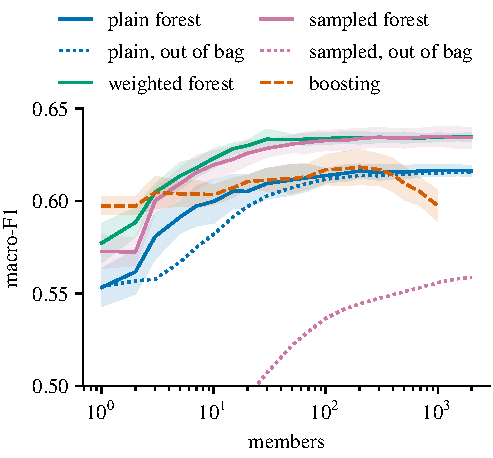
\includegraphics[width=\columnwidth]{../figures/ensemble/size.pdf}
\caption{Effect of the number of members}
\label{fig:size}
\end{figure}

Figure~\ref{fig:features} shows the effect of the number $\varphi$ of features tried per split. The score rose from \OFeatOneF{} at one feature to \OFeatEightF{} at the default square root, peaked at \OFeatSixteenF{} with 16 features and fell to \OFeatAllF{} for plain bagging. The strength of a tree rose only from \OFeatOneS{} to \OFeatAllS{}, whereas the disagreement fell from \OFeatOneA{} to \OFeatAllA{} and the Yule statistic $\mathcal{Q}$ rose from \OFeatOneQ{} to \OFeatAllQ{}, so the trees erred more often together. A trade-off between strength and diversity therefore existed, but the strength varied little. The diversity moved monotonically with $\varphi$ while the score peaked in the middle of the range, in line with the doubt that Kuncheva and Whitaker raised~\cite{kuncheva2003}. The default square root was not the optimum.

\begin{figure*}[t]
\centering
\begin{subfigure}[t]{0.32\textwidth}
\centering
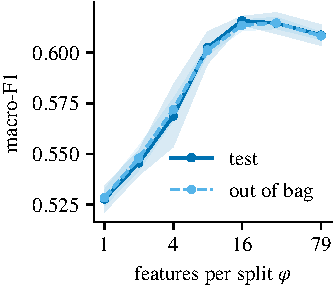
\includegraphics{../figures/ensemble/features_f1.pdf}
\caption{Score}
\end{subfigure}
\hfill
\begin{subfigure}[t]{0.32\textwidth}
\centering
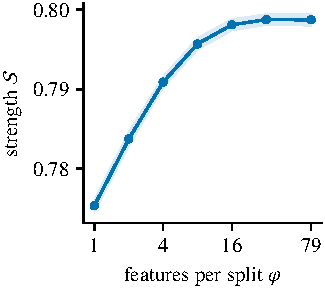
\includegraphics{../figures/ensemble/features_strength.pdf}
\caption{Strength $\mathcal{S}$}
\end{subfigure}
\hfill
\begin{subfigure}[t]{0.32\textwidth}
\centering
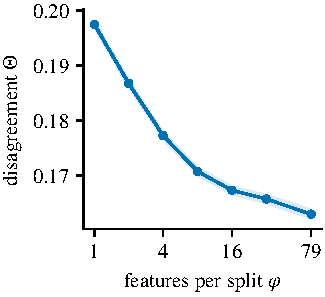
\includegraphics{../figures/ensemble/features_disagreement.pdf}
\caption{Disagreement $\Theta$}
\end{subfigure}
\caption{Effect of the number of features per split $\varphi$ on the forest}
\label{fig:features}
\end{figure*}

Deep trees with small leaves gave the highest score, as expected for averaging. The score grew from \ODepthThreeLeafOneF{} at depth three to \ODepthNoneLeafOneF{} without a depth limit, and fell to \ODepthNoneLeafFiftyF{} at a leaf size of 50 while the accuracy changed little. The loss lay in the rare classes: the recall of Worms fell from \OLeafOneRSeven{} at a leaf size of one to \OLeafTwentyFiveRSeven{} at 25. A large leaf stops the trees from splitting off the small pockets of a rare class, even though the strength of a single tree rose with the leaf size.

\subsection{Class Treatment and Tuned Ensembles}
\label{sec:res-treatment}

A mild balanced bootstrap gave the largest gain at a small cost in accuracy, as Table~\ref{tab:treatment} shows. The balanced bootstrap with the exponent 0.5 raised the macro-averaged F1 score by \OTrEffBootHalf{}, with a paired effect size of \OTrEffSizeBootHalf{}, and the recall of Worms from \OTrPlainRSeven{} to \OTrBootHalfRSeven{}. Class weights with the power 0.5 gained \OTrEffWeightHalf{}. Stronger treatments lowered the score again, because the precision of the rare classes fell faster than the recall rose. Undersampling to the smallest class gave the highest balanced accuracy but the lowest score. Combining class weights with the balanced bootstrap gave \OTrBootHalfWeightHalfF{}, below either treatment alone, so the two treatments overlap. The recall of Worms varied by \OTrPlainRSevenStd{} between units for the plain forest, so only large differences on the class are reliable.

% Generated by code/ensemble/make_report_numbers.py. Do not edit by hand.
\begin{table}[t]
\caption{Class treatment of the forest}
\label{tab:treatment}
\centering
\footnotesize
\setlength{\tabcolsep}{1.5pt}
\begin{tabular}{llcccccc}
\toprule
 & & & & & \multicolumn{3}{c}{Recall $e_j$} \\
\cmidrule(l){6-8}
Sampler & $\alpha$ & Macro-F1 & Acc. & Bal. acc. & Backdoor & Analysis & Worms \\
\midrule
standard & 0 & 0.601 $\pm$ .009 & 0.832 & 0.574 & 0.092 & 0.112 & 0.446 \\
standard & 0.5 & 0.614 $\pm$ .007 & 0.825 & 0.603 & 0.124 & 0.123 & 0.546 \\
standard & 1 & 0.592 $\pm$ .008 & 0.800 & 0.588 & 0.189 & 0.152 & 0.575 \\
$\omega = 0.5$ & 0 & 0.631 $\pm$ .003 & 0.823 & 0.640 & 0.168 & 0.140 & 0.690 \\
$\omega = 1$ & 0 & 0.588 $\pm$ .005 & 0.774 & 0.617 & 0.223 & 0.166 & 0.712 \\
under 1,000 & 0 & 0.531 $\pm$ .006 & 0.728 & 0.650 & 0.229 & 0.276 & 0.889 \\
under Worms & 0 & 0.481 $\pm$ .003 & 0.709 & 0.661 & 0.326 & 0.309 & 0.946 \\
\bottomrule
\end{tabular}
\end{table}


The joint search confirmed the sweeps. In the second stage, the three families with a class treatment were equivalent: the weighted forest reached \OJWeightedF{} $\pm$ \OJWeightedFStd{}, the sampled forest \OJSampledF{} $\pm$ \OJSampledFStd{} and the forest with both treatments \OJBothF{} $\pm$ \OJBothFStd{}. The data therefore do not separate the class weights from the balanced bootstrap. The plain forest scored lower by \OJPlainGap{}. The weighted forest uses \OJWeightedFeatures{} features per split, depth \OJWeightedDepth{}, a leaf size of \OJWeightedLeaf{} and $\alpha = \OJWeightedAlpha$. The sampled forest uses \OJSampledFeatures{} features, fully grown trees and $\omega = \OJSampledOmega$, and the plain forest \OJPlainFeatures{} features.

Boosting needed deep weak learners. The best grid score rose from \OBoostGridDepthThreeBest{} at depth three to \OBoostGridDepthTwentyFourBest{} at depth 24 and fell to \OBoostGridDepthThirtyTwoBest{} at depth 32. The tuned ensemble uses depth \OBoostTunedDepth{}, the learning rate \OBoostTunedRate{}, the class-weight power \OBoostTunedAlpha{} and \OBoostTunedRounds{} rounds, and scored \OBoostTunedF{} $\pm$ \OBoostTunedFStd{}. Even deep learners stayed below the weighted forest.

\subsection{Bias, Variance and Boosting Weight}
\label{sec:res-bias}

Table~\ref{tab:decomposition} gives the decomposition over the \OBvFolds{} tuning folds, with \OBvSets{} training sets of \OBvRows{} instances per fold. Differences above 0.01 are stable over the folds.

% Generated by code/ensemble/make_report_numbers.py. Do not edit by hand.
\begin{table}[t]
\caption{Bias and variance}
\label{tab:decomposition}
\centering
\footnotesize
\setlength{\tabcolsep}{3pt}
\begin{tabular}{lcccccc}
\toprule
Model & $\mathcal{E}$ & $\beta$ & $\beta_{\mathrm{o}}$ & $\mathcal{N}$ & $\mathcal{V}$ & Macro-F1 \\
\midrule
tree & 0.200 & 0.176 & 0.117 & +0.024 & 0.111 & 0.554 $\pm$ 0.001 \\
tree, balanced & 0.259 & 0.249 & 0.250 & +0.010 & 0.114 & 0.551 $\pm$ 0.004 \\
bagging & 0.178 & 0.173 & 0.112 & +0.005 & 0.068 & 0.588 $\pm$ 0.004 \\
forest, plain & 0.175 & 0.171 & 0.110 & +0.004 & 0.065 & 0.593 $\pm$ 0.005 \\
forest, weighted & 0.184 & 0.180 & 0.154 & +0.004 & 0.059 & 0.611 $\pm$ 0.005 \\
forest, sampled & 0.192 & 0.184 & 0.152 & +0.008 & 0.084 & 0.598 $\pm$ 0.004 \\
boosting & 0.196 & 0.182 & 0.151 & +0.014 & 0.095 & 0.578 $\pm$ 0.005 \\
\bottomrule
\end{tabular}
\end{table}


The plain forest lowered the error of the tree by \OBvRfErrorDrop{}: the net variance $\mathcal{N}$ fell by \OBvRfNetDrop{} and the bias by \OBvRfBiasDrop{}. Within the operational definitions of Section~\ref{sec:procedure-measures}, about four fifths of the gain came from the reduction of the net variance, as expected. The variance $\mathcal{V}$ fell further, from \OBvTreeV{} to \OBvRfV{}, because $\mathcal{V}$ also counts the helpful differences. Plain bagging reached nearly the same error, so the random feature subsets added little at the training-set size of the decomposition. The class treatment moved errors from the rare classes to the frequent classes. The weighted forest kept the net variance of the plain forest, while the bias on Worms fell from \OBvRfBSeven{} to \OBvRfWBSeven{} and on denial of service (DoS) from \OBvRfBThree{} to \OBvRfWBThree{}. Per class, the decomposition locates the remaining error. On Backdoor and Analysis, the bias stayed at \OBvRfBTwo{} and \OBvRfBFive{} for the plain forest, against \OBvTreeBTwo{} and \OBvTreeBFive{} for the tree, with net variances of \OBvRfNTwo{} and \OBvRfNFive{}, so averaging had no variance left to remove on those classes. On Worms, the plain forest lowered the net variance from \OBvTreeNSeven{} to \OBvRfNSeven{} at a nearly unchanged bias. Even the weighted forest kept a bias of \OBvRfWBTwo{} on Backdoor and \OBvRfWBFive{} on Analysis. The sampled forest had a higher variance, because a balanced bootstrap repeats the few rare instances many times. Boosting shares the class weights of the weighted forest, so the weighted forest is the reference for boosting. Contrary to both expectations, boosting reduced the bias no further than the weighted forest and kept more variance than the forests, although less than the tree. The decomposition covered only the tuned deep learners.

Boosting placed nearly all of the instance weight on the conflicting vectors within the first rounds. Rows of conflicting vectors make up \OBwConfRows{} of the training rows, yet their share of the weight rose from \OBwConfOne{} after the first round to \OBwConfTen{} after ten rounds and \OBwConfHundred{} after 100 rounds. The conflicting vectors hold every row that no deterministic classifier can fit. The concentration and the decline after the peak agree with the conflicting rows driving the decline, but deep learners and class weights also shape the rounds.

\subsection{Out-of-Bag Error as a Validation Signal}
\label{sec:res-oob}

The out-of-bag score ranked distant configurations well and close configurations poorly. Figure~\ref{fig:oob} plots the out-of-bag against the test score of \OOobN{} forest configurations. The rank correlation was \OOobSpearmanF{} over all configurations and \OOobSpearmanHalfF{} above a test score of 0.5, but fell to \OOobSpearmanStageTwo{} within the close configurations of the second search stage. The out-of-bag accuracy differed from the test accuracy by \OOobDiffAcc{} on average.

\begin{figure}[t]
\centering
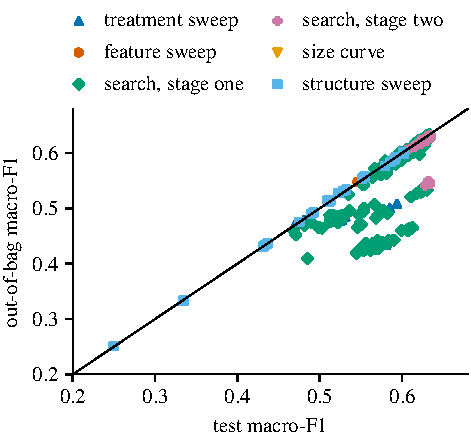
\includegraphics{../figures/ensemble/oob.pdf}
\caption{Out-of-bag against test score of all configurations}
\label{fig:oob}
\end{figure}

The out-of-bag macro-averaged F1 score lay below the test score by \OOobDiffFAbs{} on average, most of all for the class-balanced samplers in the cluster below the diagonal. A balanced bootstrap draws each instance of a rare class many times, so the instance is out of bag for few trees. Within the four families, the out-of-bag choice matched the cross-validated choice in \OOobFamSame{} families, with a largest loss of \OOobFamMaxRegret{}.

\subsection{Comparison under the Compatible Protocol}
\label{sec:res-comparison}

Every ensemble scored higher than the tree under the compatible protocol, as Table~\ref{tab:comparison} shows. The weighted forest scored higher than the tree by \OSCompRfWVsTreeMacroFAbsDiff{} in all 15 partitions, with \OSCompRfWVsTreeMacroFCor{} for the adjusted corrected t-test and \OSCompRfWVsTreeMacroFWil{} for the adjusted Wilcoxon test, and raised the balanced accuracy by \OSCompRfWVsTreeBalAccAbsDiff{}. The plain forest scored higher than the tree by \OSCompRfVsTreeMacroFAbsDiff{} (\OSCompRfVsTreeMacroFCor{}) and higher than the weighted nearest-neighbour model by \OSCompRfVsKnnCwMacroFAbsDiff{}. The sampled forest and boosting also scored higher than the tree, by \OSCompRfSVsTreeMacroFAbsDiff{} (\OSCompRfSVsTreeMacroFCor{}) and \OSCompBoostVsTreeMacroFAbsDiff{} (\OSCompBoostVsTreeMacroFCor{}), so all four gains over the tree were significant after the Holm adjustment. The gains were also practically large, between \OSCompBoostVsTreeMacroFMargins{} and \OSCompRfWVsTreeMacroFMargins{} times the equivalence margin. The two class-sensitive forests did not differ (\OSCompRfWVsRfSMacroFCor{}), whereas boosting scored lower than the weighted forest by \OSCompRfWVsBoostMacroFAbsDiff{} (\OSCompRfWVsBoostMacroFCor{}). Boosting and the plain forest differed by only \OSCompRfVsBoostMacroFAbsDiff{} (\OSCompRfVsBoostMacroFCor{}), a difference that is neither significant nor practically relevant. The gap to the weighted forest lies in the rare classes, as the accuracies differed by only \OSCompRfWVsBoostAccuracyPerK{} flows per thousand. The class treatment cost the plain forest \OSCompRfVsRfWAccuracyPerK{} correctly classified flows per thousand. On $G$, the paired bootstrap interval of the weighted forest against the tree, $[\OGDCompRfWVsTreeMacroFLo, \OGDCompRfWVsTreeMacroFHi]$, excludes zero. The intervals of the sampled against the weighted forest and of boosting against the plain forest include zero.

The gain came from the test instances without a training twin. On average, \OPCompShareNone{} per cent of the test instances had no twin, \OPCompShareCons{} per cent had twins of one label and \OPCompShareConf{} per cent had twins with conflicting labels. Every model classified the consistent twins almost perfectly and the conflicting twins poorly, the tree with accuracies of \OPCompTreeAccCons{} and \OPCompTreeAccConf{}. Without a twin, the accuracy rose from \OPCompTreeAccNone{} for the tree to \OPCompRfAccNone{} for the plain forest, the expected answer to the comparison question.

The class treatment raised the F1 score on $G$ of Worms from \OPcRfFSeven{} for the plain forest to \OPcRfWFSeven{} for the weighted forest, and of DoS from \OPcRfFThree{} to \OPcRfWFThree{}. Worms has only 35 instances in $G$, and every model stayed below 0.2 on Backdoor and Analysis. Figure~\ref{fig:confusion} shows the confusion of the weighted forest. More than half of the Backdoor and Analysis flows were predicted as DoS, and DoS and Exploits exchanged a quarter or more of the flows of each class. In $D$, \OConfTwo{} per cent of the Backdoor flows and \OConfFive{} per cent of the Analysis flows sit in vectors with conflicting labels, against \OConfZero{} per cent of the normal flows.

\begin{figure}[t]
\centering
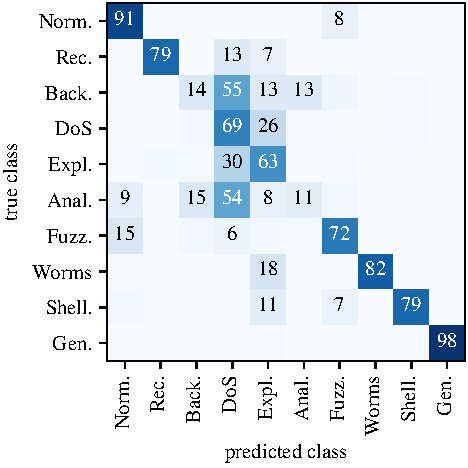
\includegraphics{../figures/ensemble/confusion.pdf}
\caption{Row-normalised confusion matrix of the weighted forest on $G$ in per cent}
\label{fig:confusion}
\end{figure}

A split of $G$ tests the role of the conflicting vectors. On the \OGcCleanRows{} per cent of the rows outside conflicting vectors, the weighted forest predicted \OGcCleanBackDoS{} per cent of the Backdoor flows and \OGcCleanAnalDoS{} per cent of the Analysis flows as DoS, against \OGcConfBackDoS{} and \OGcConfAnalDoS{} per cent inside conflicting vectors. The conflicting labels are therefore the main source of that confusion. The confusion of DoS with Exploits persisted on the clean rows, at \OGcCleanDoSExpl{} per cent, so the two classes overlap in the feature space beyond the identical vectors.

\subsection{Grouped Protocol and Dissimilar Ensembles}
\label{sec:res-grouped}

The grouped scores stayed close to the compatible scores, although no test vector had a twin. The plain nearest-neighbour model fell from \OPCompKnnMacroF{} to \OPGrpKnnMacroF{}, as expected for a memorising model. The accuracy was slightly higher on the grouped partitions, for a cause that is not established. The Kendall rank correlation of the mean scores of the eight models between the protocols was \OKendallAccuracy{} for the accuracy, \OKendallBalAcc{} for the balanced accuracy and \OKendallMacroF{} for the macro-averaged F1 score. Two pairs changed places: the two single trees, and the plain forest and boosting. Each of those pairs lay within the equivalence margin under one of the protocols. The weighted forest stayed above the weighted nearest-neighbour model by \OSGrpRfWVsKnnCwMacroFAbsDiff{} (\OSGrpRfWVsKnnCwMacroFCor{}), so the ranking of the ensembles above the single models held.

The gains over the tree did not shrink on the grouped partitions. The weighted forest scored higher than the tree by \OSGrpRfWVsTreeMacroFAbsDiff{} (\OSGrpRfWVsTreeMacroFCor{}), against \OSCompRfWVsTreeMacroFAbsDiff{} under the compatible protocol. The sampled forest gained \OSGrpRfSVsTreeMacroFAbsDiff{} against \OSCompRfSVsTreeMacroFAbsDiff{}, and boosting \OSGrpBoostVsTreeMacroFAbsDiff{} against \OSCompBoostVsTreeMacroFAbsDiff{}. Only the gain of the plain forest fell, from \OSCompRfVsTreeMacroFAbsDiff{} to \OSGrpRfVsTreeMacroFAbsDiff{}. All four gains stayed significant, each with \OSGrpRfVsTreeMacroFCor{}. The unchanged gains agree with Section~\ref{sec:res-comparison}, where the gain came from the test instances without a twin, the only kind of test instance in a grouped partition.

The single grouped split $G_{g}$ gave a different picture. On $G_{g}$, every model had a lower accuracy than on $G$, by \OGAccDropMinPerK{} to \OGAccDropMaxPerK{} flows per thousand. The gain over the tree was smaller for every ensemble. The gain of the weighted forest fell from $\OGDCompRfWVsTreeMacroF$ to $\OGDGrpRfWVsTreeMacroF$, that of the plain forest from $\OGDCompRfVsTreeMacroF$ to $\OGDGrpRfVsTreeMacroF$, that of the sampled forest from $\OGDCompRfSVsTreeMacroF$ to $\OGDGrpRfSVsTreeMacroF$ and that of boosting from $\OGDCompBoostVsTreeMacroF$ to $\OGDGrpBoostVsTreeMacroF$. The two generalisation sets hold different rows, and the 15 grouped partitions show no such shrinkage. The smaller gains on $G_{g}$ may therefore be specific to that one split, and the comparison is not an isolated causal estimate of the effect of the twins.

No dissimilar combination scored higher than the best forest. Under the compatible protocol, the vote of all four members scored \OPCompVoteAllMacroF{}, lower than the weighted forest by \OSCompVoteAllVsRfWMacroFAbsDiff{} (\OSCompVoteAllVsRfWMacroFCor{}), and the vote of the two forests scored \OPCompVoteForestsMacroF{}. The stacked ensemble scored \OPCompStackMacroF{}, within \OSCompStackVsRfWMacroFAbsDiff{} of the weighted forest, and lay below the weighted forest by \OSGrpStackVsRfWMacroFAbsDiff{} (\OSGrpStackVsRfWMacroFCor{}) under the grouped protocol. Leaving the tree out of the vote raised the score by \OSCompVoteNoTreeVsVoteAllMacroFAbsDiff{}, and leaving the nearest-neighbour model out lowered the score by \OSCompVoteNoKnnVsVoteAllMacroFAbsDiff{}. The nearest-neighbour model thus adds a little diversity, but the equal weights let the weaker members pull the vote below the strongest member. As expected, no combination improved on the best forest by more than 0.005.

\subsection{Discussion}
\label{sec:res-discussion}

Three findings cut across the questions. First, averaging saturates early and removes mainly variance. Much of the remaining bias sits in the attack categories whose flows share conflicting vectors, and neither more trees nor boosting reduced that part. Second, the rare classes respond to the class treatment and to deep trees with small leaves, not to the number of trees. A mild treatment raised the score by \OJPlainGap{} in the joint search. Third, the repeated vectors did not change the order of the models, and the evidence on the size of the gain is mixed. The gains held on the 15 grouped partitions, as the twin analysis predicts, but shrank on the single set $G_{g}$. The two generalisation sets differ in their rows, so the smaller gains on $G_{g}$ are consistent with an effect of the twins or with a property of that one split, not an inference of either.

The evidence on boosting has three levels. The observation is that boosting peaked and then declined, and that nearly all of the instance weight moved to the conflicting rows. The interpretation is that boosting fits label noise, in line with the finding of Breiman that forests are more robust to noise. However, establishing an unconfounded causal link requires a specific ablation design: pruning all minority labels within the conflicting vectors to produce a noise-free ground truth, training SAMME across boosting rounds on both the raw and pruned datasets, and measuring whether the late-round degradation slope flattens. Because this specific ablation was not run, label noise sensitivity remains the primary hypothesis consistent with the weight shift, rather than a proven cause.

Five limitations qualify the findings. First, the tuned configurations came from the development set that the comparison partitions reuse, although the baselines share the effect. Second, the 15 partitions overlap, so the tests remain optimistic after the correction, and the conclusions also rest on effect sizes and the generalisation sets. Third, Worms has about \nWormsFold{} test instances per fold and 35 in $G$, so the scores of Worms are noisy. Fourth, the study did not build gradient boosting. Fifth, published results on UNSW-NB15 use other partitions, class sets and preprocessing, so the study does not compare the present scores with the published scores.

\subsection{Summary}
\label{sec:res-summary}

The forests converged after 20 to 50 trees and gained mainly through a lower net variance, and a mild class treatment helped the rare classes. The ranking and the gains over the tree held on the grouped partitions, and only the grouped generalisation set showed smaller gains. Boosting scored lower than the weighted forest and placed nearly all of the instance weight on conflicting rows. No dissimilar ensemble scored higher than the best forest.

%%%%
\section{Conclusion}
\label{sec:conclusion}

The study measured how much ensembles of classification trees gain on imbalanced attack categories with conflicting vectors, and why. The Conclusion answers the research questions and states the limitations and future work.

\subsection{Answers to the Research Questions}
\label{sec:concl-findings}

The study built a random forest and the stagewise additive modelling using a multi-class exponential loss (SAMME) variant of adaptive boosting from scratch. Under the compatible protocol, the macro-averaged F1 score rose from \OPCompTreeMacroF{} for the tree to between \OPCompBoostMacroF{} and \OPCompRfWMacroF{} for the ensembles. All four gains over the tree were significant after the Holm adjustment under both protocols.

The returns of the forests diminished after 20 to 50 trees without overfitting, whereas boosting peaked at \OBoostPeakAt{} rounds and then degraded. As the number of features per split grew, the strength of a tree varied little while the diversity fell, and the optimum of 16 to 24 features lay above the default. Fully grown trees with small leaves were best. A mild class treatment raised the score, and class weights and the balanced bootstrap were equivalent on the partitions and on $G$. About four fifths of the gain of the plain forest came from a reduction of the net variance. The boosting weight moved to the rows of conflicting vectors, a shift that agrees with sensitivity to label noise but does not prove such sensitivity. The out-of-bag error estimated the accuracy closely but separated close configurations poorly. The ensembles scored higher than both models of the second assignment, and the gain came from the test instances without a twin. Under the grouped protocol, the ranking held and the gains over the tree did not shrink on the partitions, apart from a small decrease for the plain forest. The gains were smaller only on the single set $G_{g}$, whose rows differ from those of $G$. No dissimilar ensemble improved on the best forest.

\subsection{Limitations and Future Work}
\label{sec:concl-future}

The overlap of the partitions, the reuse of the development set and the small Worms class limit the precision of the conclusions. Boosting without the minority labels of the conflicting vectors would test the cause of the decline of boosting, and grouped and ungrouped splits of one pool of rows would isolate the effect of the twins. Gradient boosting and tuning under the grouped protocol are further directions.

\bibliography{refs_common,references}
\raggedbottom

\appendices
\section{Acronyms}
\label{app:acronyms}
The report uses the two acronyms listed below. UNSW-NB15, the name of the data set, and F1, the name of a score, are names rather than acronyms.

\smallskip
\noindent
\begin{tabular}{@{}lp{0.36\textwidth}@{}}
DoS & denial of service, an attack category \\
SAMME & stagewise additive modelling using a multi-class exponential loss \\
\end{tabular}

\section{Symbols}
\label{app:symbols}
The symbols follow in alphabetical order, Latin letters first and Greek letters second.

\newcommand{\sym}[2]{\par\noindent\hangindent=0.11\textwidth\hangafter=1\makebox[0.11\textwidth][l]{#1}#2}
\smallskip
\sym{$a_{i,j}$}{votes for class $j$ on instance $i$}
\sym{$B$, $c$}{number of members, member index}
\sym{$b_j$}{class weight of class $j$}
\sym{$D$, $G$}{development and generalisation set}
\sym{$D_{g}$, $G_{g}$}{grouped development and generalisation set}
\sym{$\mathcal{E}$}{error over training sets}
\sym{$e_j$}{recall of class $j$}
\sym{$f_j$, $\bar{f}$}{F1 score of class $j$, macro-averaged F1}
\sym{$g(t)$, $H(t)$}{Gini index and entropy}
\sym{$i$, $j$}{instance index, class index}
\sym{$h$, $h'$}{model indices}
\sym{$k$}{number of neighbours}
\sym{$m$}{number of classes}
\sym{$\mathcal{N}$}{net variance}
\sym{$N^{11}$, $N^{00}$}{instances where both or neither member is correct}
\sym{$N^{10}$, $N^{01}$}{instances where only one member is correct}
\sym{$n$, $n_j$}{training instances, of class $j$}
\sym{$P_{c,j}(\vect{x})$}{leaf proportion of class $j$}
\sym{$p_{c,i}$}{boosting weight of instance $i$}
\sym{$\mathcal{Q}$}{mean Yule statistic of member pairs}
\sym{$q$}{undersampling size per class}
\sym{$R$}{number of training sets}
\sym{$\mathcal{S}$}{strength of the members}
\sym{$s$}{candidate split}
\sym{$\mathcal{T}$}{evaluated set of instances}
\sym{$t$, $t_L$, $t_R$}{node and children}
\sym{$u_j$}{precision of class $j$}
\sym{$\mathcal{V}$}{variance}
\sym{$v$}{deviation of paired differences}
\sym{$w_i$}{vote weight of neighbour $i$}
\sym{$\vect{x}$, $\vect{x}_i$}{feature vector, of instance $i$}
\sym{$y_i$}{label of instance $i$}
\sym{$\hat{y}(\vect{x})$}{predicted class}
\sym{$\tilde{y}(\vect{x}_i)$}{out-of-bag prediction}
\sym{$z$}{number of partitions}
\sym{$\alpha$}{class-weight power}
\sym{$\beta$, $\beta_{\mathrm{o}}$}{bias against label, against best label}
\sym{$\gamma$}{paired effect size}
\sym{$\Delta(s,t)$}{impurity decrease}
\sym{$\eta_L$, $\eta_R$}{shares of the node weight}
\sym{$\Theta$}{disagreement of members}
\sym{$\iota$}{indicator function}
\sym{$\kappa$}{ratio of test to training size}
\sym{$\mu_c(\vect{x})$}{class predicted by member $c$}
\sym{$\nu_c$}{model weight of member $c$}
\sym{$\pi_{t,j}$}{class proportion at node $t$}
\sym{$\varrho$}{learning rate}
\sym{$\sigma_c$}{weighted error of member $c$}
\sym{$\tau$}{corrected t statistic}
\sym{$\phi$}{impurity measure}
\sym{$\varphi$}{features tried per split}
\sym{$\chi_{c,i}$}{multiplicity of instance $i$}
\sym{$\psi_i$, $\bar{\psi}$}{paired difference and mean}
\sym{$\xi_{i,h}$}{score of model $h$ on partition $i$}
\sym{$\omega$}{class-balance exponent}
\sym{$\Omega_k(\vect{x})$}{indices of the neighbours}
\par

\end{document}